\documentclass[10pt]{academydoc}
\pagestyle{plain}
\usepackage{graphicx}
\usepackage{subcaption}
\usepackage{seqsplit} 

% Set Document Details
\doctype{tb} % spec, proc, tb (Specification, Procedure, Technical Bulletin)
\docname{ACES Output Transform User Guide}
\altdocname{ACES Output Transform User Guide}

% Sets the document name used in header - usually an abbreviated document title
\docnumber{TB-2017-00x}
\committeename{Academy Color Encoding System (ACES) Project Committee}
\docdate{August 18, 2017}
\summary{ The Academy Color Encoding System (ACES) includes a variety of Output Transforms intended to support a wide range of display devices.  These devices include standard dynamic range digital cinema projectors, broadcast monitors, computer desktop displays, and high dynamic range displays.  Each of these devices may be configured differently and requires an ACES output transforms be used based on the specifics of the configuration.  This document is intended to be practical guide help end-users determine the proper ACES output transform to be used based on their devices, configurations, and workflows.
}


% Document Starts Here
\begin{document}

\maketitle

% This file contains the content for the Notices
\prelimsectionformat	% Change formatting to that of "Notices" section
\chapter[Notices]{\uppercase{Notices}}
%% Modify below this line %%

\copyright\the\year{} Academy of Motion Picture Arts and Sciences (A.M.P.A.S.). All rights reserved. This document is provided to individuals and organizations for their own internal use, and may be copied or reproduced in its entirety for such use. This document may not be published, distributed, publicly displayed, or transmitted, in whole or in part, without the express written permission of the Academy.

The accuracy, completeness, adequacy, availability or currency of this document is not warranted or guaranteed. Use of information in this document is at your own risk. The Academy expressly disclaims all warranties, including the warranties of merchantability, fitness for a particular purpose and non-infringement.

Copies of this document may be obtained by contacting the Academy at councilinfo@oscars.org.

``Oscars,'' ``Academy Awards,'' and the Oscar statuette are registered trademarks, and the Oscar statuette a copyrighted property, of the Academy of Motion Picture Arts and Sciences.

% This paragraph is optional.  Comment out if you wish to remove it.
This document is distributed to interested parties for review and comment. A.M.P.A.S. reserves the right to change this document without notice, and readers are advised to check with the Council for the latest version of this document.

% This paragraph is optional.  Comment out if you wish to remove it.
The technology described in this document may be the subject of intellectual property rights (including patent, copyright, trademark or similar such rights) of A.M.P.A.S. or others. A.M.P.A.S. declares that it will not enforce any applicable intellectual property rights owned or controlled by it (other than A.M.P.A.S. trademarks) against any person or entity using the intellectual property to comply with this document.

% This paragraph is optional.  Comment out if you wish to remove it.
Attention is drawn to the possibility that some elements of the technology described in this document, or certain applications of the technology may be the subject of intellectual property rights other than those identified above. A.M.P.A.S. shall not be held responsible for identifying any or all such rights. Recipients of this document are invited to submit notification to A.M.P.A.S. of any such intellectual property of which they are aware.

\vspace{10pt}
These notices must be retained in any copies of any part of this document. \newpage
% This file contains the content for the Revision History and 
\prelimsectionformat	% Change formatting to that of "Notices" section
\chapter{Revision History}
%% Modify below this line %%

\begin{tabularx}{\linewidth}{|l|l|X|}
    \hline
    Version & Date       & Description \\ \hline
    1.0     & xx/xx/2017 & Initial Version \\ \hline
    &   &   \\ \hline
    &   &   \\ \hline
    &   &   \\ \hline
\end{tabularx}

\vspace{0.25in} % <-- DO NOT REMOVE
\chapter{Related Academy Documents} % <-- DO NOT REMOVE
\begin{tabularx}{\linewidth}{|l|X|}
    \hline
    Document Name & Description \\ \hline
     & \\ \hline
     & \\ \hline
     & \\ \hline
     & \\ \hline
     & \\ \hline
\end{tabularx} \newpage

\tableofcontents \newpage

% This file contains the content for the Introduction
\unnumberedformat	    % Change formatting to that of "Introduction" section
\chapter{Introduction} 	% Do not modify section title
%% Modify below this line %%
ACES 1.0 includes thirteen Output Transforms that can be broadly characterized as applying to four different display types used in various configurations. (Table \ref{odt-display-types-table}) The display types include digital cinema projectors typically used in digital intermediate, motion picture mastering, and theatrical exhibition, standard dynamic range (SDR) broadcast displays used in editorial and on-set preview applications, high dynamic range (HDR) broadcast displays used in mastering an exhibition of HDR content, and computer desktop monitors such as those typically used in the creation of computer generated visual effects (VFX).

\begin{table}[ht!]
\centering
\begin{tabular}{cc}
\textbf{Output Transform (Short Name)}                              & \textbf{Display Type}                               \\ \hline
\multicolumn{1}{|l|}{ACES 1.0 Output - P3-DCI}                      & \multicolumn{1}{l|}{Digital Cinema Projector (SDR)} \\ \hline
\multicolumn{1}{|l|}{ACES 1.0 Output - P3-D60}                      & \multicolumn{1}{l|}{Digital Cinema Projector (SDR)} \\ \hline
\multicolumn{1}{|l|}{ACES 1.0 Output - DCDM}                        & \multicolumn{1}{l|}{Digital Cinema Projector (SDR)} \\ \hline
\multicolumn{1}{|l|}{ACES 1.0 Output - DCDM (P3 gamut clip)}        & \multicolumn{1}{l|}{Digital Cinema Projector (SDR)} \\ \hline
\multicolumn{1}{|l|}{ACES 1.0 Output - Rec.709}                     & \multicolumn{1}{l|}{SDR Broadcast Monitor}          \\ \hline
\multicolumn{1}{|l|}{ACES 1.0 Output - Rec.709 (D60 sim.)}          & \multicolumn{1}{l|}{SDR Broadcast Monitor}          \\ \hline
\multicolumn{1}{|l|}{ACES 1.0 Output - Rec.2020}                    & \multicolumn{1}{l|}{SDR Broadcast Monitor}          \\ \hline
\multicolumn{1}{|l|}{ACES 1.0 Output - P3-D60 ST2084 (1000 nits)}   & \multicolumn{1}{l|}{HDR Broadcast Monitor}          \\ \hline
\multicolumn{1}{|l|}{ACES 1.0 Output - P3-D60 ST2084 (2000 nits)}   & \multicolumn{1}{l|}{HDR Broadcast Monitor}          \\ \hline
\multicolumn{1}{|l|}{ACES 1.0 Output - P3-D60 ST2084 (4000 nits)}   & \multicolumn{1}{l|}{HDR Broadcast Monitor}          \\ \hline
\multicolumn{1}{|l|}{ACES 1.0 Output - Rec.2020 ST2084 (1000 nits)} & \multicolumn{1}{l|}{HDR Broadcast Monitor}          \\ \hline
\multicolumn{1}{|l|}{ACES 1.0 Output - sRGB}                        & \multicolumn{1}{l|}{Desktop Computer Display}       \\ \hline
\multicolumn{1}{|l|}{ACES 1.0 Output - sRGB (D60 sim.)}             & \multicolumn{1}{l|}{Desktop Computer Display}       \\ \hline
\end{tabular}
\caption[ACES 1.0 Output Device Transforms and Display Types]{ACES 1.0 Output Device Transforms and Display Types}
\label{odt-display-types-table}
\end{table}

The output device to be used with any particular device depends on the detailed configuration of that device.  This document is intended to be practical guide help end-users determine the proper ACES output transform to be used the configuration, workflow, and intended usage.  This document is intended to cover a series of common use cases.  There may be valid uses of the ACES output transforms that fall outside of the scope of this document. \newpage
% This section contains the content for the References
\numberedformat
\chapter{References}
The following standards, specifications, articles, presentations, and texts are referenced in this text:
%% Modify below this line %%

SMPTE ST 2065-1:2012, Academy Color Encoding Specification (ACES)

SMPTE ST 2084:2014, Dynamic Range Electro-Optical Transfer Function of Mastering Reference Displays

ITU-R Rec. BT.709, Parameter values for the HDTV standards for production and international programme exchange 

ITU-R Rec. BT.1886, Reference electro-optical transfer function for flat panel displays used in HDTV studio production

ITU-R Rec. BT.2020, Parameter values for ultra-high definition television systems for production and international programme exchange

ITU-R Rec. BT.2100, Image parameter values for high dynamic range television for use in production and international programme exchange

IEC 61966-2-1, Multimedia systems and equipment -- Colour measurement and management -- Part 2-1: Colour management -- Default RGB colour space -- sRGB \newpage

% This file contains the content for a main section
\numberedformat
%% Modify below this line %%

\clearpage
\chapter{Output Transform Applications}\label{ch:ot-app}


%%%% Application -- Theatrical Digital Intermediate (P3-DCI Calibrated Projector) %%%% 
\section{Theatrical Digital Intermediate (P3-DCI Calibrated Projector)}
\label{sec:ot-app-p3dci}

\subsection{Summary}
\label{subsec:summary-p3dci}

It is common in the digital intermediate process (DI) to color correct
motion pictures and episodic television shows while displaying the
images using a DCI compliant digital cinema projector. DCI compliant
digital cinema projectors have a simplified setup using a projector
configuration file (PCF) that contains all the relevant projector
settings and can often be loaded at the press of a button. The most
common PCF used in motion picture and television production is the
``DCI-P3'' PCF. Using this PCF, the projector will be configured such
that equal red, green, and blue projector code values will produce the
chromaticity x=0.3140 y=0.3510 on the screen. With the projector
configured in this manner it is recommended that the ACES 1.0 ODT with
the transformID \texttt{\seqsplit{ODT.Academy.P3DCI\_48nits.a1.0.3}} be used.

\subsection{Projector Setup}
\label{subsec:setup-p3dci}

\begin{table}[ht!]
    \centering
        \begin{tabular}{|p{1.25in}|p{3in}|}
            \hline
            \textbf{Parameter} & \textbf{Setting} \\ \hline
            PCF & DCI-P3 (RGB 4:4:4 Full Range, P3 Primaries, DCI white point, 48 nit max Luminance) \\ \hline
            Viewing Environment & Dark \\ \hline
            Bit Depth & 12-bit \\ \hline 
    \end{tabular}
    \caption[Theatrical DI (P3DCI) - Projector Setup]{\small P3-DCI Projector Setup} 
    \label{tab:setup-p3dci}
\end{table}

\subsection{Best ODT for application} 
\label{subsec:bestODT-p3dci}

\begin{table}[ht!]
    \centering
    \begin{tabular}{|p{1.5in}|p{3in}|}
        \hline
        \textbf{Simple Name} & \textbf{TransformID} \\ \hline
        ACES 1.0 Output - P3-DCI & \texttt{\seqsplit{ODT.Academy.P3DCI\_48nits.a1.0.3}} \\ \hline
    \end{tabular}
    \caption[Theatrical DI (P3DCI) - Best ODT ]{\small P3-DCI Best ODT} 
    \label{tab:bestODT-p3dci}
\end{table}

\subsection{Notes}
\label{subsec:notes-p3dci}

Using the ``DCI-P3'' PCF, the projector will be configured such that
equal red, green, and blue display code values will produce the
chromaticity x=0.3140 y=0.3510 on the screen. However, the
\texttt{\seqsplit{ODT.Academy.P3DCI\_48nits.a1.0.3}} transform is configured such
that neutral ACES source file values (ACES R=G=B) will produce non-equal
projector code values. The chromaticity of produced on screen by those
non-equal projector code values will be x=0.32168 y=0.33767 (aka D60).

It's important to note that the image on projection screen may look
distinctly less green then some workflows that utilize a projector setup
with the ``DCI-P3'' PCF. This will also be reflected on the color
corrector scopes when neutral ACES values sent through the
\texttt{\seqsplit{ODT.Academy.P3DCI\_48nits.a1.0.3}} transform. (Figure \ref{fig:acesSource-p3dci}, \ref{fig:hist-p3dci}, \ref{fig:parade-p3dci}, \ref{fig:wf-p3dci}, \ref{fig:vect-p3dci}) For instance,
neutral ACES values processed through
\texttt{\seqsplit{ODT.Academy.P3DCI\_48nits.a1.0.3}} will not have equal levels on
the waveform, nor will they land in the middle of the vector scope. This behavior was intentional. The image may also
have a distinctly magenta cast on a computer monitor such as the one
used for the color corrector user interface if that monitor is
calibrated to a D65 white point. (Figure \ref{fig:cv-p3dci}) Although not noted in the
name of this ODT, the mimics the behavior found in other ODTs included
in ACES 1.0 and labeled ``D60 sim''. Due to this ``D60 sim'' behavior
the maximum output screen luminance of neutral ACES values will be
slightly less than the maximum luminance produced by projector code
values red = 1, green = 1, blue = 1 (e.g.~48 nits).

When using the correct projector setup and corresponding ODT, the image
on the projector screen will match nearly exactly in Application \ref{sec:ot-app-p3dci} and
Application \ref{sec:ot-app-p3d60}.

    \begin{figure*}[ht!]
        \centering
        \begin{subfigure}[b]{0.475\textwidth}
            \centering
            
\includegraphics[width=\textwidth]{images/aces}
            \caption[Source ACES Image]%
            {{\small ACES Image}}    
            \label{fig:acesSource-p3dci}
        \end{subfigure}
        \hfill
        \begin{subfigure}[b]{0.475\textwidth}  
            \centering 
            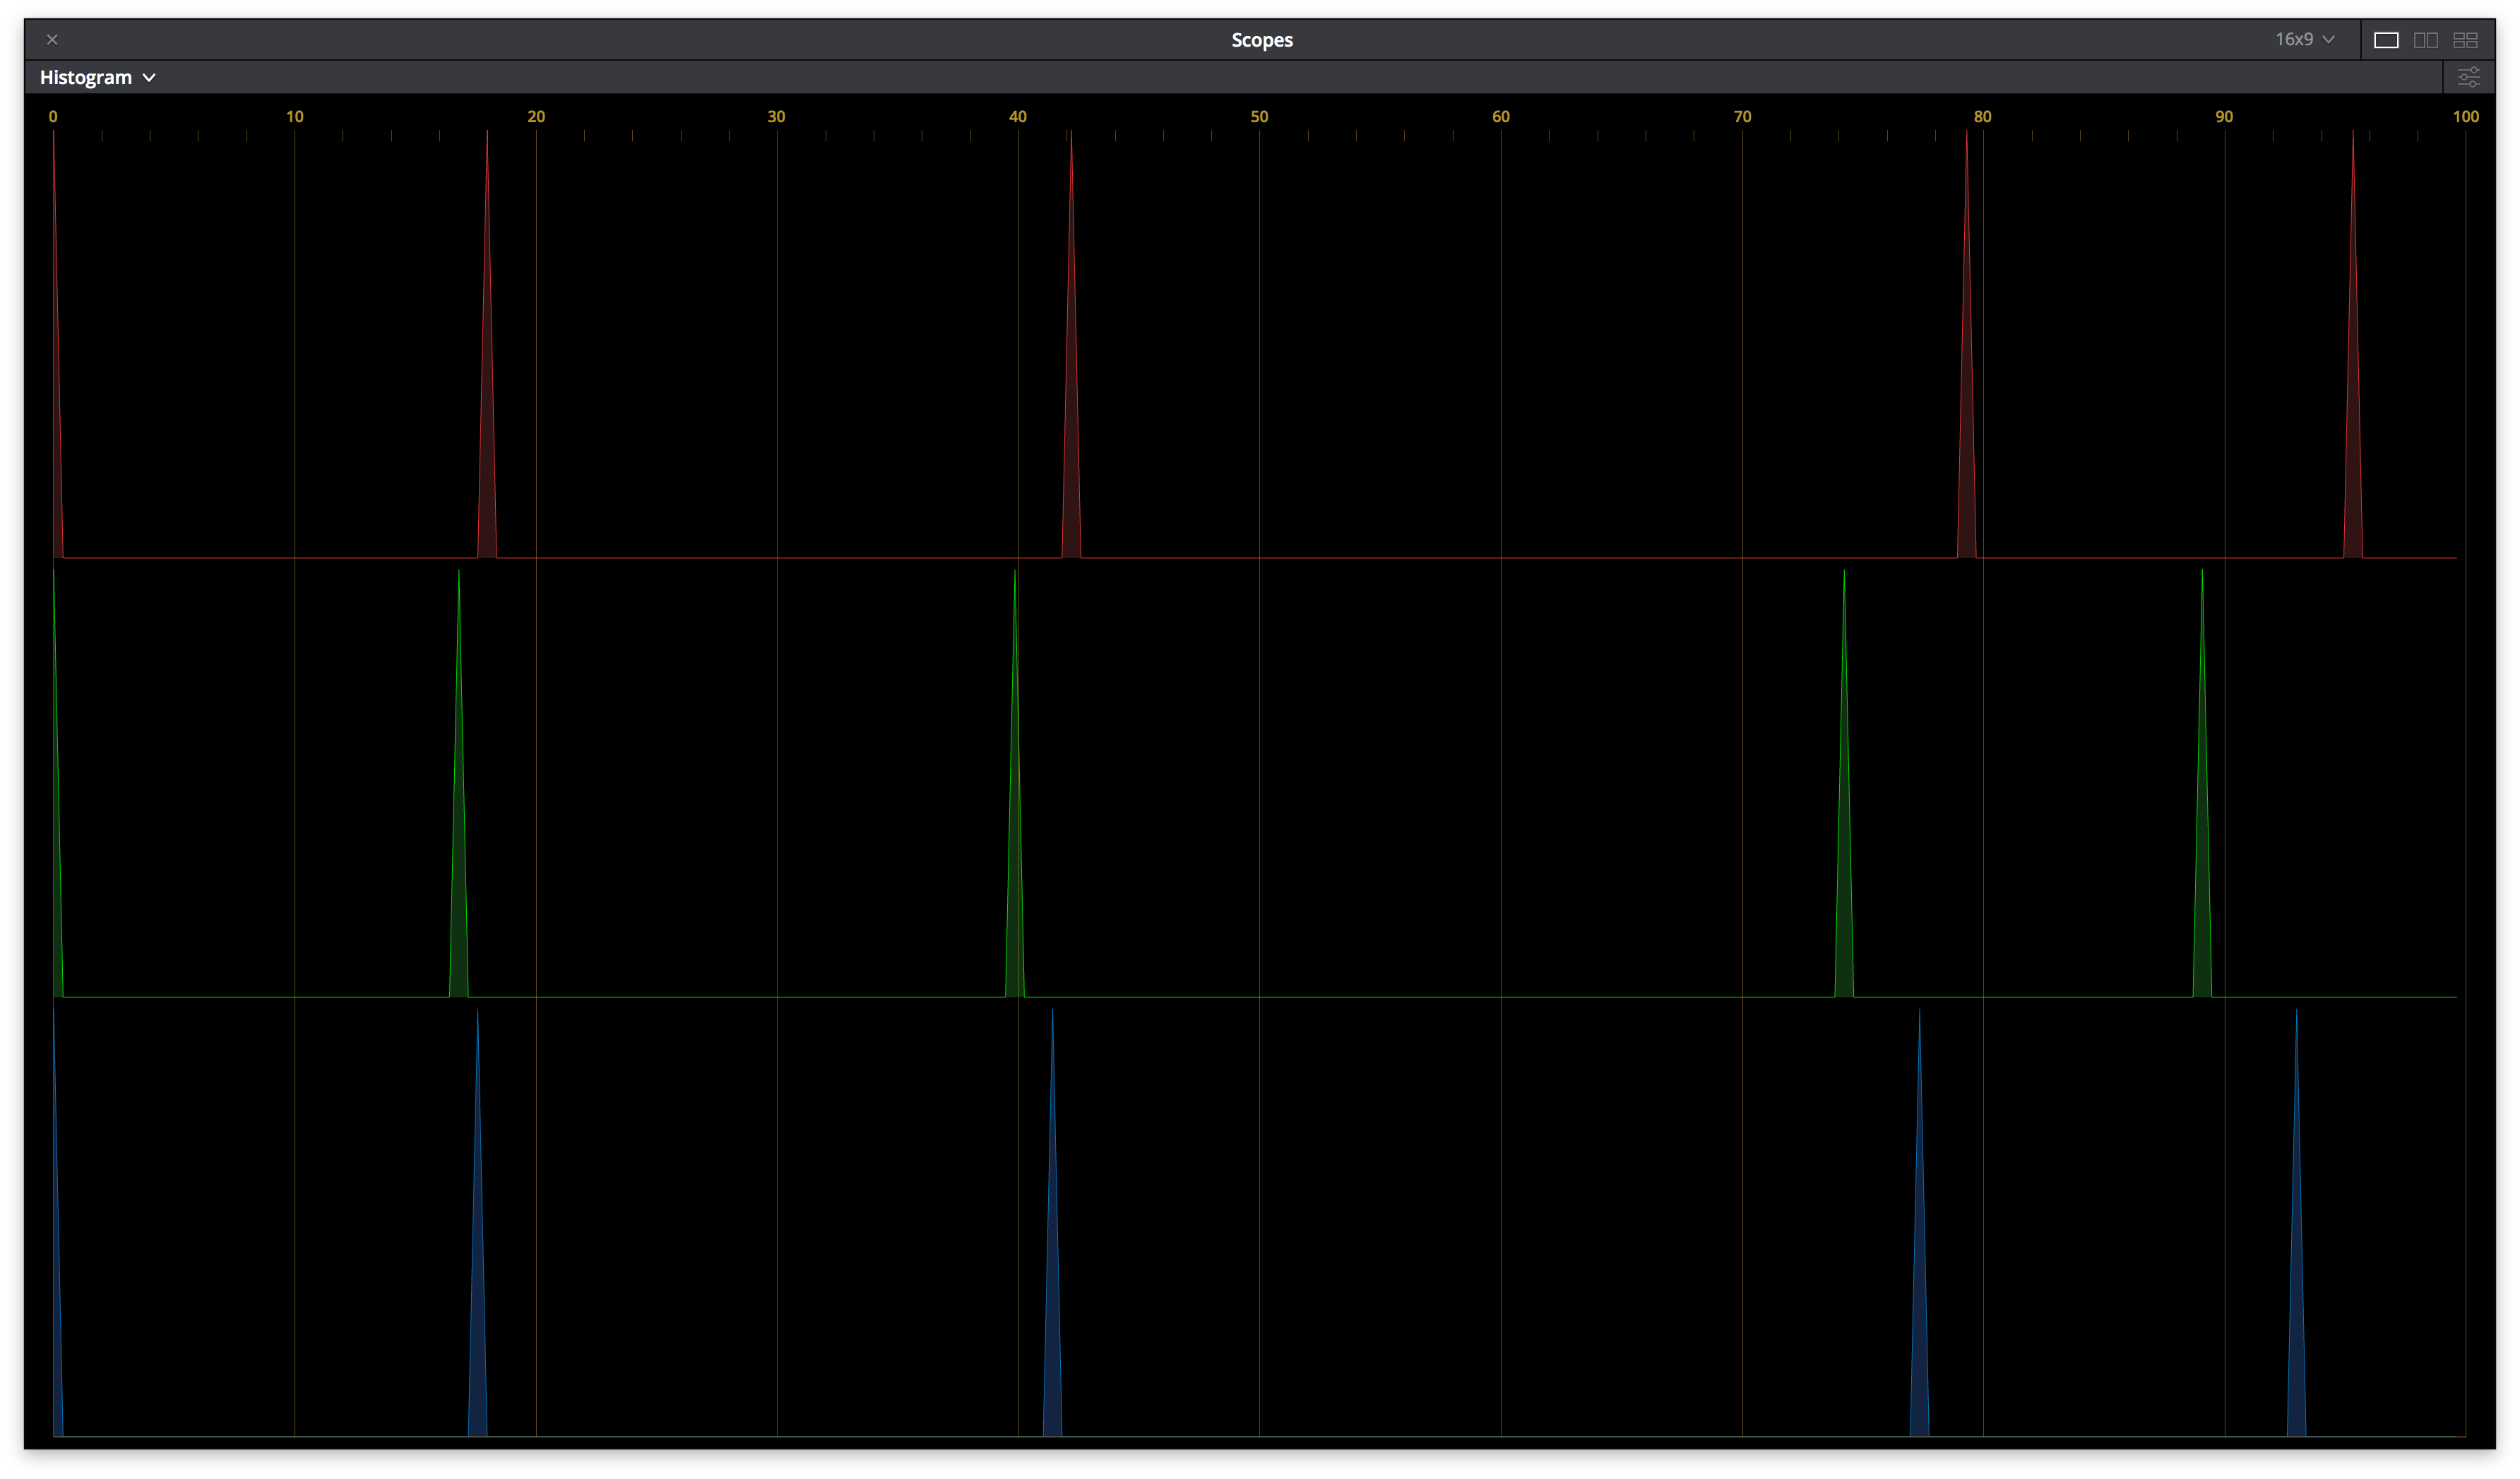
\includegraphics[width=\textwidth]{images/p3dci/p3dci_histogram}
            \caption[Histogram]%
            {{\small Histogram}}    
            \label{fig:hist-p3dci}
        \end{subfigure}
        \vskip\baselineskip
        \begin{subfigure}[b]{0.475\textwidth}   
            \centering 
            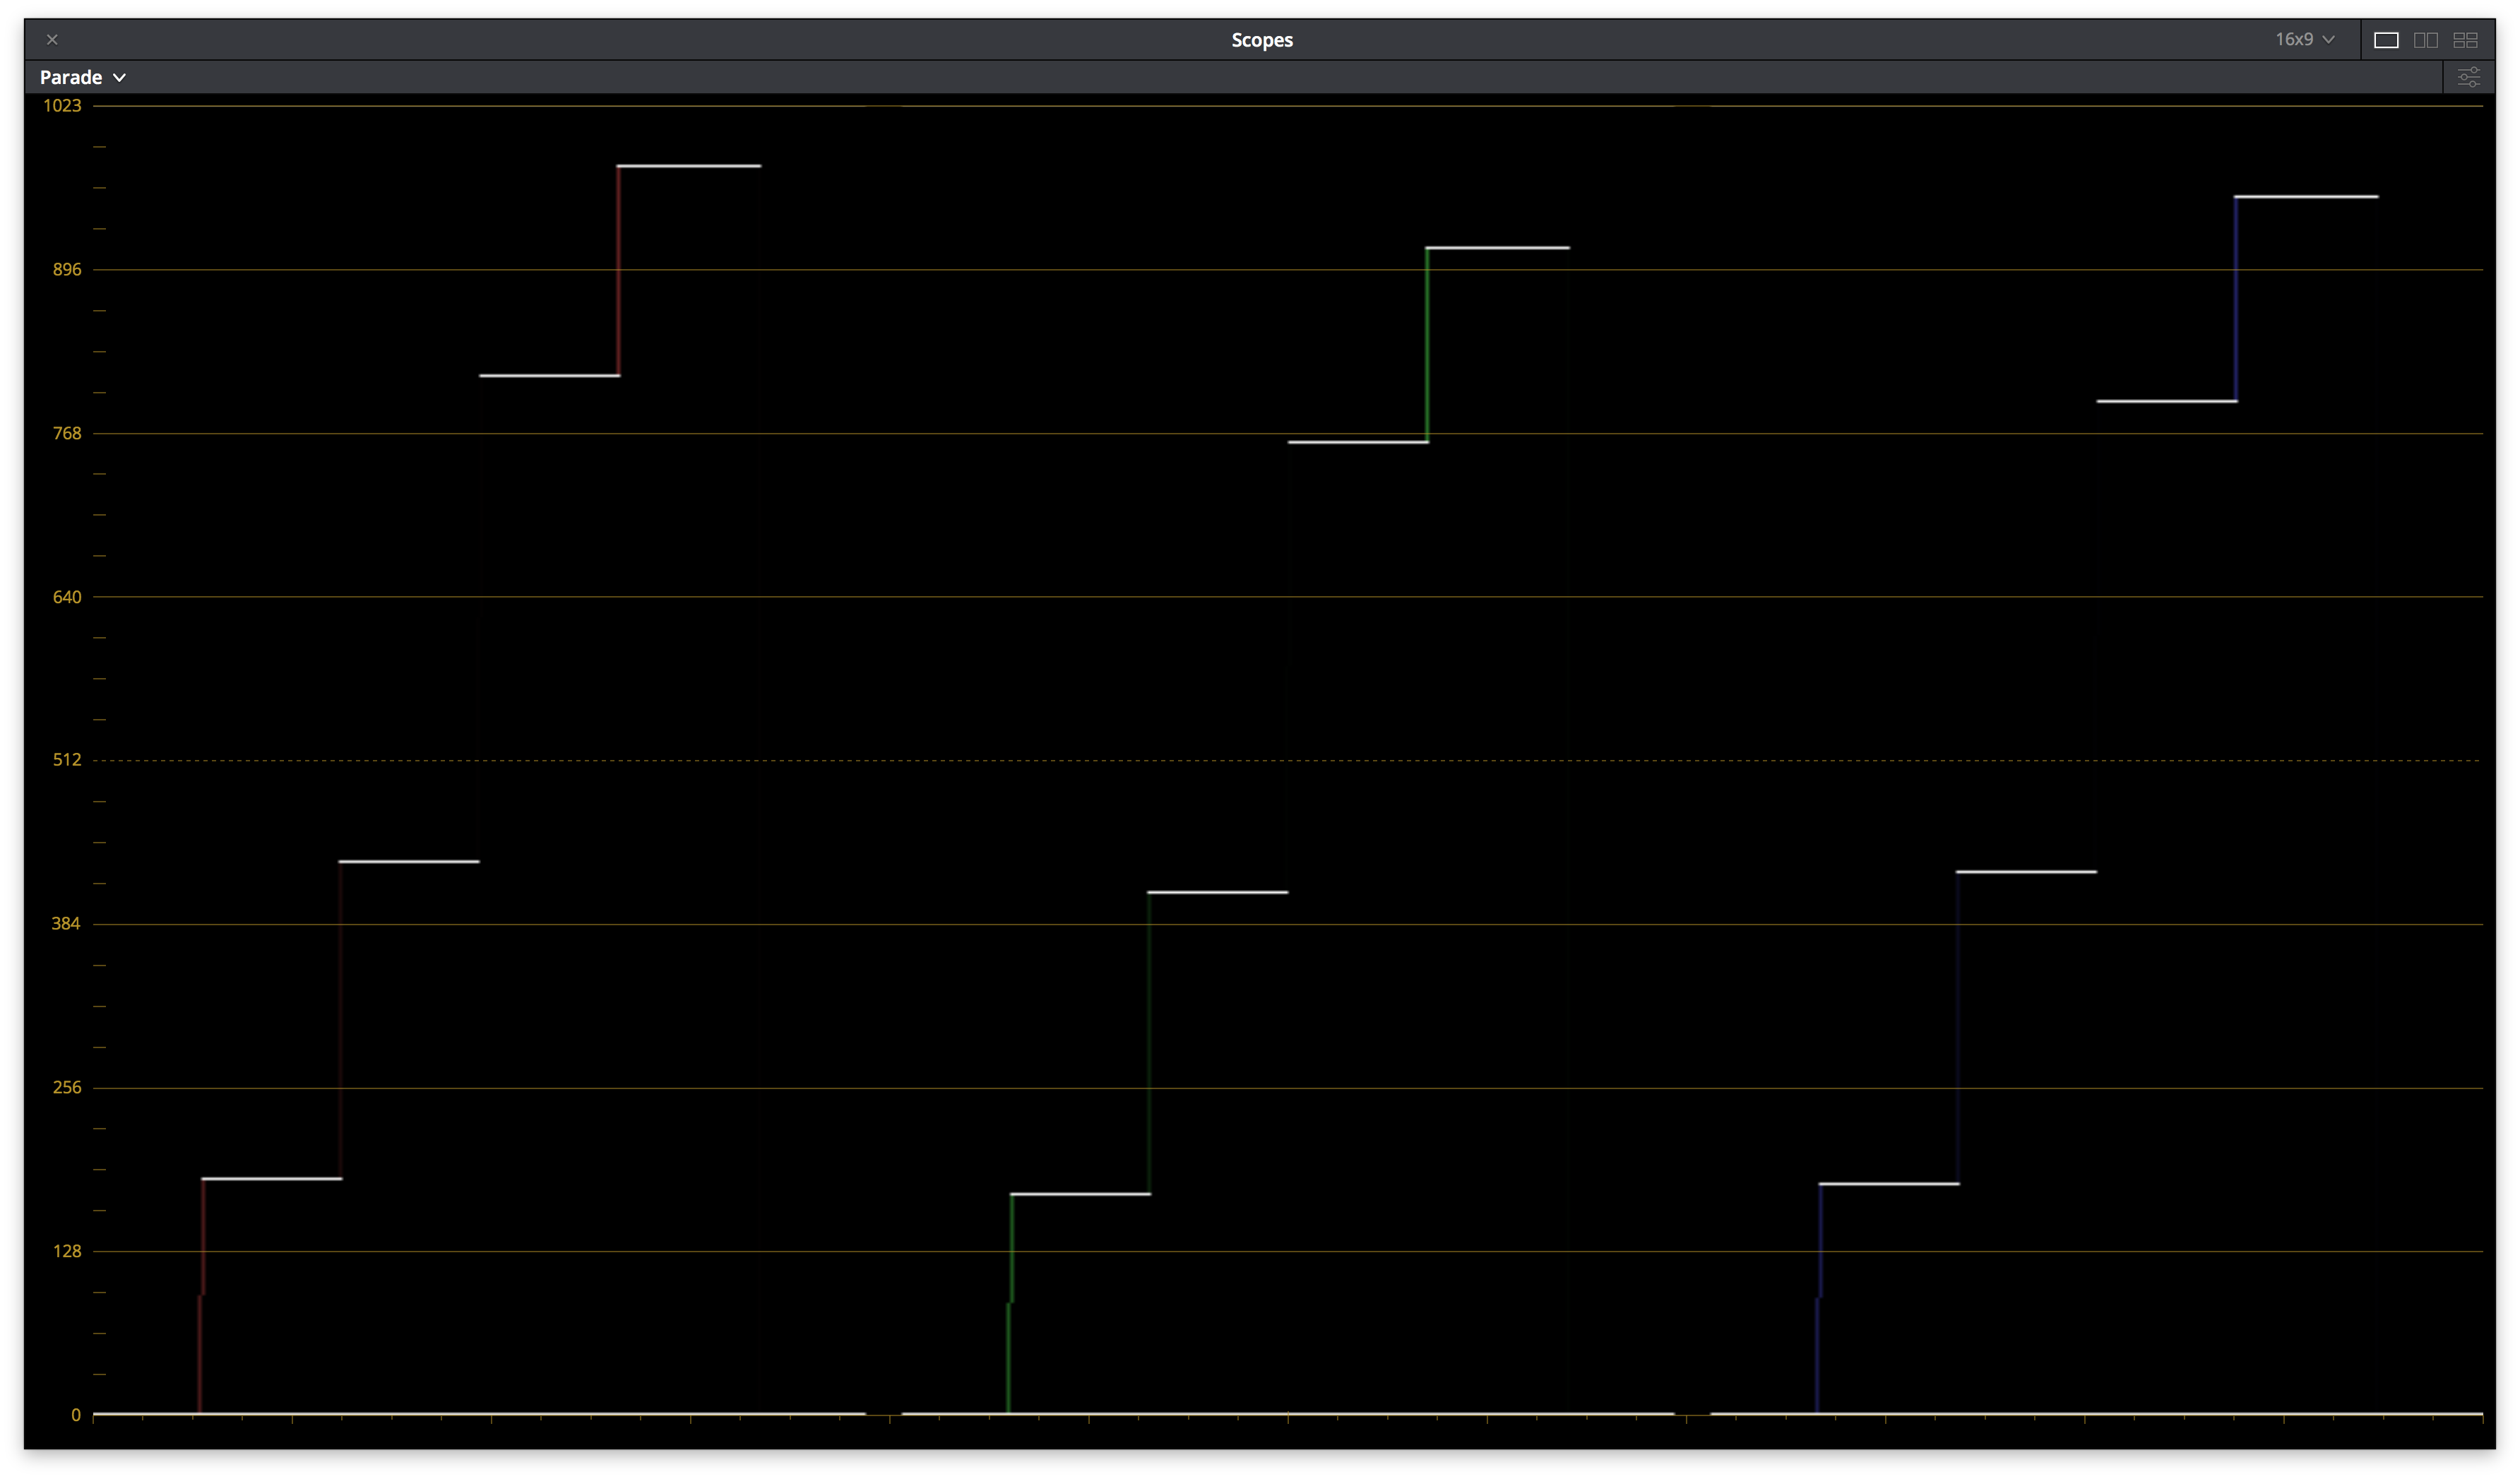
\includegraphics[width=\textwidth]{images/p3dci/p3dci_parade}
            \caption[Parade]%
            {{\small Parade}}    
            \label{fig:parade-p3dci}
        \end{subfigure}
        \quad
        \begin{subfigure}[b]{0.475\textwidth}   
            \centering 
            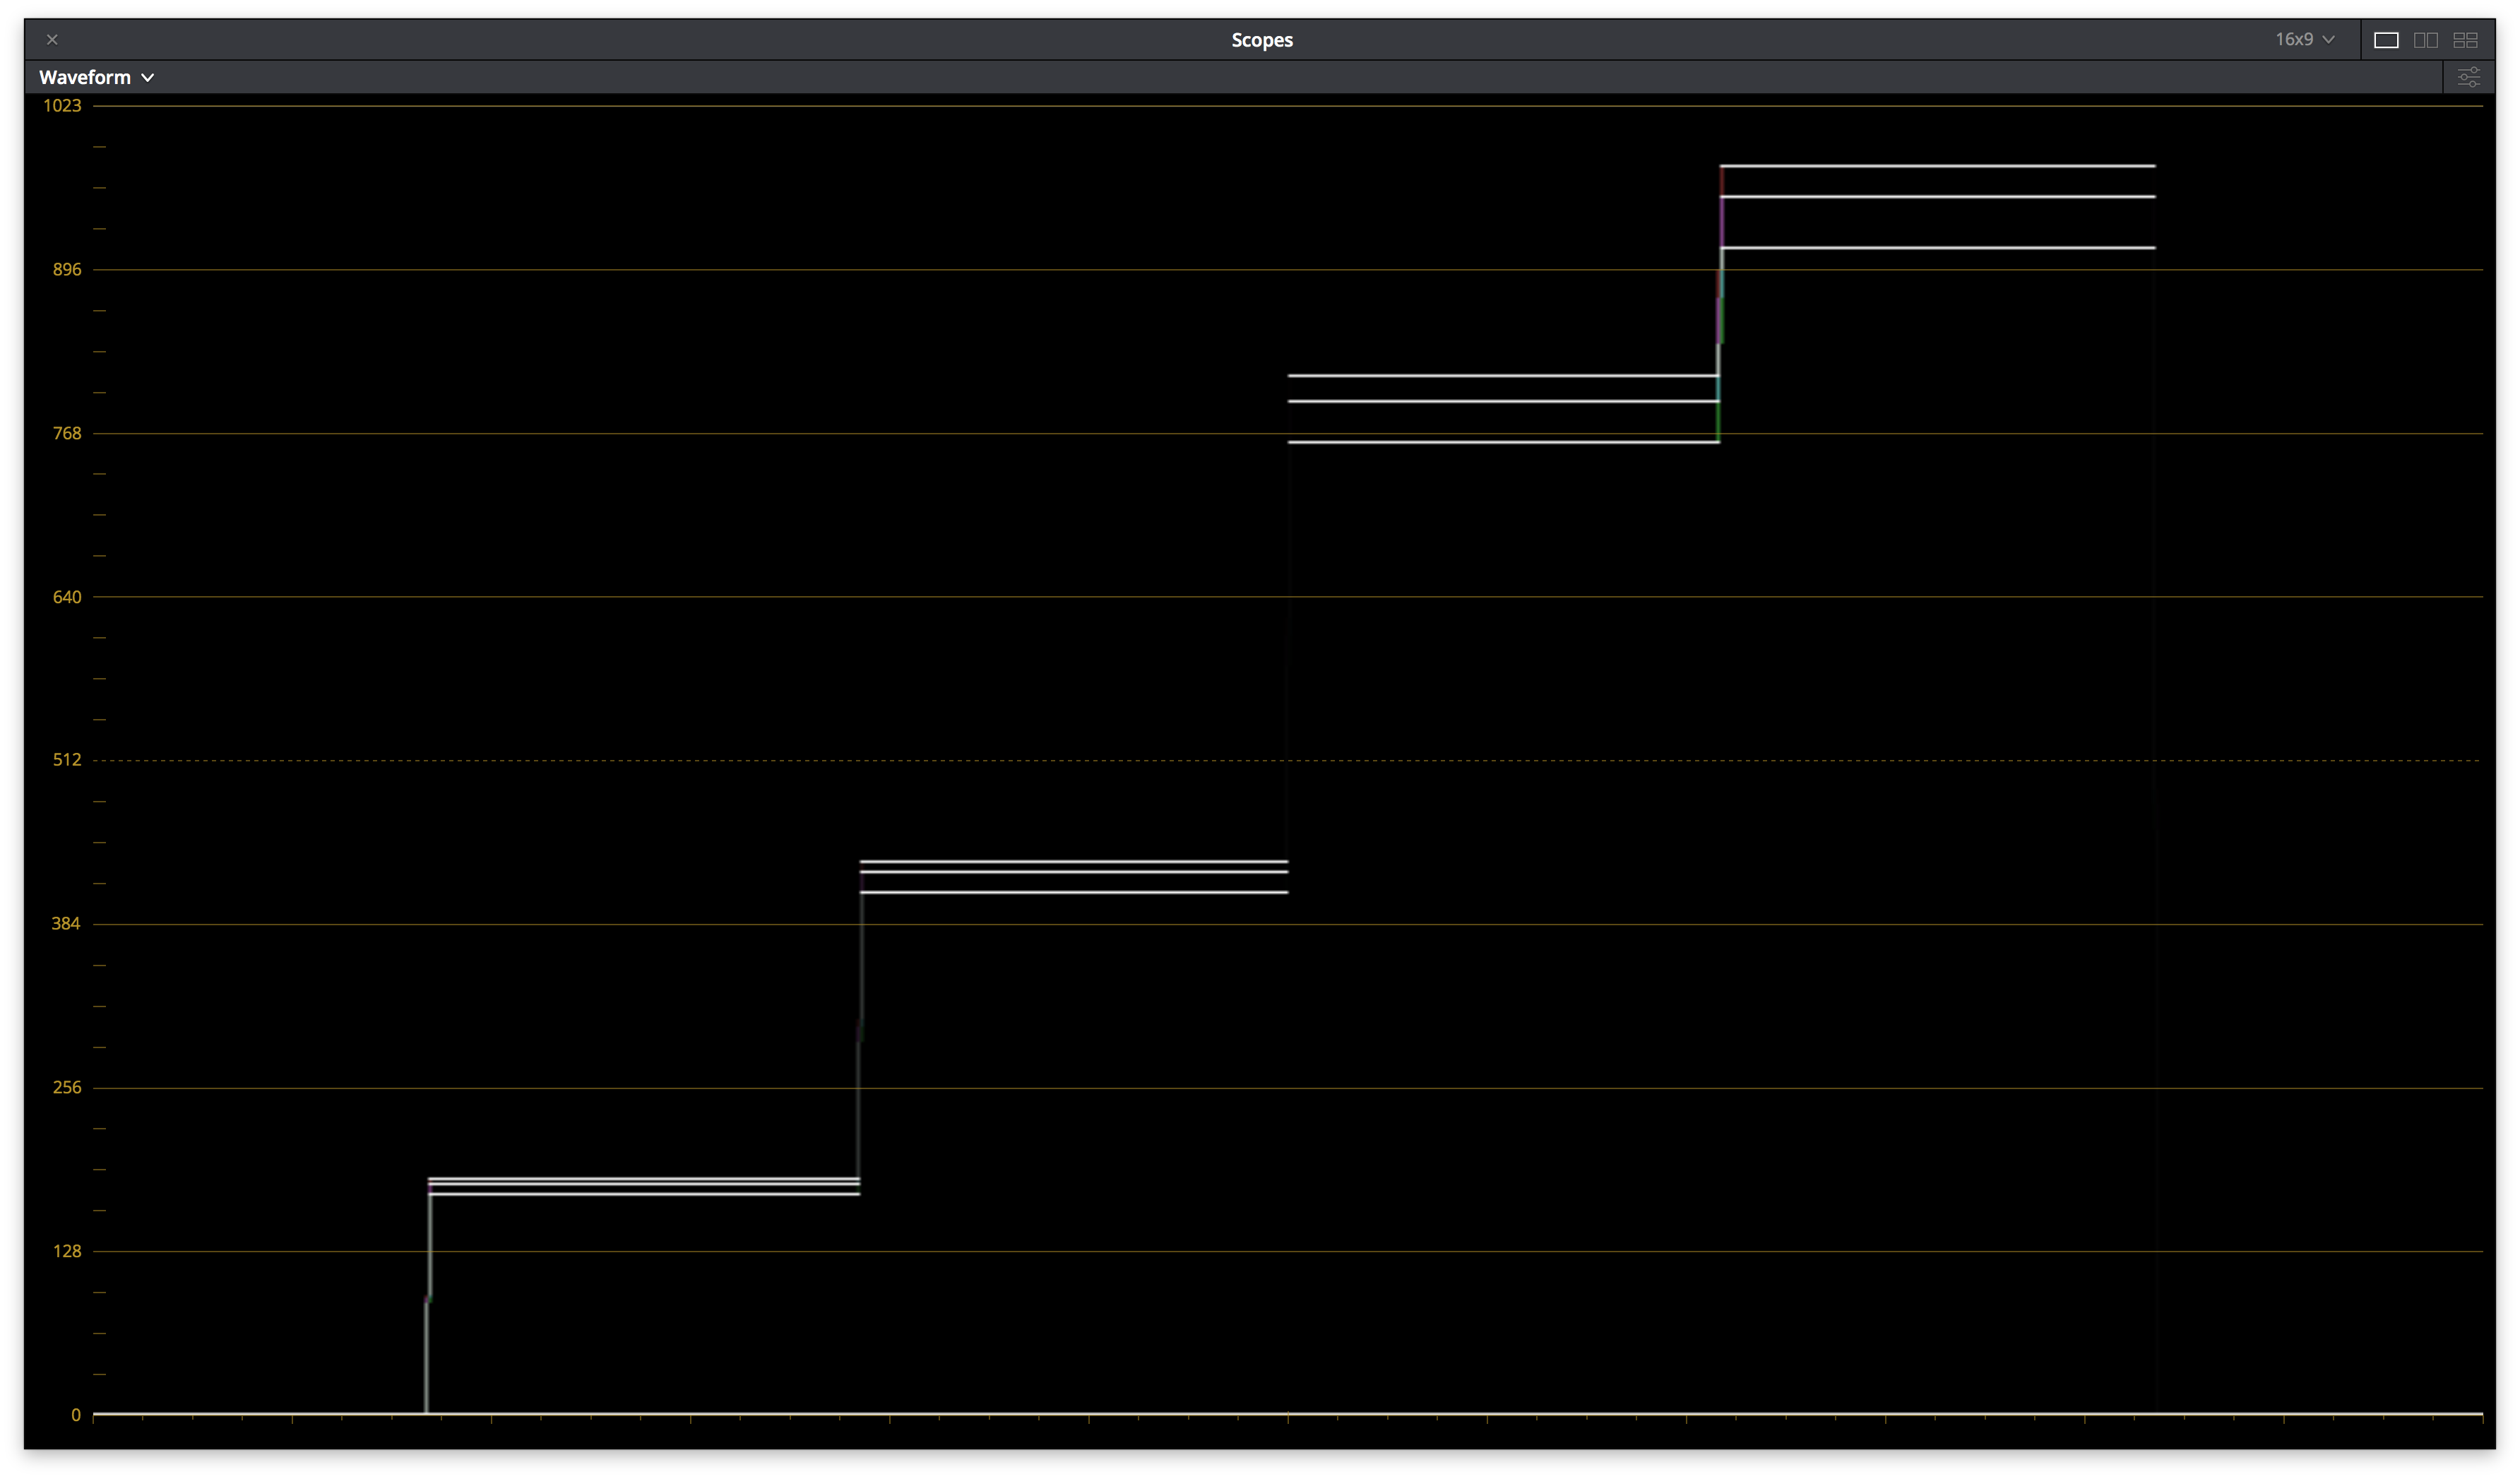
\includegraphics[width=\textwidth]{images/p3dci/p3dci_waveform}
            \caption[]%
            {{\small Waveform}}    
            \label{fig:wf-p3dci}
        \end{subfigure}
        \begin{subfigure}[b]{0.475\textwidth}   
            \centering 
            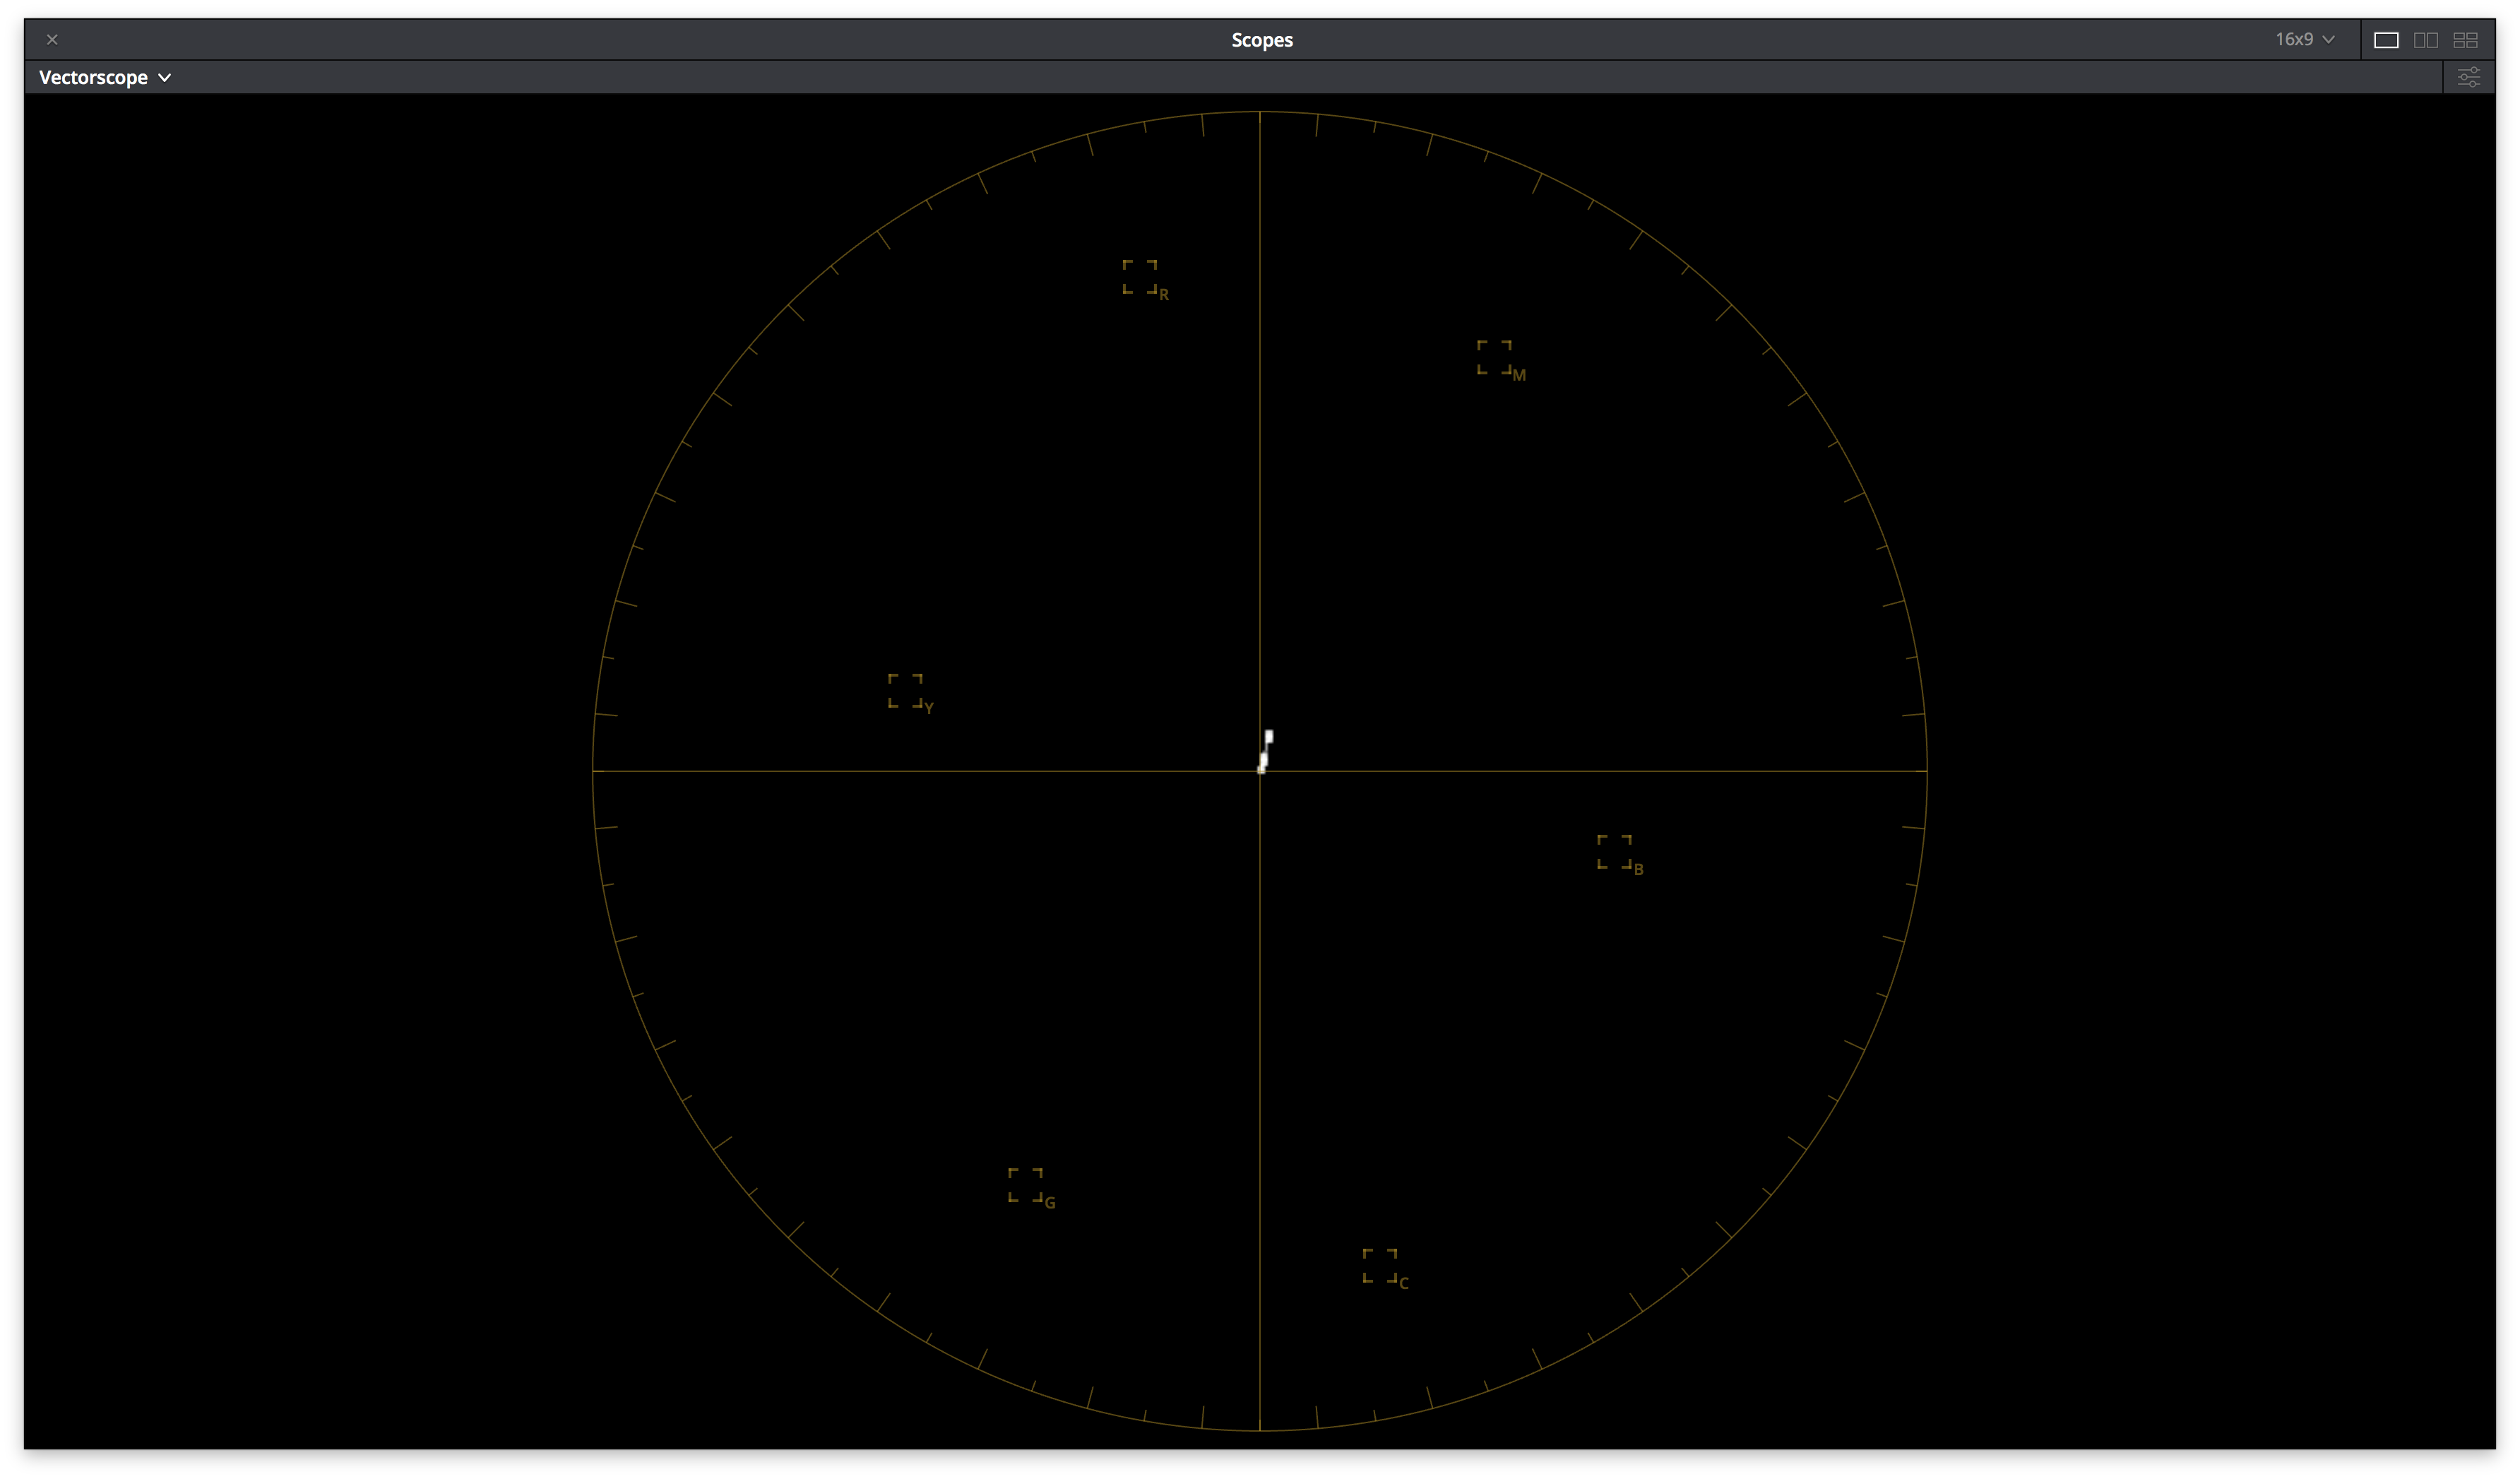
\includegraphics[width=\textwidth]{images/p3dci/p3dci_vectorscope}
            \caption[]%
            {{\small vectorscope}}    
            \label{fig:vect-p3dci}
        \end{subfigure}
        \quad
        \begin{subfigure}[b]{0.475\textwidth}   
            \centering 
            
\includegraphics[width=\textwidth]{images/p3dci/p3dci_image}
            \caption[Projector code values as displayed on a D65 calibrated computer monitor]%
            {{\small Projector code values as displayed on a D65 calibrated computer monitor}}    
            \label{fig:cv-p3dci}
        \end{subfigure}
        \caption[]
        {\small \texttt{\seqsplit{ODT.Academy.P3DCI\_48nits.a1.0.3}} Scope Screenshots} 
        \label{fig:screenshots-p3dci}
    \end{figure*}

\subsection{Test Values}
\label{subsec:testValues-p3dci}

Table \ref{tab:testValues-p3dci} contains test values can be used to confirm the proper monitor setup and ODT combination.  Each of the 9 ACES RGB input values should yield the RGB noted display RGB code values (normalized 0-1, full range) when processed through the \texttt{\seqsplit{ODT.Academy.P3DCI\_48nits.a1.0.3}}. When driving a properly setup display with the noted display RGB code values, the light from the display should measure with the noted CIE xyY colorimetry.  

If the display RGB code values do not match those in the table when using the corresponding input ACES RGB code values, it is likely the wrong ODT is being used.  If the proper display RGB code values are being produced by the ODT, but he measured display colorimetry doesn't match the display xyY code values noted, it is likely the display setup is incorrect.

\begin{table}[ht!]
    \centering
    \begin{tabular}{|l|l|l|l|l|l|l|l|l|l|}
        \hline
        \multicolumn{1}{|c|}{\textbf{Patch}} & \multicolumn{3}{c|}{\textbf{ACES RGB}} & \multicolumn{3}{c|}{\textbf{Display RGB}} & \multicolumn{3}{c|}{\textbf{Display xyY}} \\ \hline
        \textbf{N1} & 1.8233 & 1.8233 & 1.8233 & 0.9243 & 0.8651 & 0.9013 & 0.3217 & 0.3377 & 34.4858 \\ \hline
        \textbf{N2} & 0.2753 & 0.2753 & 0.2753 & 0.5383 & 0.5038 & 0.5249 & 0.3217 & 0.3377 & 8.4552  \\ \hline
        \textbf{N3} & 0.0898 & 0.0898 & 0.0898 & 0.2804 & 0.2625 & 0.2734 & 0.3217 & 0.3377 & 1.5514  \\ \hline
        \textbf{R}  & 0.4689 & 0.1193 & 0.0417 & 0.8046 & 0.2227 & 0.1795 & 0.6413 & 0.3307 & 6.4488  \\ \hline
        \textbf{G}  & 0.339  & 0.8068 & 0.0936 & 0.4335 & 0.8036 & 0.2434 & 0.3046 & 0.624  & 20.8422 \\ \hline
        \textbf{B}  & 0.2162 & 0.133  & 0.8711 & 0.1707 & 0.1503 & 0.8215 & 0.1562 & 0.0692 & 2.3365  \\ \hline
        \textbf{C}  & 0.5187 & 0.9138 & 1.0432 & 0.4332 & 0.8028 & 0.8406 & 0.2269 & 0.3404 & 22.8164 \\ \hline
        \textbf{M}  & 0.58   & 0.2096 & 0.9086 & 0.808  & 0.2134 & 0.8294 & 0.333  & 0.1596 & 8.4349  \\ \hline
        \textbf{Y}  & 0.8237 & 0.9378 & 0.0855 & 0.8654 & 0.8096 & 0.2487 & 0.4338 & 0.5187 & 26.9923 \\ \hline
    \end{tabular}
    \caption[Theatrical DI (P3DCI) - Test Values]{ \texttt{ODT.Academy.P3DCI\_48nits.a1.0.3} Test Values}
    \label{tab:testValues-p3dci}
\end{table}


%%%% Application -- Theatrical Digital Intermediate (P3-D60 Calibrated Projector) %%%% 
\clearpage
\section{Theatrical Digital Intermediate (P3-D60 Calibrated Projector)}
\label{sec:ot-app-p3d60}

\subsection{Summary}
\label{subsec:summary-p3d60}

It is common in the digital intermediate process (DI) to color correct
motion pictures and episodic television shows while displaying the
images using a DCI compliant digital cinema projector. DCI compliant
digital cinema projectors have a simplified setup using a projector
configuration file (PCF) that contains all the relevant projector
settings and can often be loaded at the press of a button. The
recommended PCF to be used with digital cinema projectors and ACES-based
workflows is the ``P3-D60'' PCF \textbf{(add link)}. Using this PCF, the
projector will be configured such that equal red, green, and blue
projector code values will produce the chromaticity x=0.32168 y=0.33767
(aka D60). With the projector configured in this manner it is
recommended that ACES ODT with the transformID
\texttt{\seqsplit{ODT.Academy.P3D60\_48nits.a1.0.3}} be used.

\subsection{Projector Setup}
\label{subsec:setup-p3d60}

\begin{table}[ht!]
    \centering
        \begin{tabular}{|p{1.25in}|p{3in}|}
            \hline
            \textbf{Parameter} & \textbf{Setting} \\ \hline
            PCF & P3D60(RGB 4:4:4 Full Range, P3 Primaries, D60 white point, 48 nit max Luminance) \\ \hline
            Viewing Environment & Dark \\ \hline
            Bit Depth & 12-bit \\ \hline 
    \end{tabular}
    \caption[Theatrical DI (P3D60) - Projector Setup]{\small P3-D60 Projector Setup} 
    \label{tab:setup-p3d60}
\end{table}

\subsection{Best ODT for application} 
\label{subsec:bestODT-p3d60}

\begin{table}[ht!]
    \centering
    \begin{tabular}{|p{1.5in}|p{3in}|}
        \hline
        \textbf{Simple Name} & \textbf{TransformID} \\ \hline
        ACES 1.0 Output - P3-D60 & \texttt{\seqsplit{ODT.Academy.P3D60\_48nits.a1.0.3}} \\ \hline
    \end{tabular}
    \caption[Theatrical DI (P3D60) - Best ODT]{\small P3-D60 Best ODT} 
    \label{tab:bestODT-p3d60}
\end{table}

\subsection{Notes}
\label{subsec:notes-p3d60}

The ``P3-D60'' PCF is not typically included by the manufacturer by
default in most digital cinema projectors. It must be downloaded and
installed in the projector using the appropriate projector configuration
software (e.g.~DCP Librarian). Once the PCF is installed and activated
neutral ACES values sent through the the
\texttt{\seqsplit{ODT.Academy.P3D60\_48nits.a1.0.3}} transform will produce equal
red, green and blue projector code values, will have equal levels on the
waveform, will land in the middle of the vector scope, will appear
neutral on a D65 calibrated computer monitor, and will produce the
chromaticity x=0.32168 y=0.33767 (aka D60) on the projection screen.
(Figure \ref{fig:acesSource-p3d60}, \ref{fig:hist-p3d60}, \ref{fig:parade-p3d60}, \ref{fig:wf-p3d60}, \ref{fig:vect-p3d60})

Often the resulting projector code values are saved into a file and
converted using specialized tools (e.g. Clipster) into DCDMs and/or a
DPC for distribution. It is important to note that many conversion tools
assume that equal red, green, and blue projector code values are
intended to produce a chromaticity of x=0.3140 y=0.3510 on the screen.
Converting the projector code values from
\texttt{\seqsplit{ODT.Academy.P3D60\_48nits.a1.0.3}} using such tools will result
in incorrect DCDM and/or DCP files. The tools must explicitly be capable
of converting projector code values where equal red, green, and blue
projector code values are intended to produce a chromaticity x=0.32168
y=0.33767 (aka D60) on the screen.

When using the correct projector setup and corresponding ODT, the image
on the projector screen will match nearly exactly in Application \ref{sec:ot-app-p3dci} and
Application \ref{sec:ot-app-p3d60}.

    \begin{figure*}[ht!]
        \centering
        \begin{subfigure}[b]{0.475\textwidth}
            \centering
            
\includegraphics[width=\textwidth]{images/aces}
            \caption[Source ACES Image]%
            {{\small ACES Image}}    
            \label{fig:acesSource-p3d60}
        \end{subfigure}
        \hfill
        \begin{subfigure}[b]{0.475\textwidth}  
            \centering 
            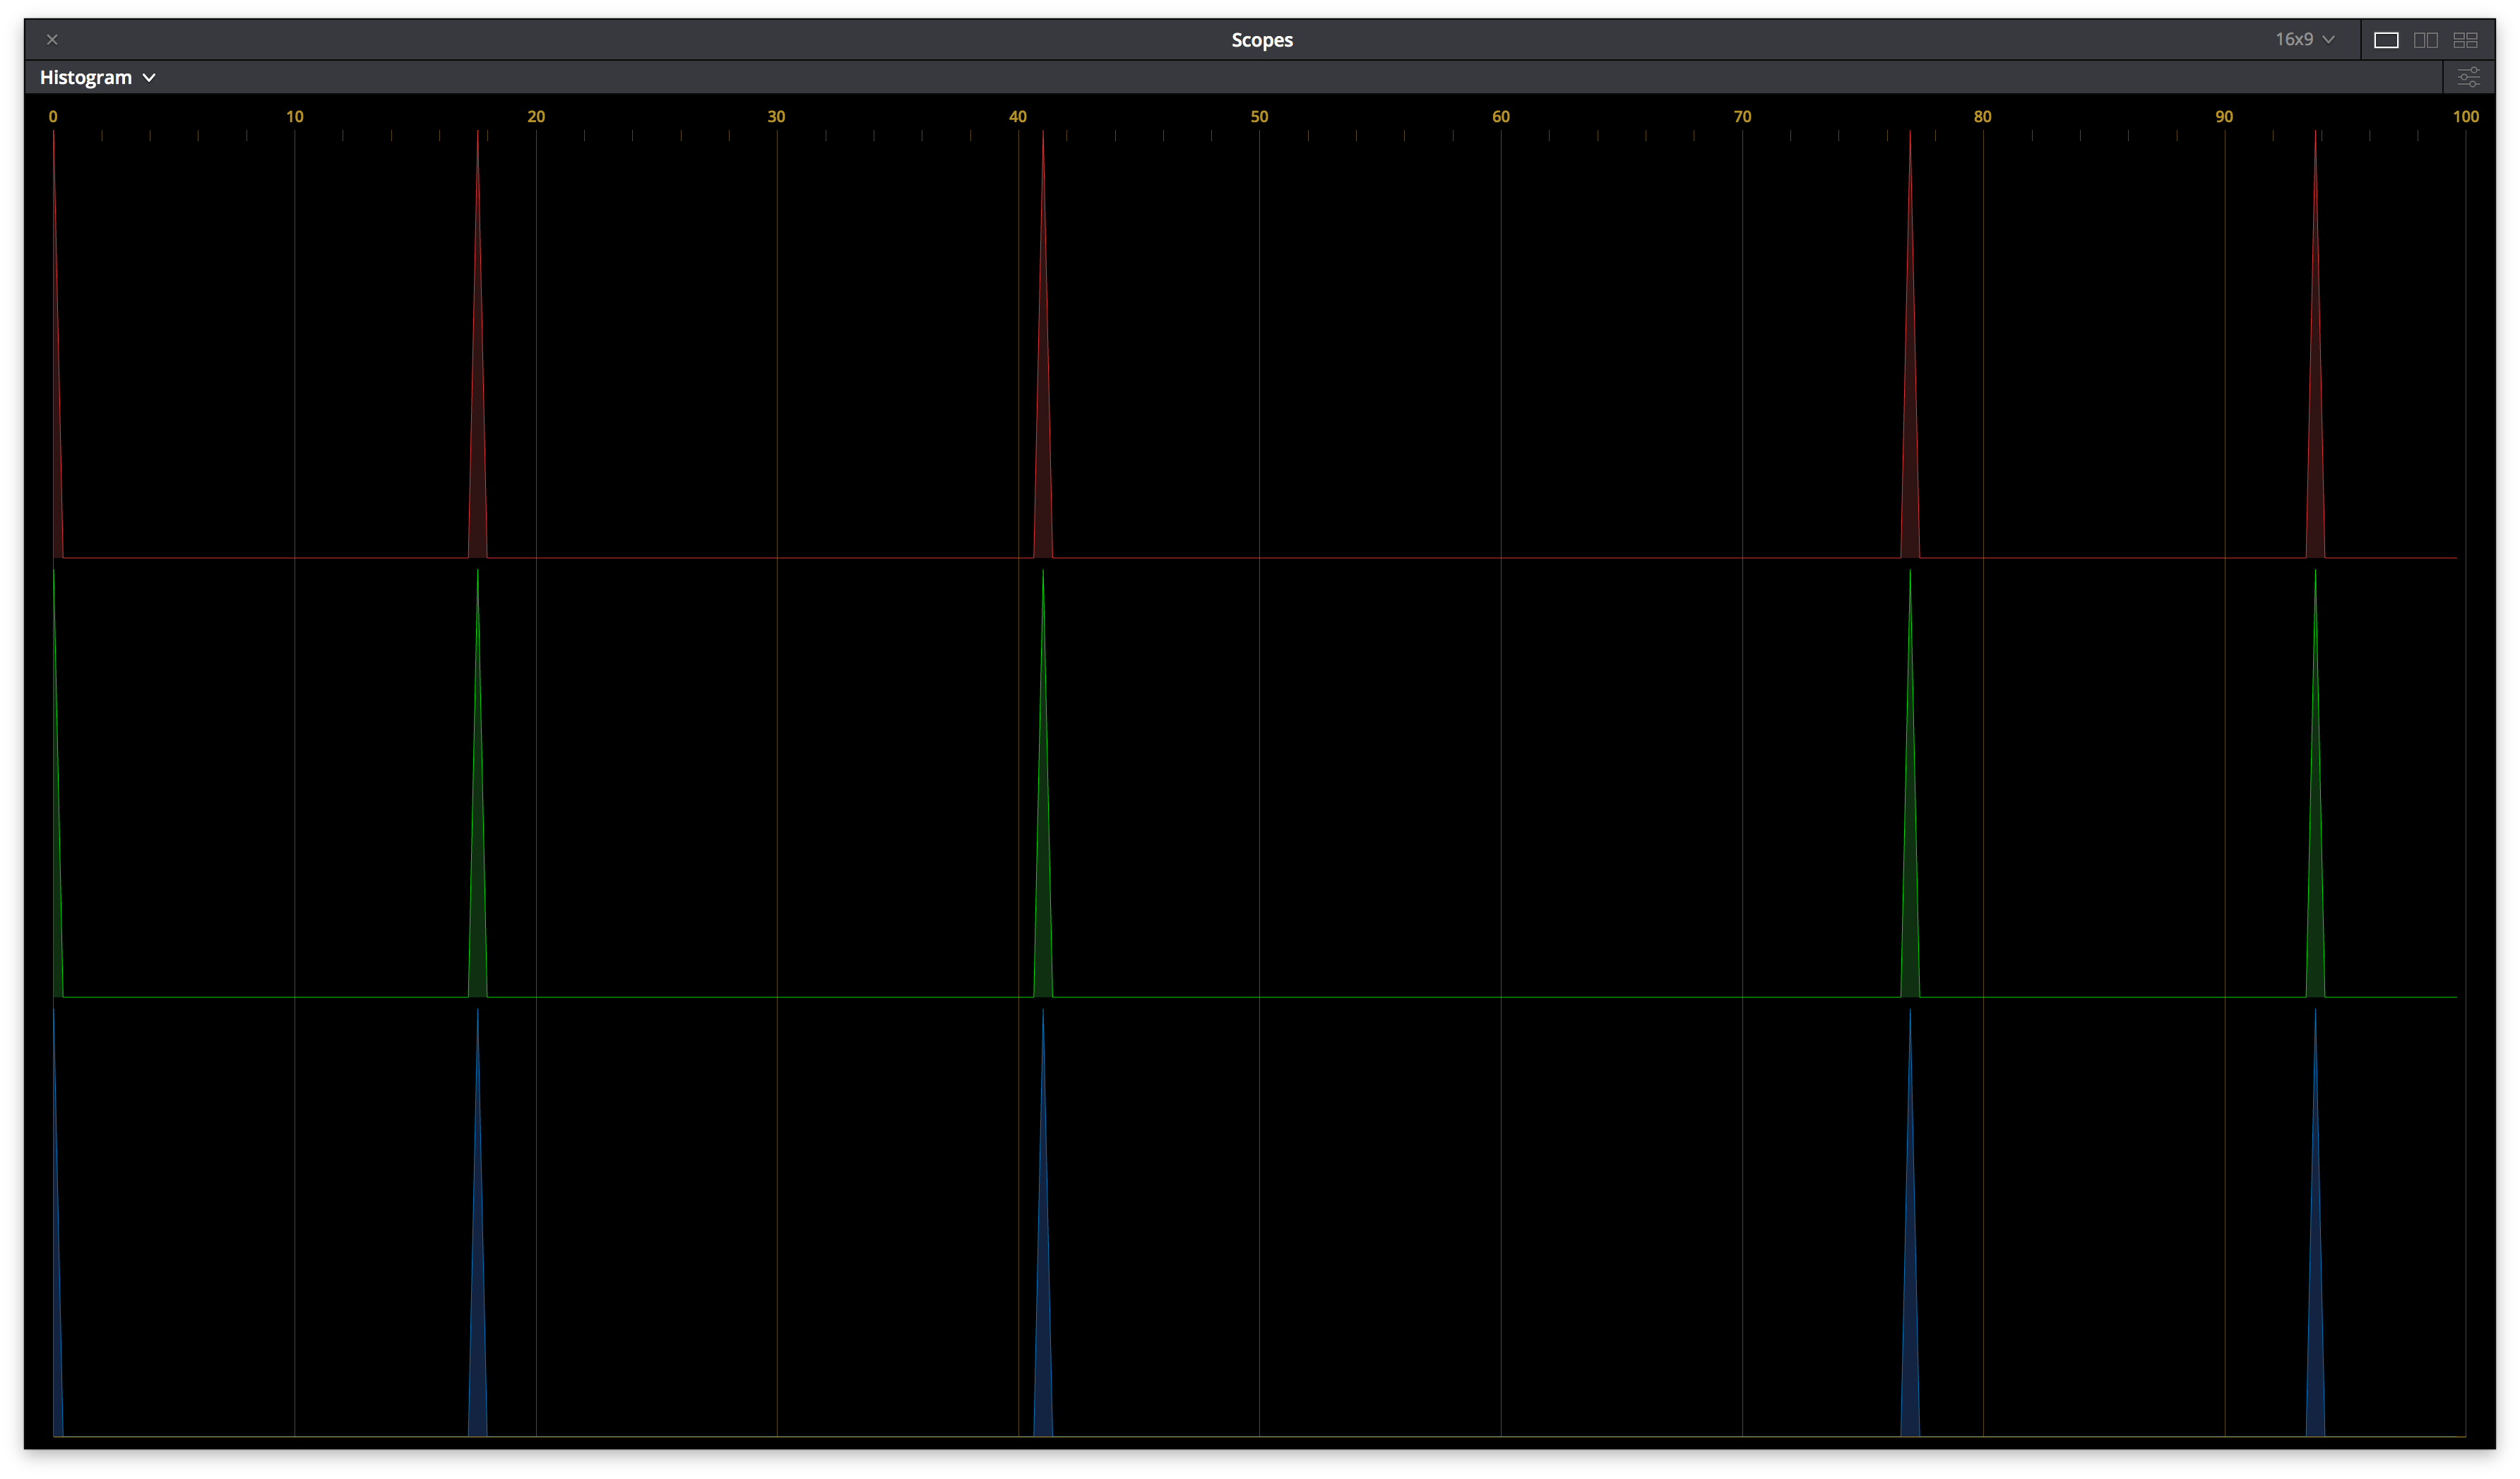
\includegraphics[width=\textwidth]{images/p3d60/p3d60_histogram}
            \caption[Histogram]%
            {{\small Histogram}}    
            \label{fig:hist-p3d60}
        \end{subfigure}
        \vskip\baselineskip
        \begin{subfigure}[b]{0.475\textwidth}   
            \centering 
            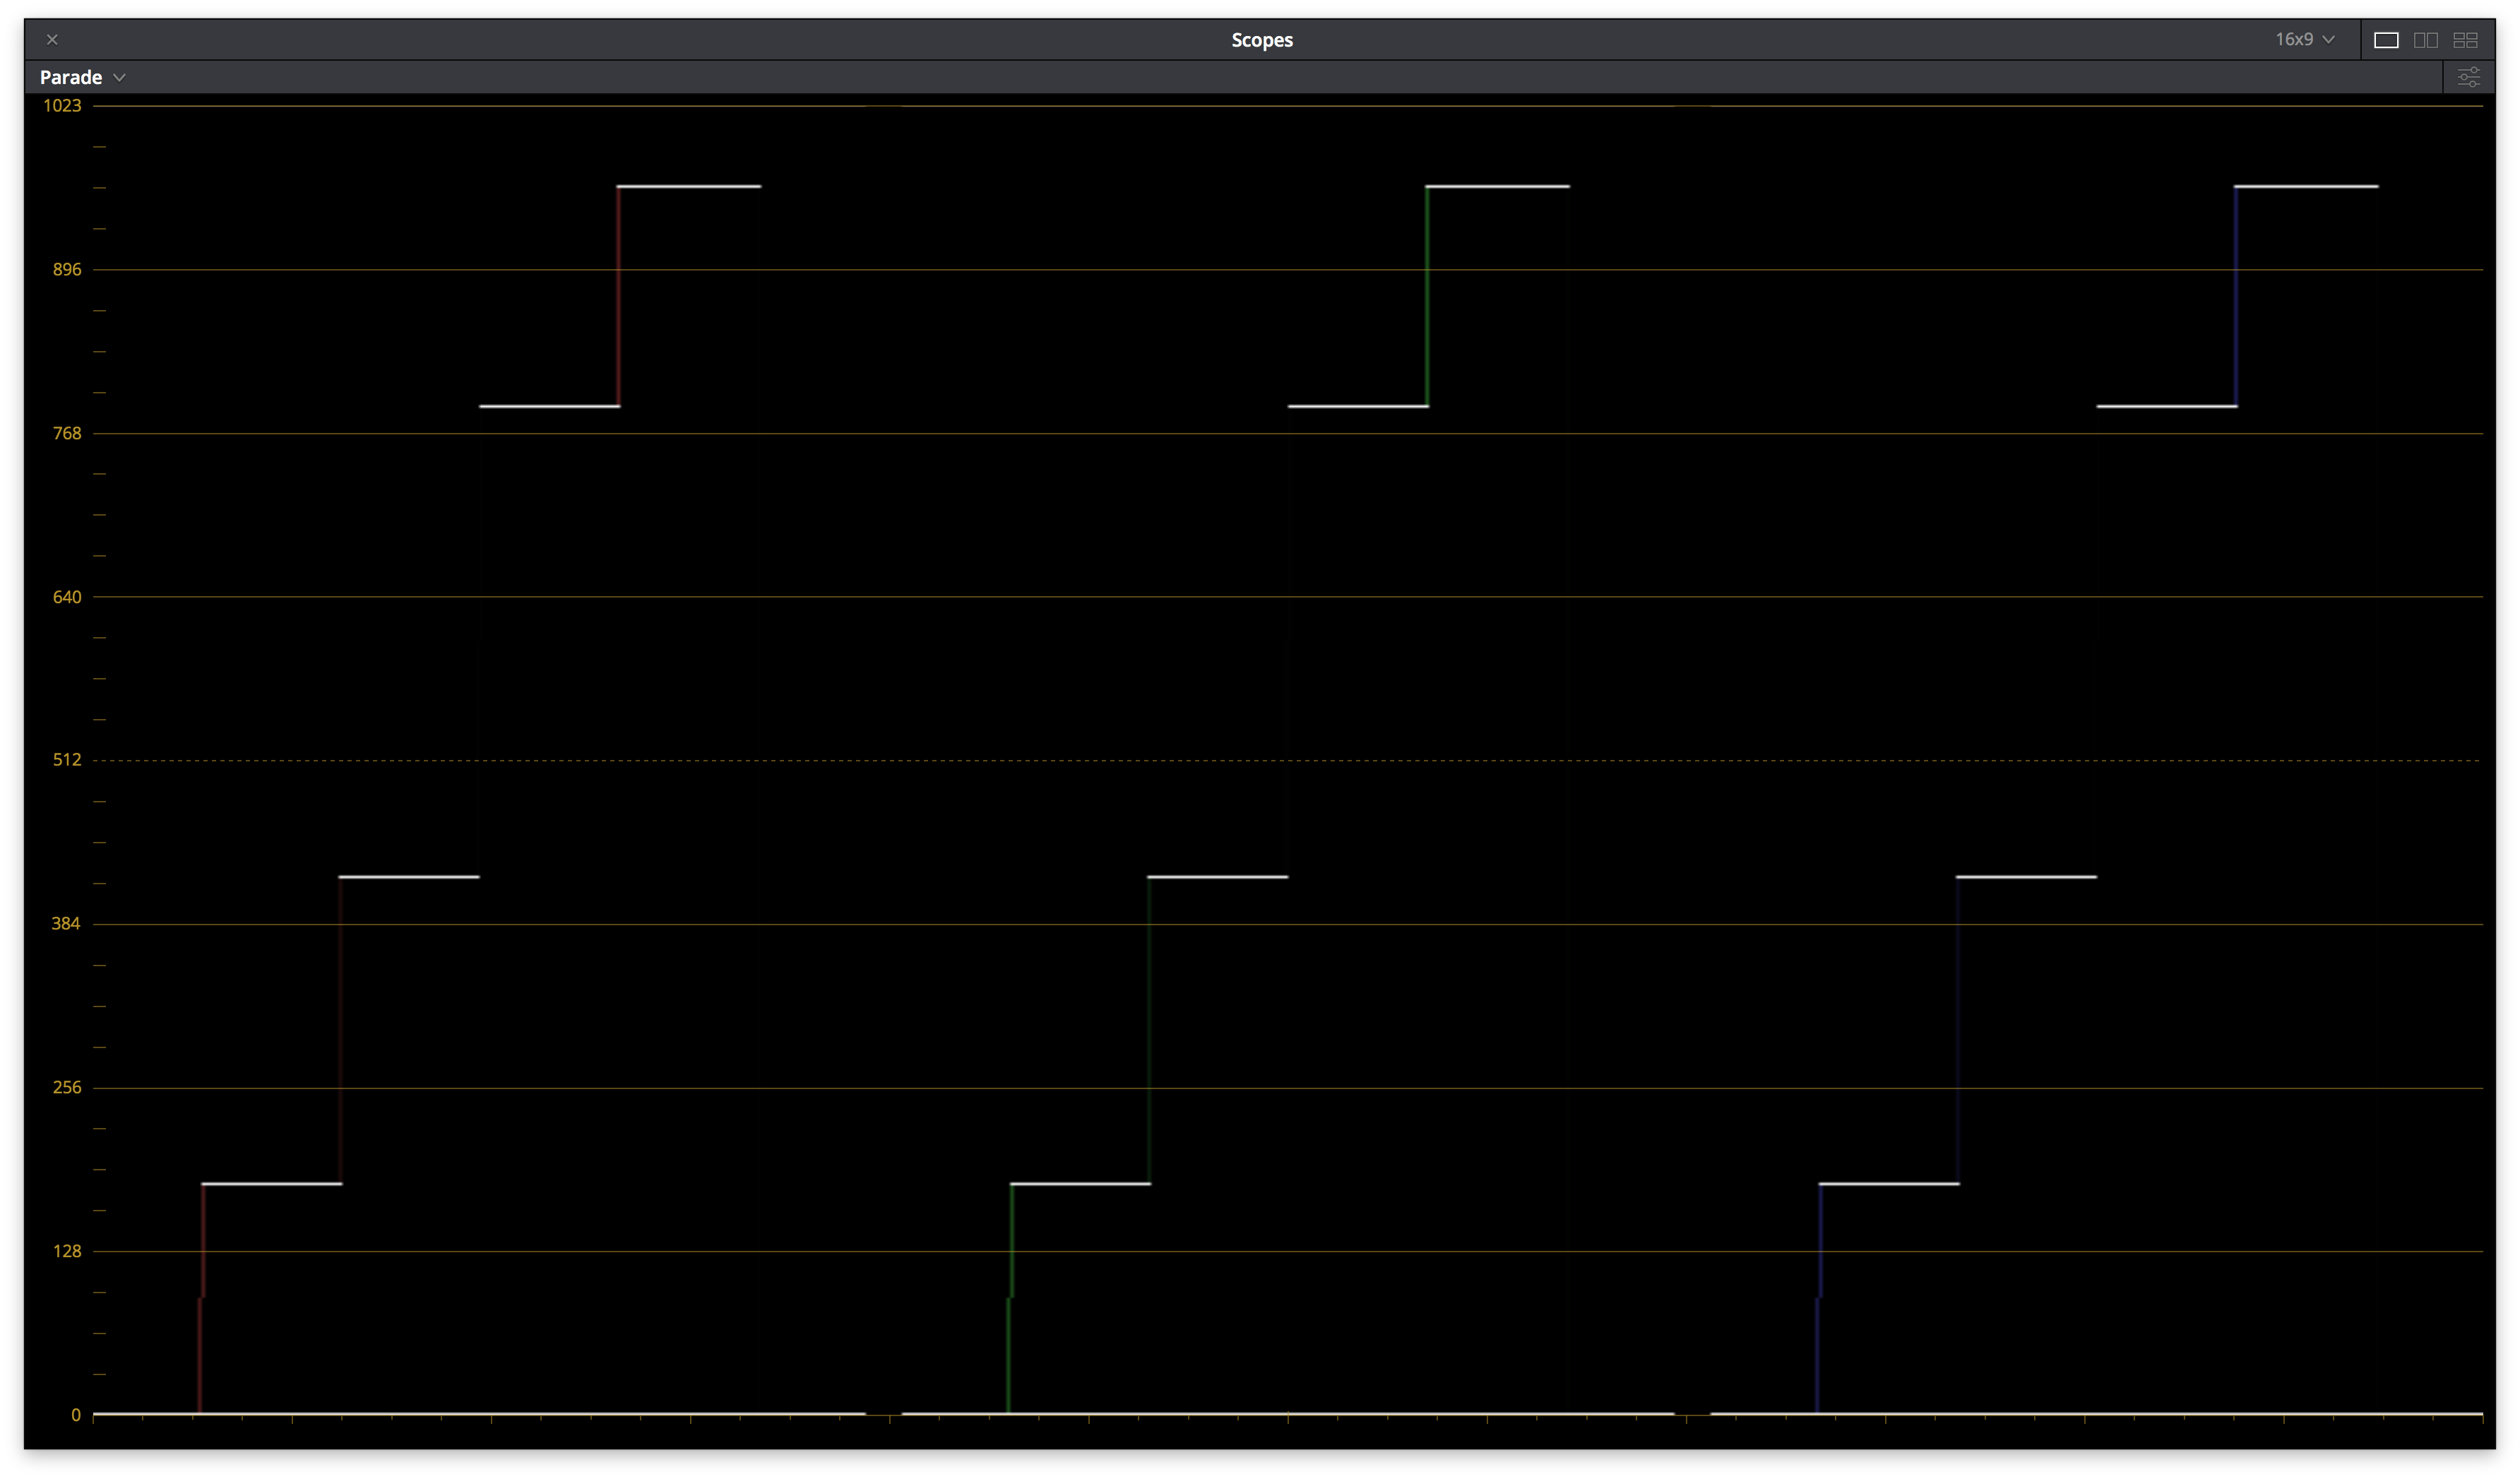
\includegraphics[width=\textwidth]{images/p3d60/p3d60_parade}
            \caption[Parade]%
            {{\small Parade}}    
            \label{fig:parade-p3d60}
        \end{subfigure}
        \quad
        \begin{subfigure}[b]{0.475\textwidth}   
            \centering 
            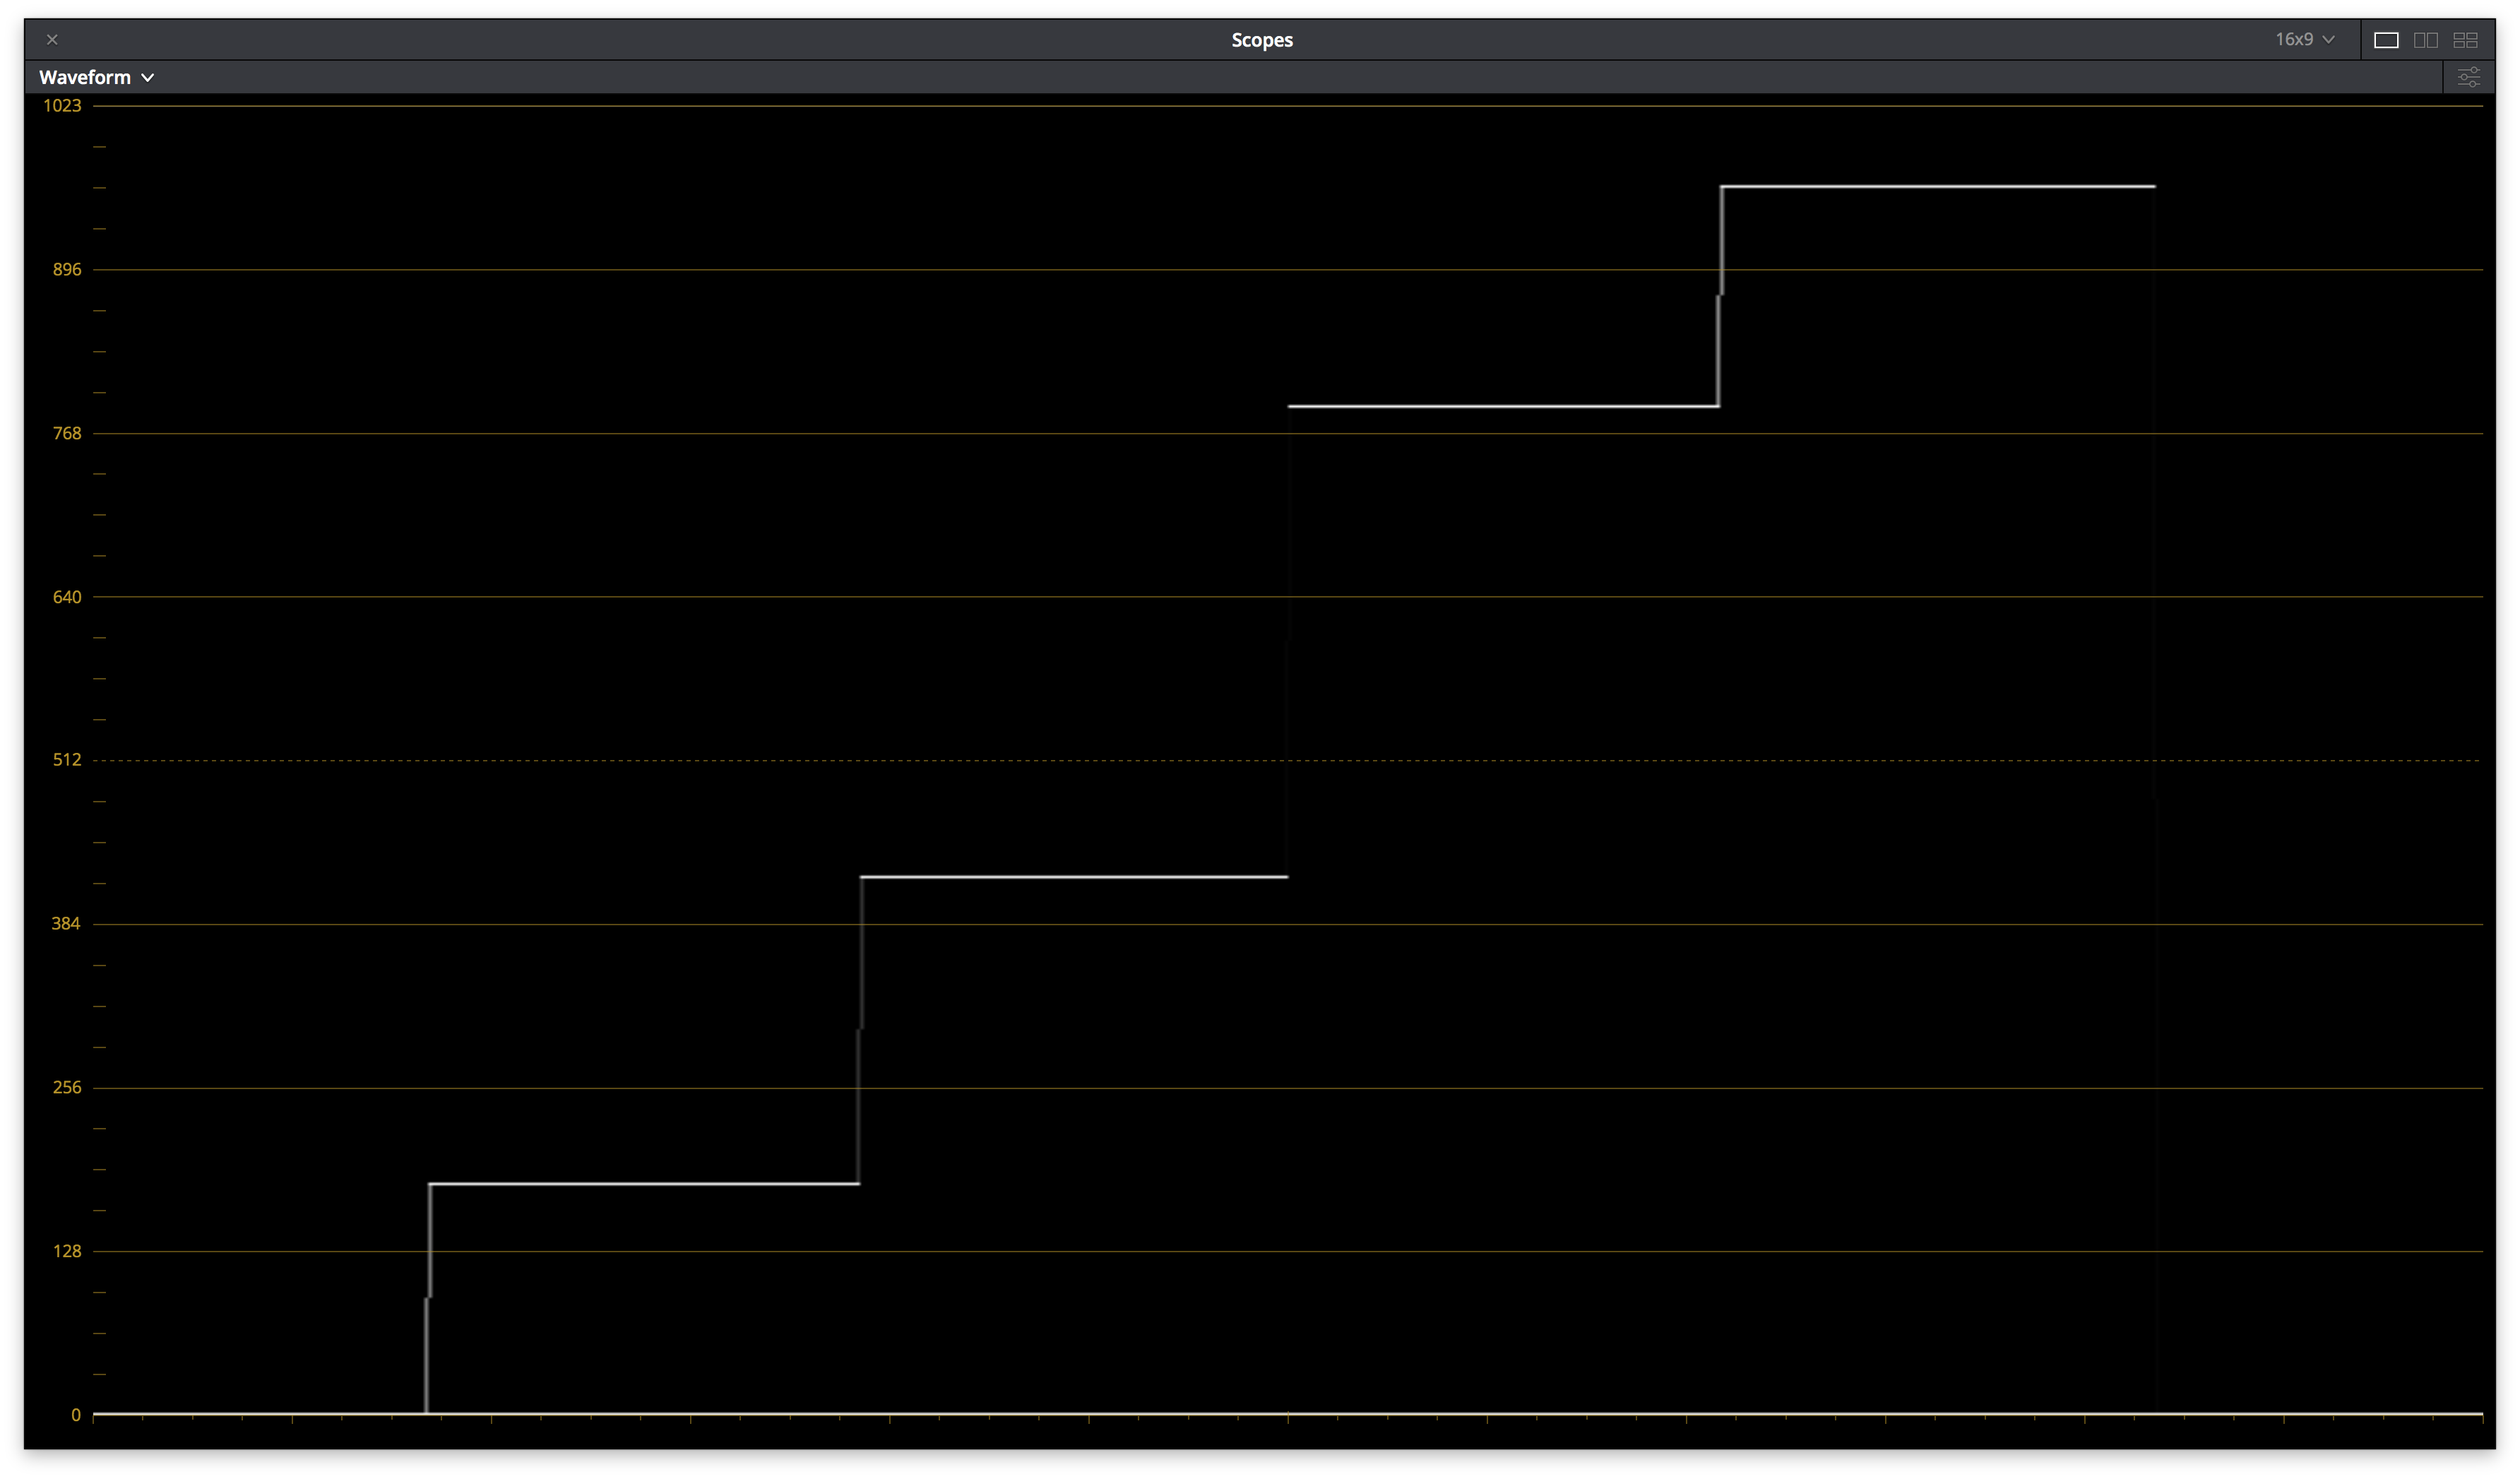
\includegraphics[width=\textwidth]{images/p3d60/p3d60_waveform}
            \caption[]%
            {{\small Waveform}}    
            \label{fig:wf-p3d60}
        \end{subfigure}
        \begin{subfigure}[b]{0.475\textwidth}   
            \centering 
            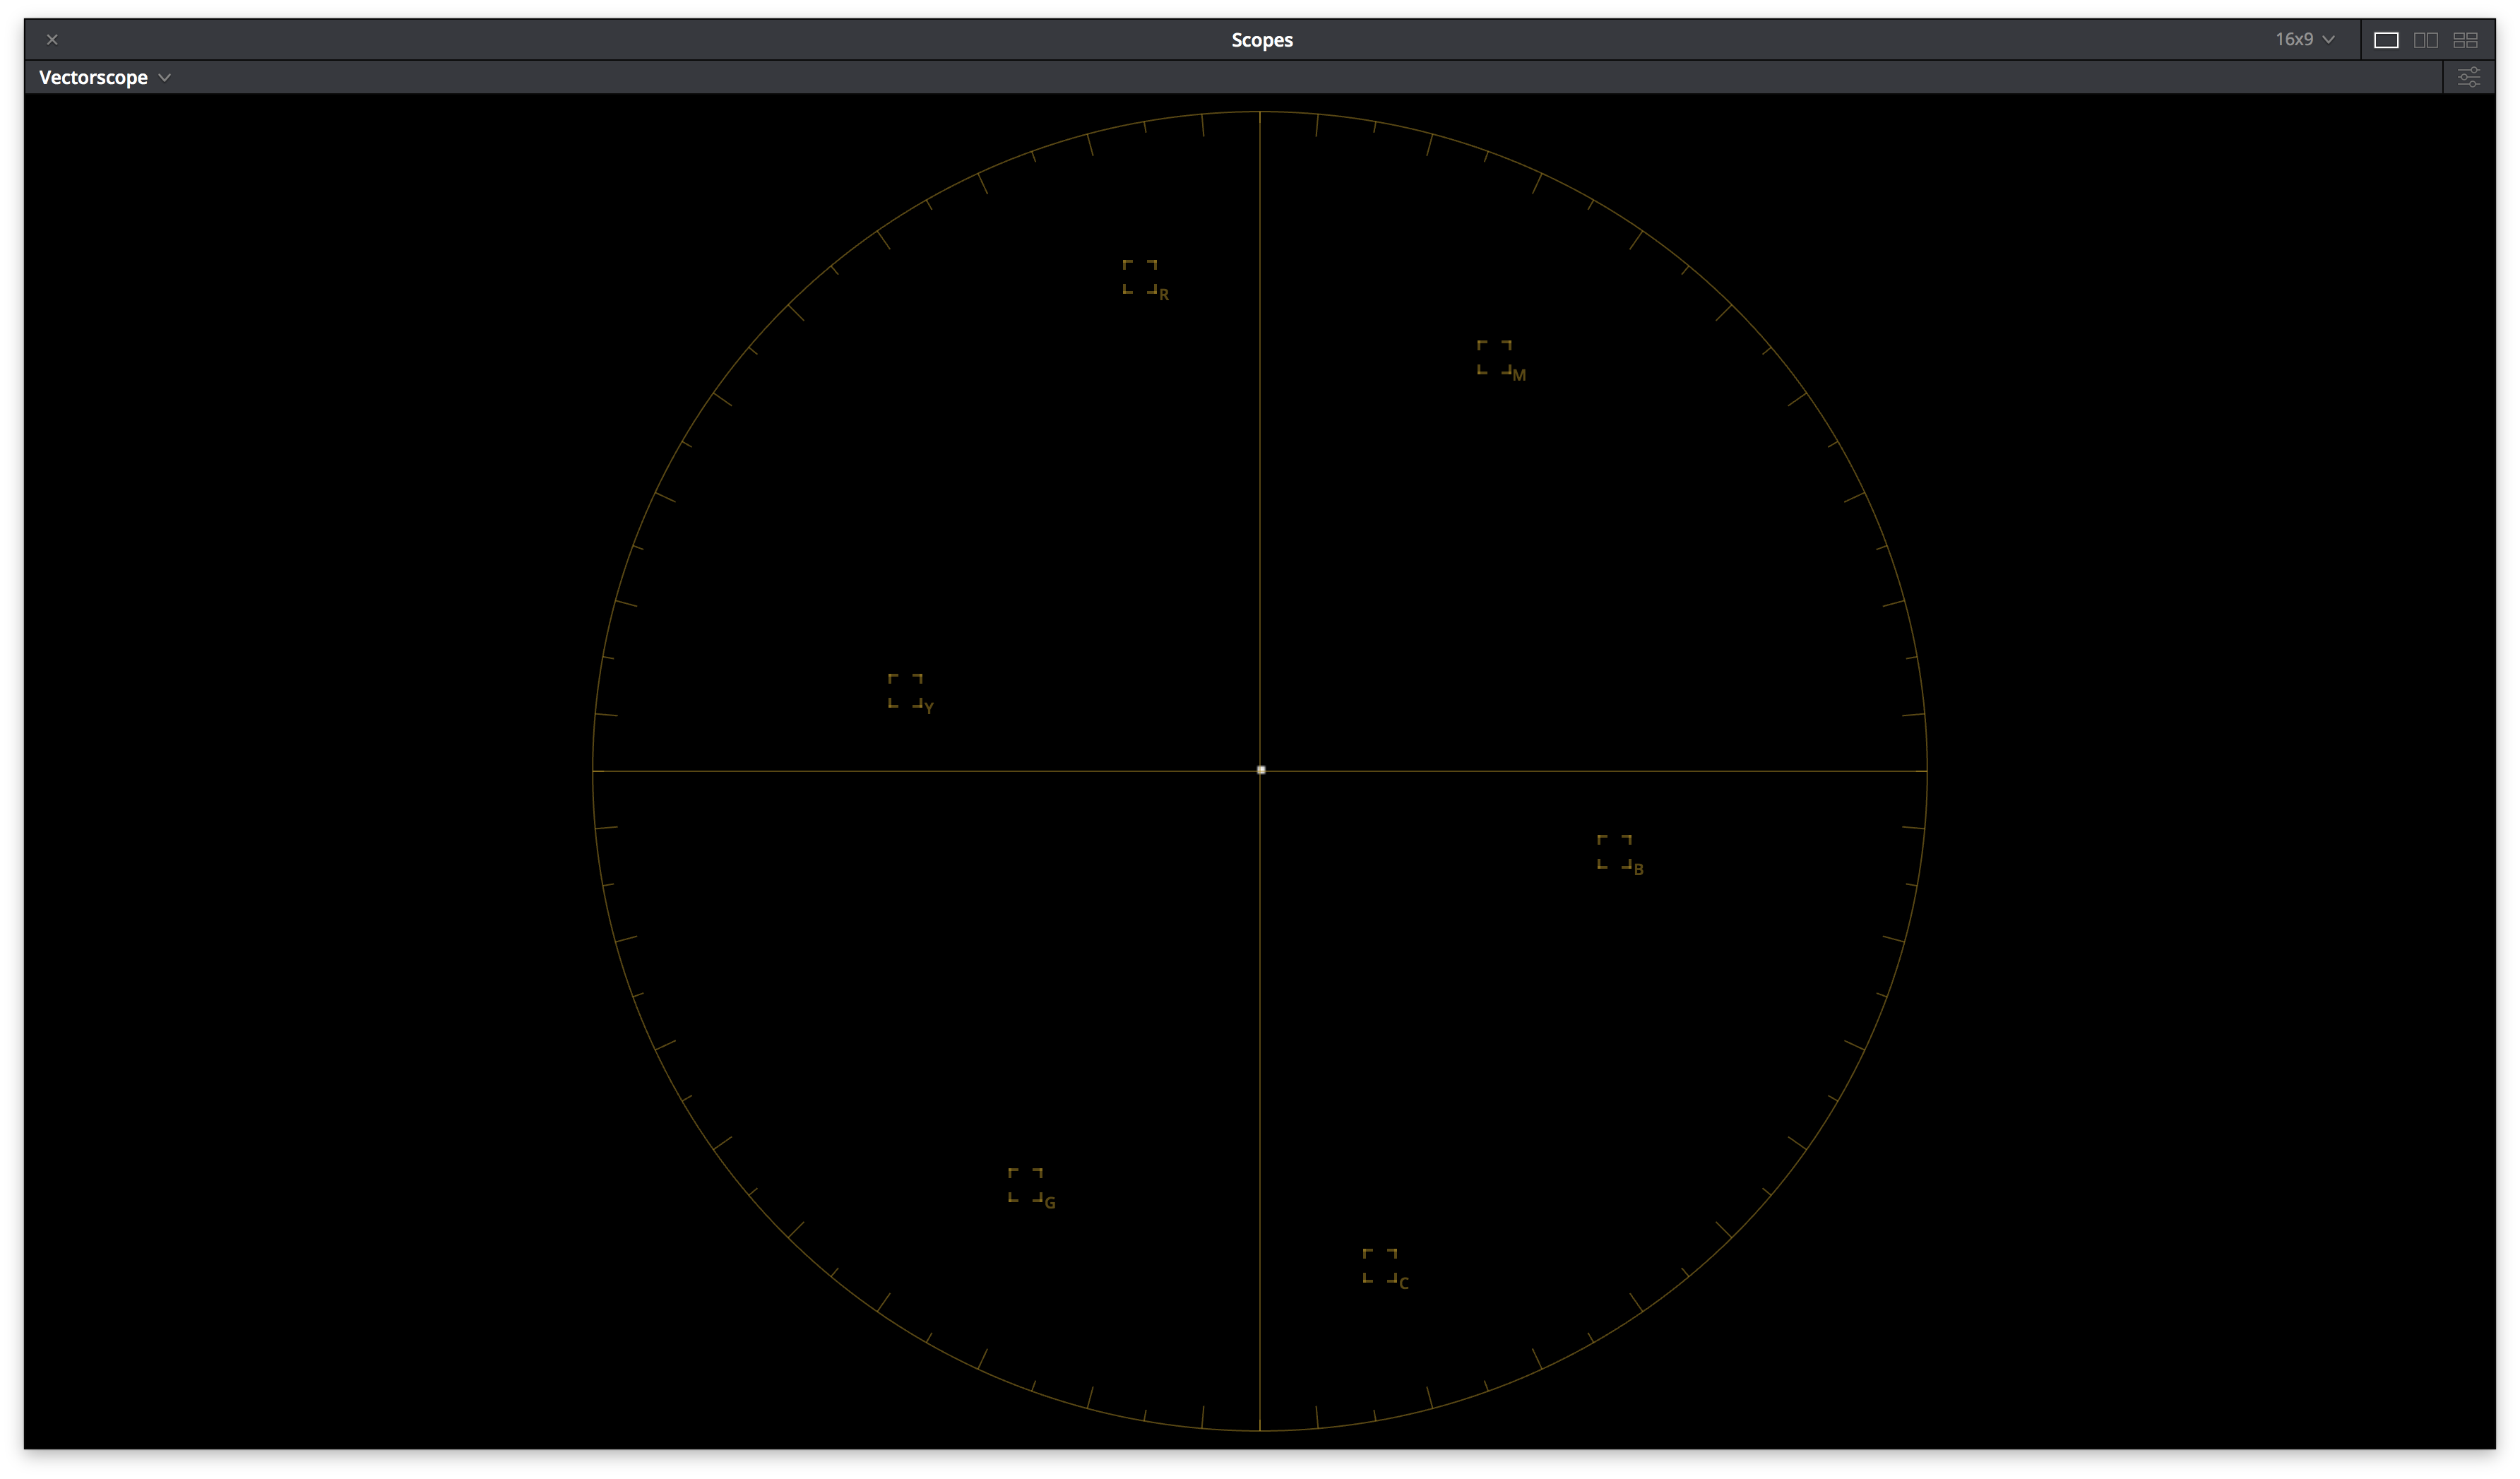
\includegraphics[width=\textwidth]{images/p3d60/p3d60_vectorscope}
            \caption[]%
            {{\small vectorscope}}    
            \label{fig:vect-p3d60}
        \end{subfigure}
        \quad
        \begin{subfigure}[b]{0.475\textwidth}   
            \centering 
            
\includegraphics[width=\textwidth]{images/p3d60/p3d60_image.png}
            \caption[Projector code values as displayed on a D65 calibrated computer monitor]%
            {{\small Projector code values as displayed on a D65 calibrated computer monitor}}    
            \label{fig:cv-p3d60}
        \end{subfigure}
        \caption[]
        {\small \texttt{ODT.Academy.P3D60\_48nits.a1.0.3} Scope Screenshots} 
        \label{fig:screenshots-p3d60}
    \end{figure*}

\subsection{Test Values}
\label{subsec:testValues-p3d60}

Table \ref{tab:testValues-p3d60} contains test values can be used to confirm the proper monitor setup and ODT combination.  Each of the 9 ACES RGB input values should yield the RGB noted display RGB code values (normalized 0-1, full range) when processed through the \texttt{\seqsplit{ODT.Academy.P3D60\_48nits.a1.0.3}}. When driving a properly setup display with the noted display RGB code values, the light from the display should measure with the noted CIE xyY colorimetry.  

If the display RGB code values do not match those in the table when using the corresponding input ACES RGB code values, it is likely the wrong ODT is being used.  If the proper display RGB code values are being produced by the ODT, but he measured display colorimetry doesn't match the display xyY code values noted, it is likely the display setup is incorrect.

\begin{table}[ht!]
    \centering
    \begin{tabular}{|l|l|l|l|l|l|l|l|l|l|}
        \hline
        \multicolumn{1}{|c|}{\textbf{Patch}} & \multicolumn{3}{c|}{\textbf{ACES RGB}} & \multicolumn{3}{c|}{\textbf{Display RGB}} & \multicolumn{3}{c|}{\textbf{Display xyY}} \\ \hline
        \textbf{N1} & 1.8233 & 1.8233 & 1.8233 & 0.9056 & 0.9056 & 0.9056 & 0.3217 & 0.3377 & 37.0944 \\ \hline
        \textbf{N2} & 0.2753 & 0.2753 & 0.2753 & 0.5209 & 0.5209 & 0.5209 & 0.3217 & 0.3377 & 8.8075  \\ \hline
        \textbf{N3} & 0.0898 & 0.0898 & 0.0898 & 0.2714 & 0.2714 & 0.2714 & 0.3217 & 0.3377 & 1.6161  \\ \hline
        \textbf{R}  & 0.4689 & 0.1193 & 0.0417 & 0.7786 & 0.2302 & 0.1781 & 0.6413 & 0.3307 & 6.7175  \\ \hline
        \textbf{G}  & 0.339  & 0.8068 & 0.0936 & 0.4184 & 0.8322 & 0.2411 & 0.3042 & 0.6246 & 21.7918 \\ \hline
        \textbf{B}  & 0.2162 & 0.133  & 0.8711 & 0.1647 & 0.1553 & 0.816  & 0.1562 & 0.0692 & 2.4372  \\ \hline
        \textbf{C}  & 0.5187 & 0.9138 & 1.0432 & 0.4174 & 0.8317 & 0.8371 & 0.2263 & 0.3398 & 23.8751 \\ \hline
        \textbf{M}  & 0.58   & 0.2096 & 0.9086 & 0.7819 & 0.2206 & 0.8243 & 0.3325 & 0.1593 & 8.7918  \\ \hline
        \textbf{Y}  & 0.8237 & 0.9378 & 0.0855 & 0.8392 & 0.8399 & 0.2459 & 0.4336 & 0.5192 & 28.3358 \\ \hline
        \end{tabular}
        \caption[Theatrical DI (P3D60) - Test Values]{\texttt{ODT.Academy.P3D60\_48nits.a1.0.3} Test Values}
        \label{tab:testValues-p3d60}
\end{table}

%%%% Application - Theatrical On-Set Preview (Rec.709 SDR Reference Monitor) %%%% 
\clearpage
\section{Theatrical On-Set Preview (Rec.709 SDR Reference Monitor)}
\label{sec:ot-app-rec709d60sim}

\subsection{Summary}
\label{subsec:summary-rec709d60sim}

In theatrical workflows it is often desirable to preview the final look of the image on set as it is expected to appear during final color grading and mastering.  Using ACES based workflows it is likely the default chromaticity of neutrals will be x=0.32168 y=0.33767 (aka D60) on the DI projection screen regardless of the projector's calibration white point.  In order to properly preview this on-set it is recommended a Rec.709 SDR reference monitor with a calibration white point of CIE x=0.3127 y=0.3290 (aka D65) be used in conjunction with the ACES Output Transform \texttt{\seqsplit{ODT.Academy.Rec709\_D60sim\_100nits\_dim.a1.0.3}}.

\subsection{Display Setup}
\label{subsec:setup-rec709d60sim}

\begin{table}[ht!]
    \centering
        \begin{tabular}{|p{1.25in}|p{3in}|}
            \hline
            \textbf{Parameter} & \textbf{Setting} \\ \hline
            Max Luminance & 100 nits \\ \hline
            Display White Point & D65 \\ \hline
            Primaries & Rec.709  \\ \hline
            EOTF & BT.1886 \\ \hline
            Viewing Environment & dim \\ \hline
            Signal & RGB 4:4:4 (Full range or Legal Range) \\ \hline
            Bit Depth & 10 or 12-bit \\ \hline 
    \end{tabular}
    \caption[Theatrical On-Set Preview - Display Setup]{\small Rec.709 Display Setup} 
    \label{tab:setup-rec709d60sim}
\end{table}

\subsection{Best ODT for application} 
\label{subsec:bestODT-rec709d60sim}

\begin{table}[ht!]
    \centering
    \begin{tabular}{|p{2.2in}|p{3.6in}|}
        \hline
        \textbf{Simple Name} & \textbf{TransformID} \\ \hline
        ACES 1.0 Output - Rec.709 (D60 sim.) & \texttt{\seqsplit{ODT.Academy.Rec709\_D60sim\_100nits\_dim.a1.0.3}} \\ \hline
    \end{tabular}
    \caption[Theatrical On-Set Preview - Best ODT]{\small Best Theatrical On-Set Preview ODT} 
    \label{tab:bestODT-rec709d60sim}
\end{table}

\subsection{Notes}
\label{subsec:notes-rec709d60sim}

Using a Rec.709 SDR reference monitor with a calibration white point of D65 in in conjunction with the ACES Output Transform \texttt{\seqsplit{ODT.Academy.Rec709\_D60sim\_100nits\_dim.a1.0.3}} will cause 

Using a Rec.709 SDR reference monitor with a calibration white point of D65 will cause
equal red, green, and blue display code values to produce the
chromaticity x=0.3127 y=0.3290 on the display screen. However, the
\texttt{\seqsplit{ODT.Academy.Rec709\_D60sim\_100nits\_dim.a1.0.3}} transform is configured such that neutral ACES source file values (ACES R=G=B) will produce non-equal
display code values. The chromaticity of produced on screen by those
non-equal projector code values will be x=0.32168 y=0.33767 (aka D60).  This is intentional and designed such that the image appearance on the on-set Rec.709 SDR reference monitor will mimic that of the final image displayed in DI mastering.

It's important to note that the image on projection screen may look less blue then some video based workflows. This will also be reflected on the color
corrector scopes when neutral ACES values sent through the
\texttt{\seqsplit{ODT.Academy.Rec709\_D60sim\_100nits\_dim.a1.0.3}} transform. (Figure \ref{fig:acesSource-rec709_d60sim}, \ref{fig:hist-rec709_d60sim}, \ref{fig:parade-rec709_d60sim}, \ref{fig:wf-rec709_d60sim}, \ref{fig:vect-rec709_d60sim}) For instance,
neutral ACES values processed through
\texttt{\seqsplit{ODT.Academy.Rec709\_D60sim\_100nits\_dim.a1.0.3}} will not have equal levels on
the waveform, nor will they land in the middle of the vector scope. This behavior was intentional. The image may also
have a slightly warm cast on a computer monitor such as the one
used for the color corrector user interface if that monitor is
calibrated to a D65 white point when compared to images generated using some traditional video workflows. (Figure \ref{fig:cv-p3dci}) In the ACES system, the behavior of mimicking the default DI look in the on-set environment is known as ``D60 sim''. Due to this ``D60 sim'' behavior the maximum output screen luminance of neutral ACES values will be
slightly less than the maximum luminance produced by display code
values red = 1, green = 1, blue = 1 (e.g.~100 nits).

When using the correct Rec.709 reference display setup and corresponding ODT, the image
on the projector screen will have a similar appearance to that of Application \ref{sec:ot-app-p3dci} and Application \ref{sec:ot-app-p3d60}.  However, the images will not measure exactly the same due the fact the Rec.709 reference display's max luminance is 100 nits vs 48 nits in DI, and the \texttt{\seqsplit{ODT.Academy.Rec709\_D60sim\_100nits\_dim.a1.0.3}} compensates for a dim viewing environment.

    \begin{figure*}[ht!]
        \centering
        \begin{subfigure}[b]{0.475\textwidth}
            \centering
            
\includegraphics[width=\textwidth]{images/aces}
            \caption[Source ACES Image]%
            {{\small ACES Image}}    
            \label{fig:acesSource-rec709_d60sim}
        \end{subfigure}
        \hfill
        \begin{subfigure}[b]{0.475\textwidth}  
            \centering 
            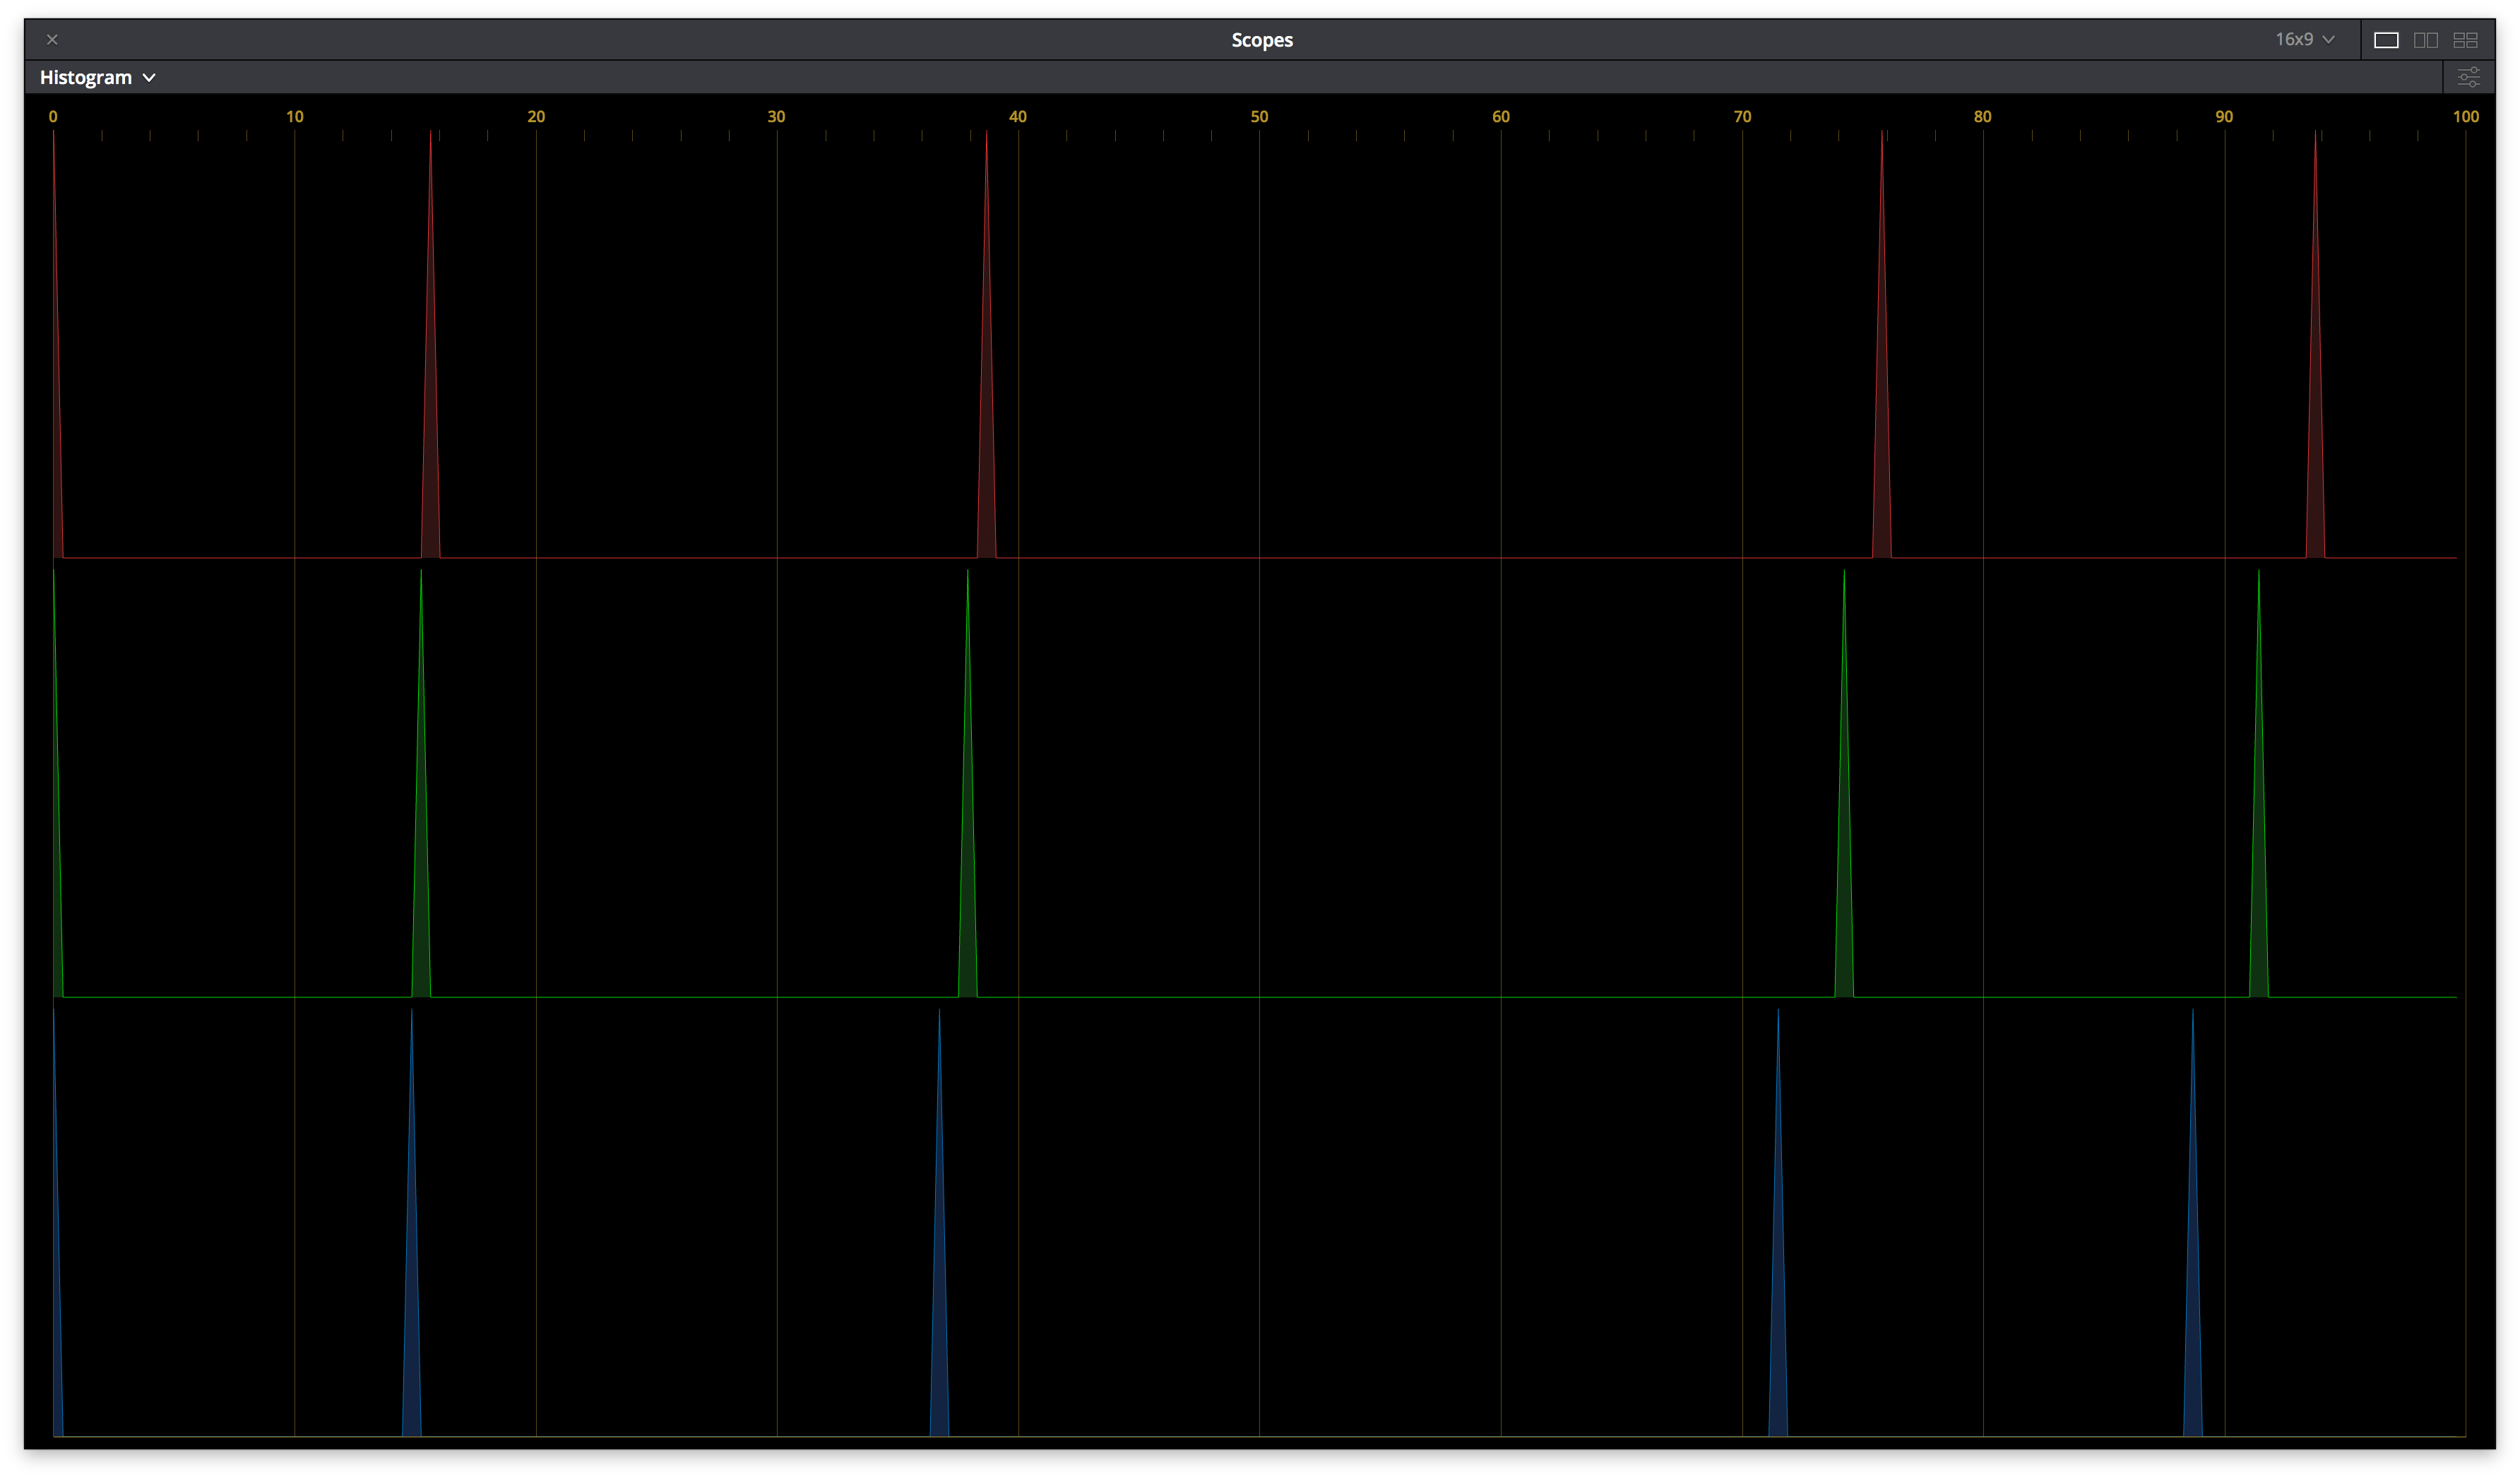
\includegraphics[width=\textwidth]{images/rec709_d60sim/rec709_d60sim_histogram}
            \caption[Histogram]%
            {{\small Histogram}}    
            \label{fig:hist-rec709_d60sim}
        \end{subfigure}
        \vskip\baselineskip
        \begin{subfigure}[b]{0.475\textwidth}   
            \centering 
            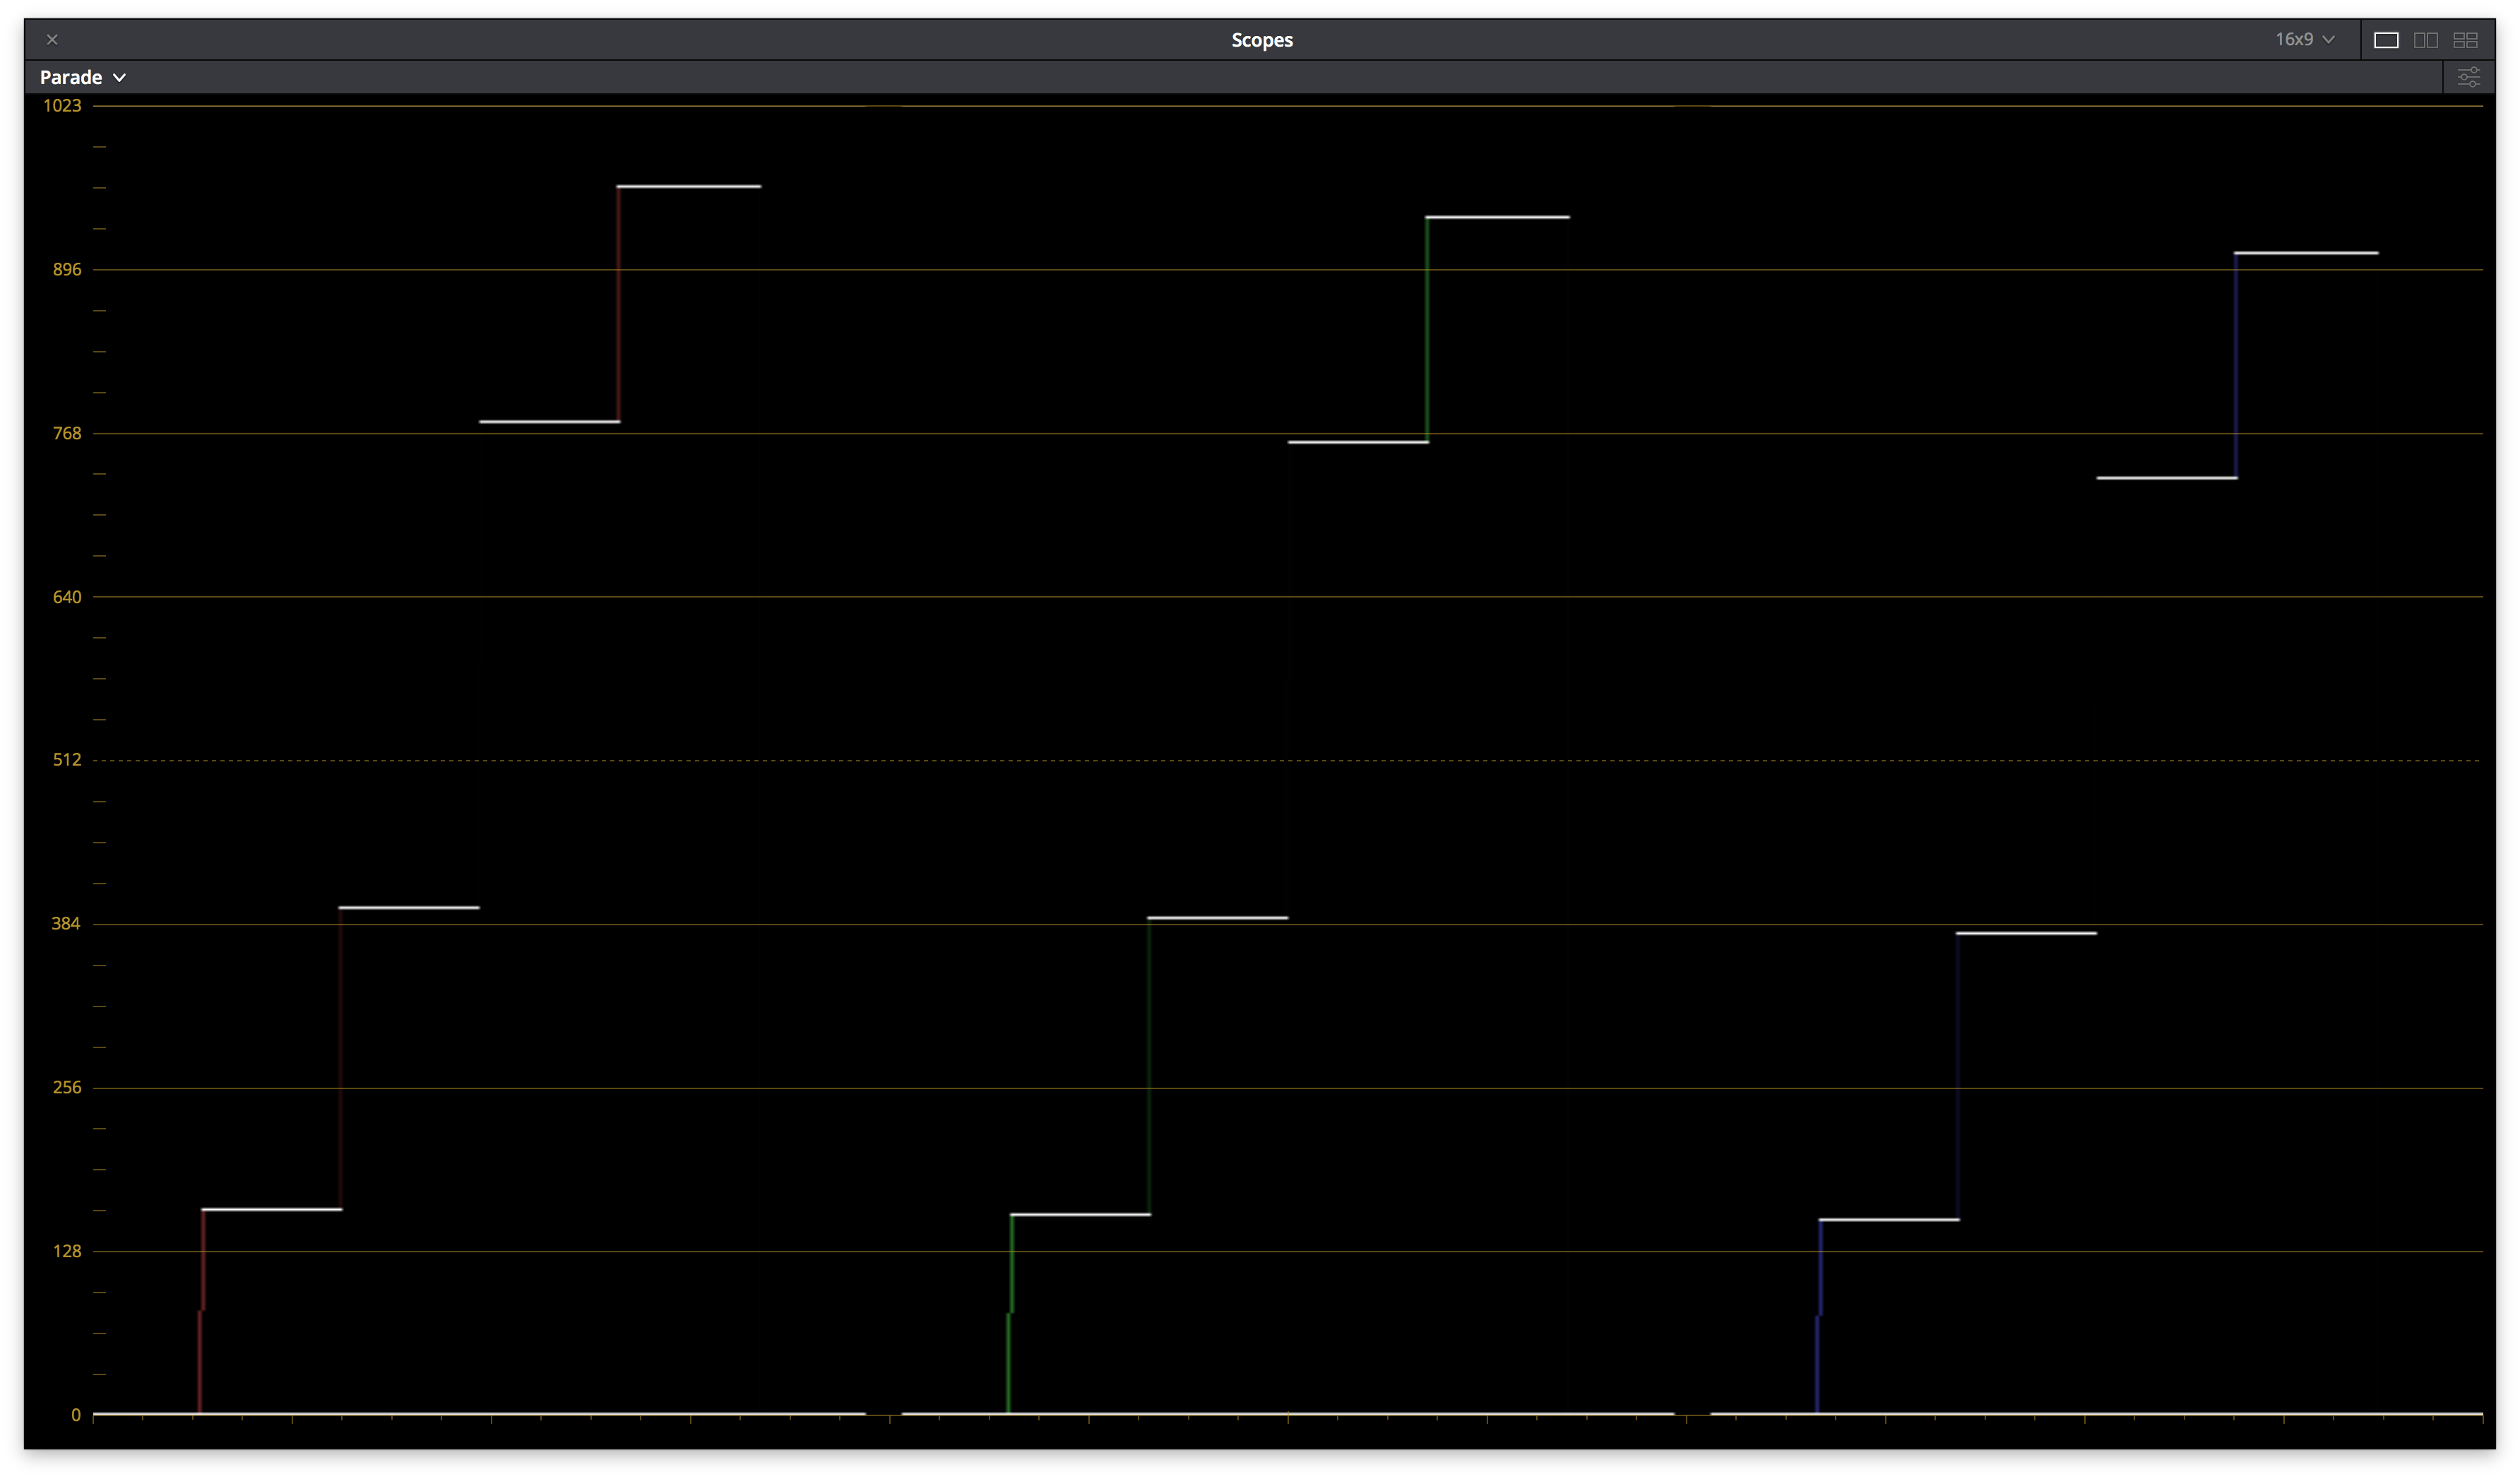
\includegraphics[width=\textwidth]{images/rec709_d60sim/rec709_d60sim_parade}
            \caption[Parade]%
            {{\small Parade}}    
            \label{fig:parade-rec709_d60sim}
        \end{subfigure}
        \quad
        \begin{subfigure}[b]{0.475\textwidth}   
            \centering 
            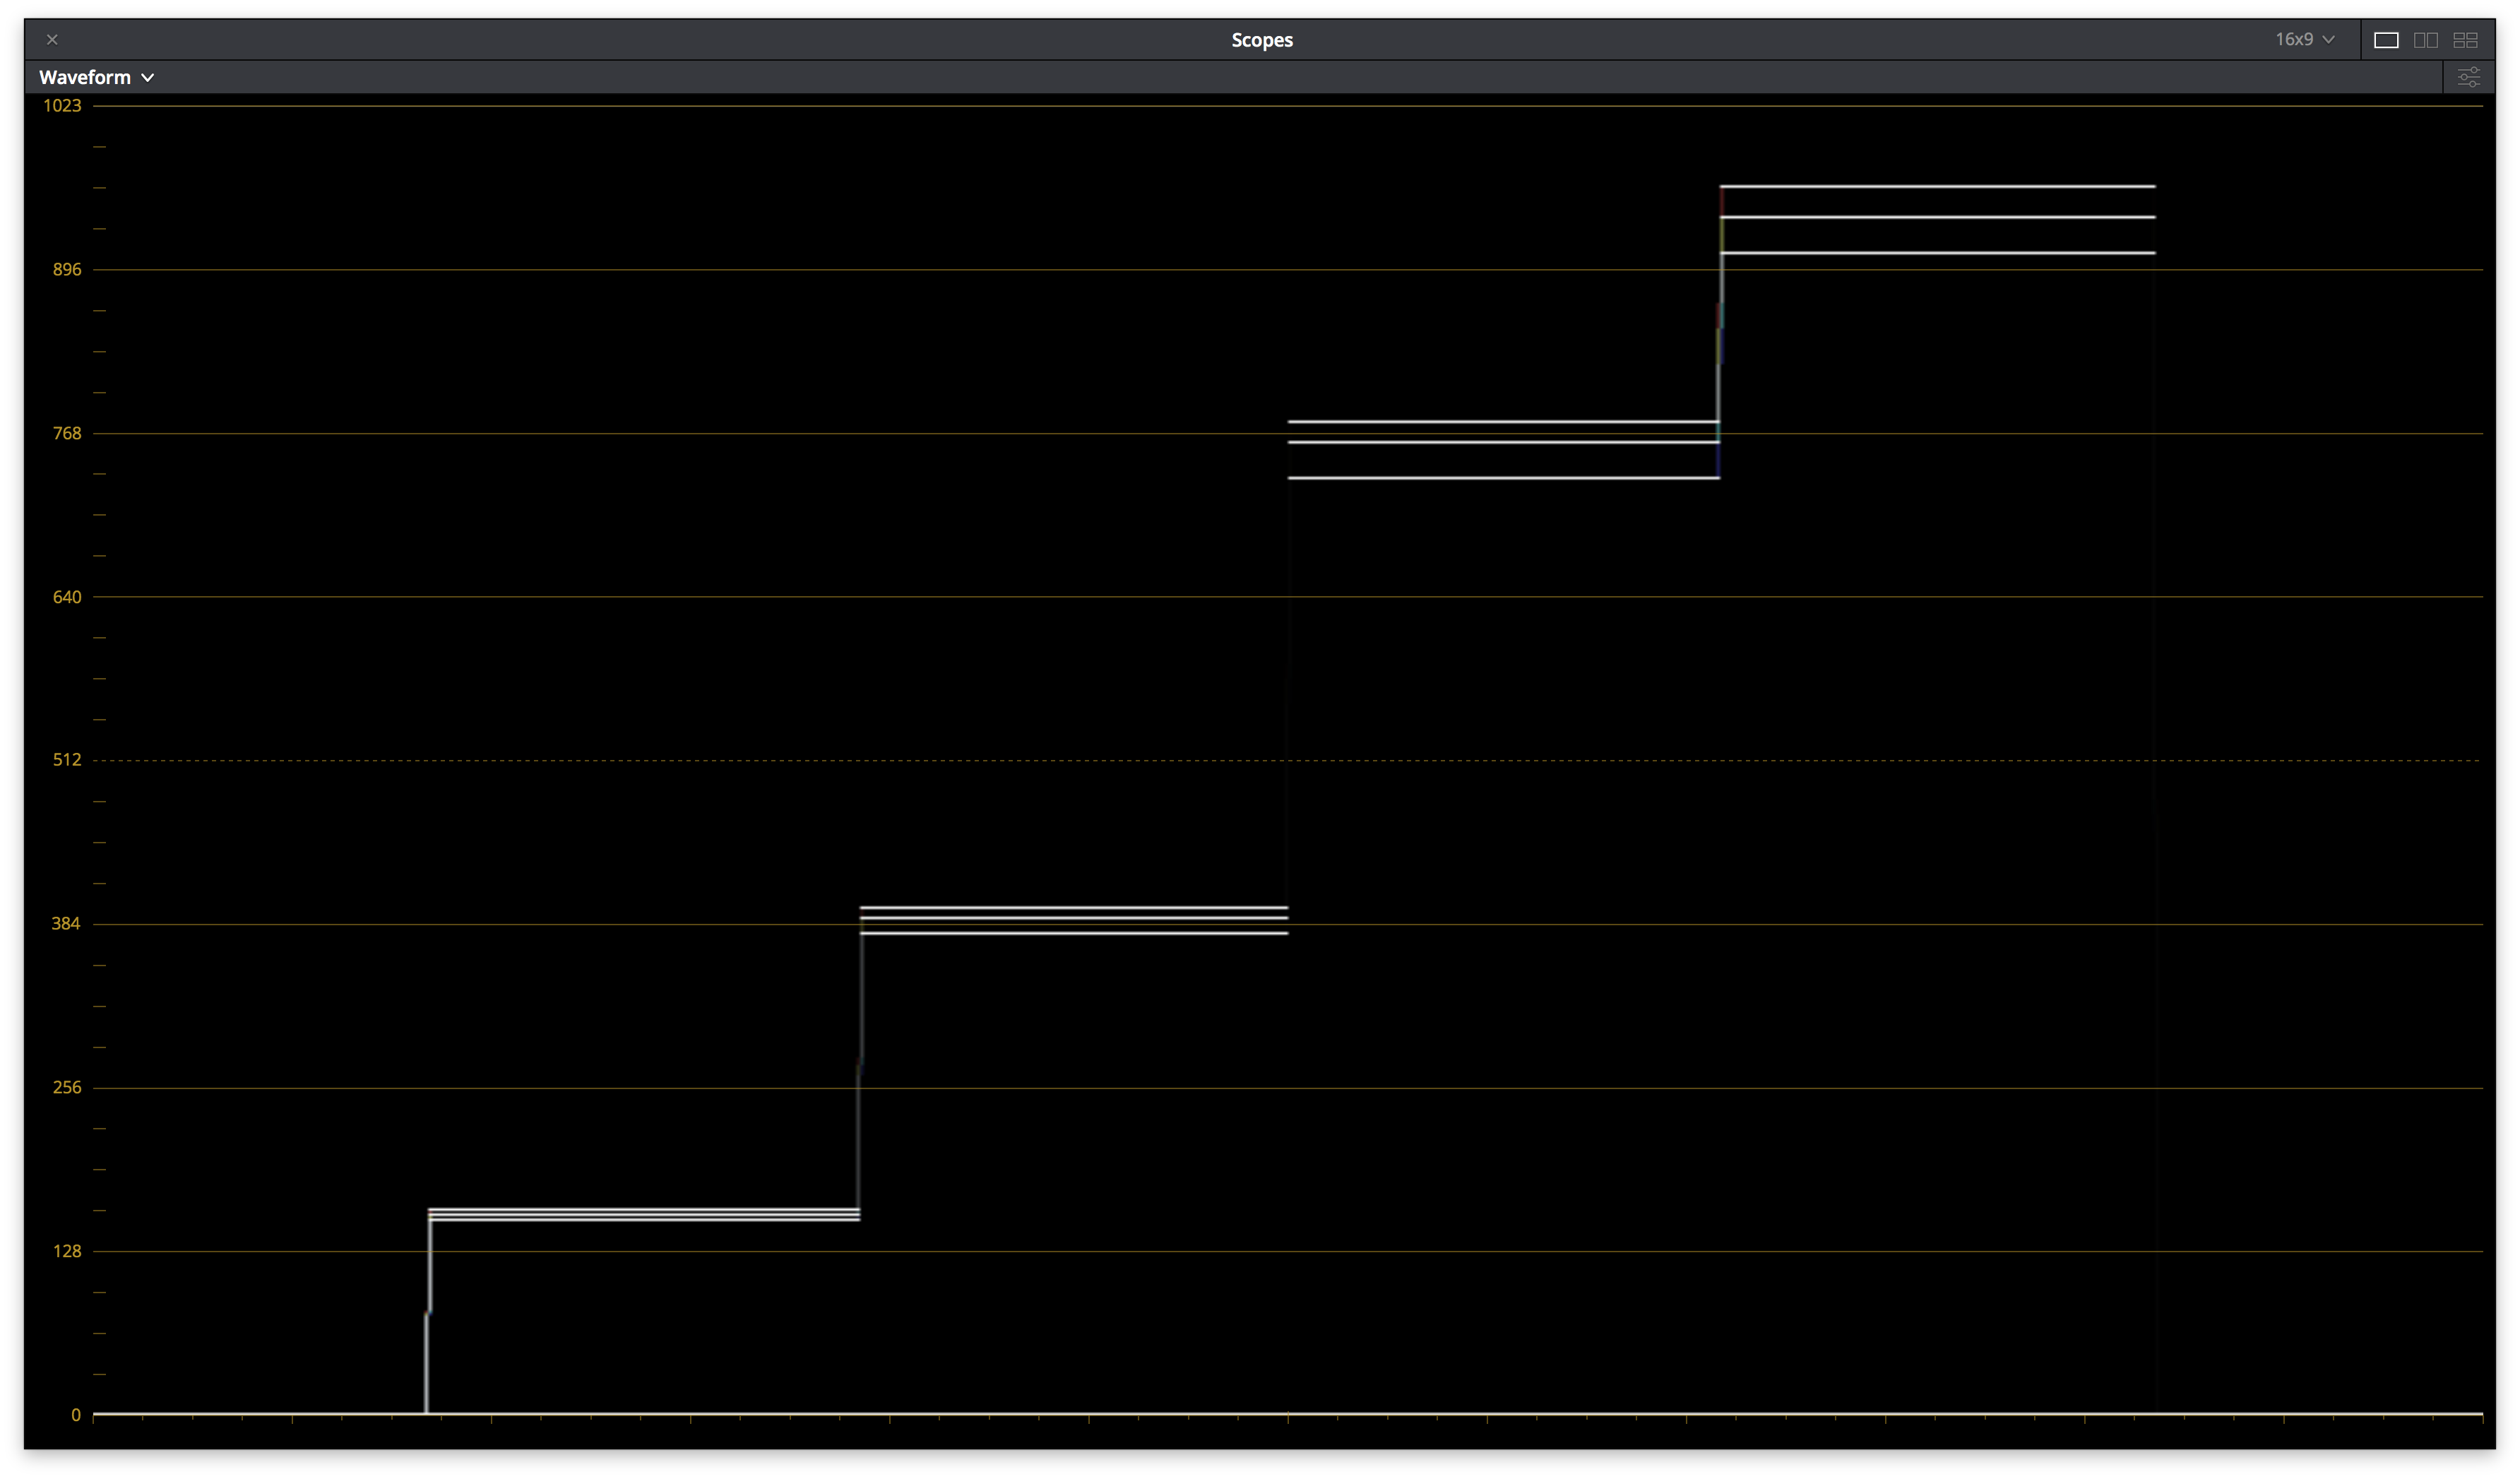
\includegraphics[width=\textwidth]{images/rec709_d60sim/rec709_d60sim_waveform}
            \caption[]%
            {{\small Waveform}}    
            \label{fig:wf-rec709_d60sim}
        \end{subfigure}
        \begin{subfigure}[b]{0.475\textwidth}   
            \centering 
            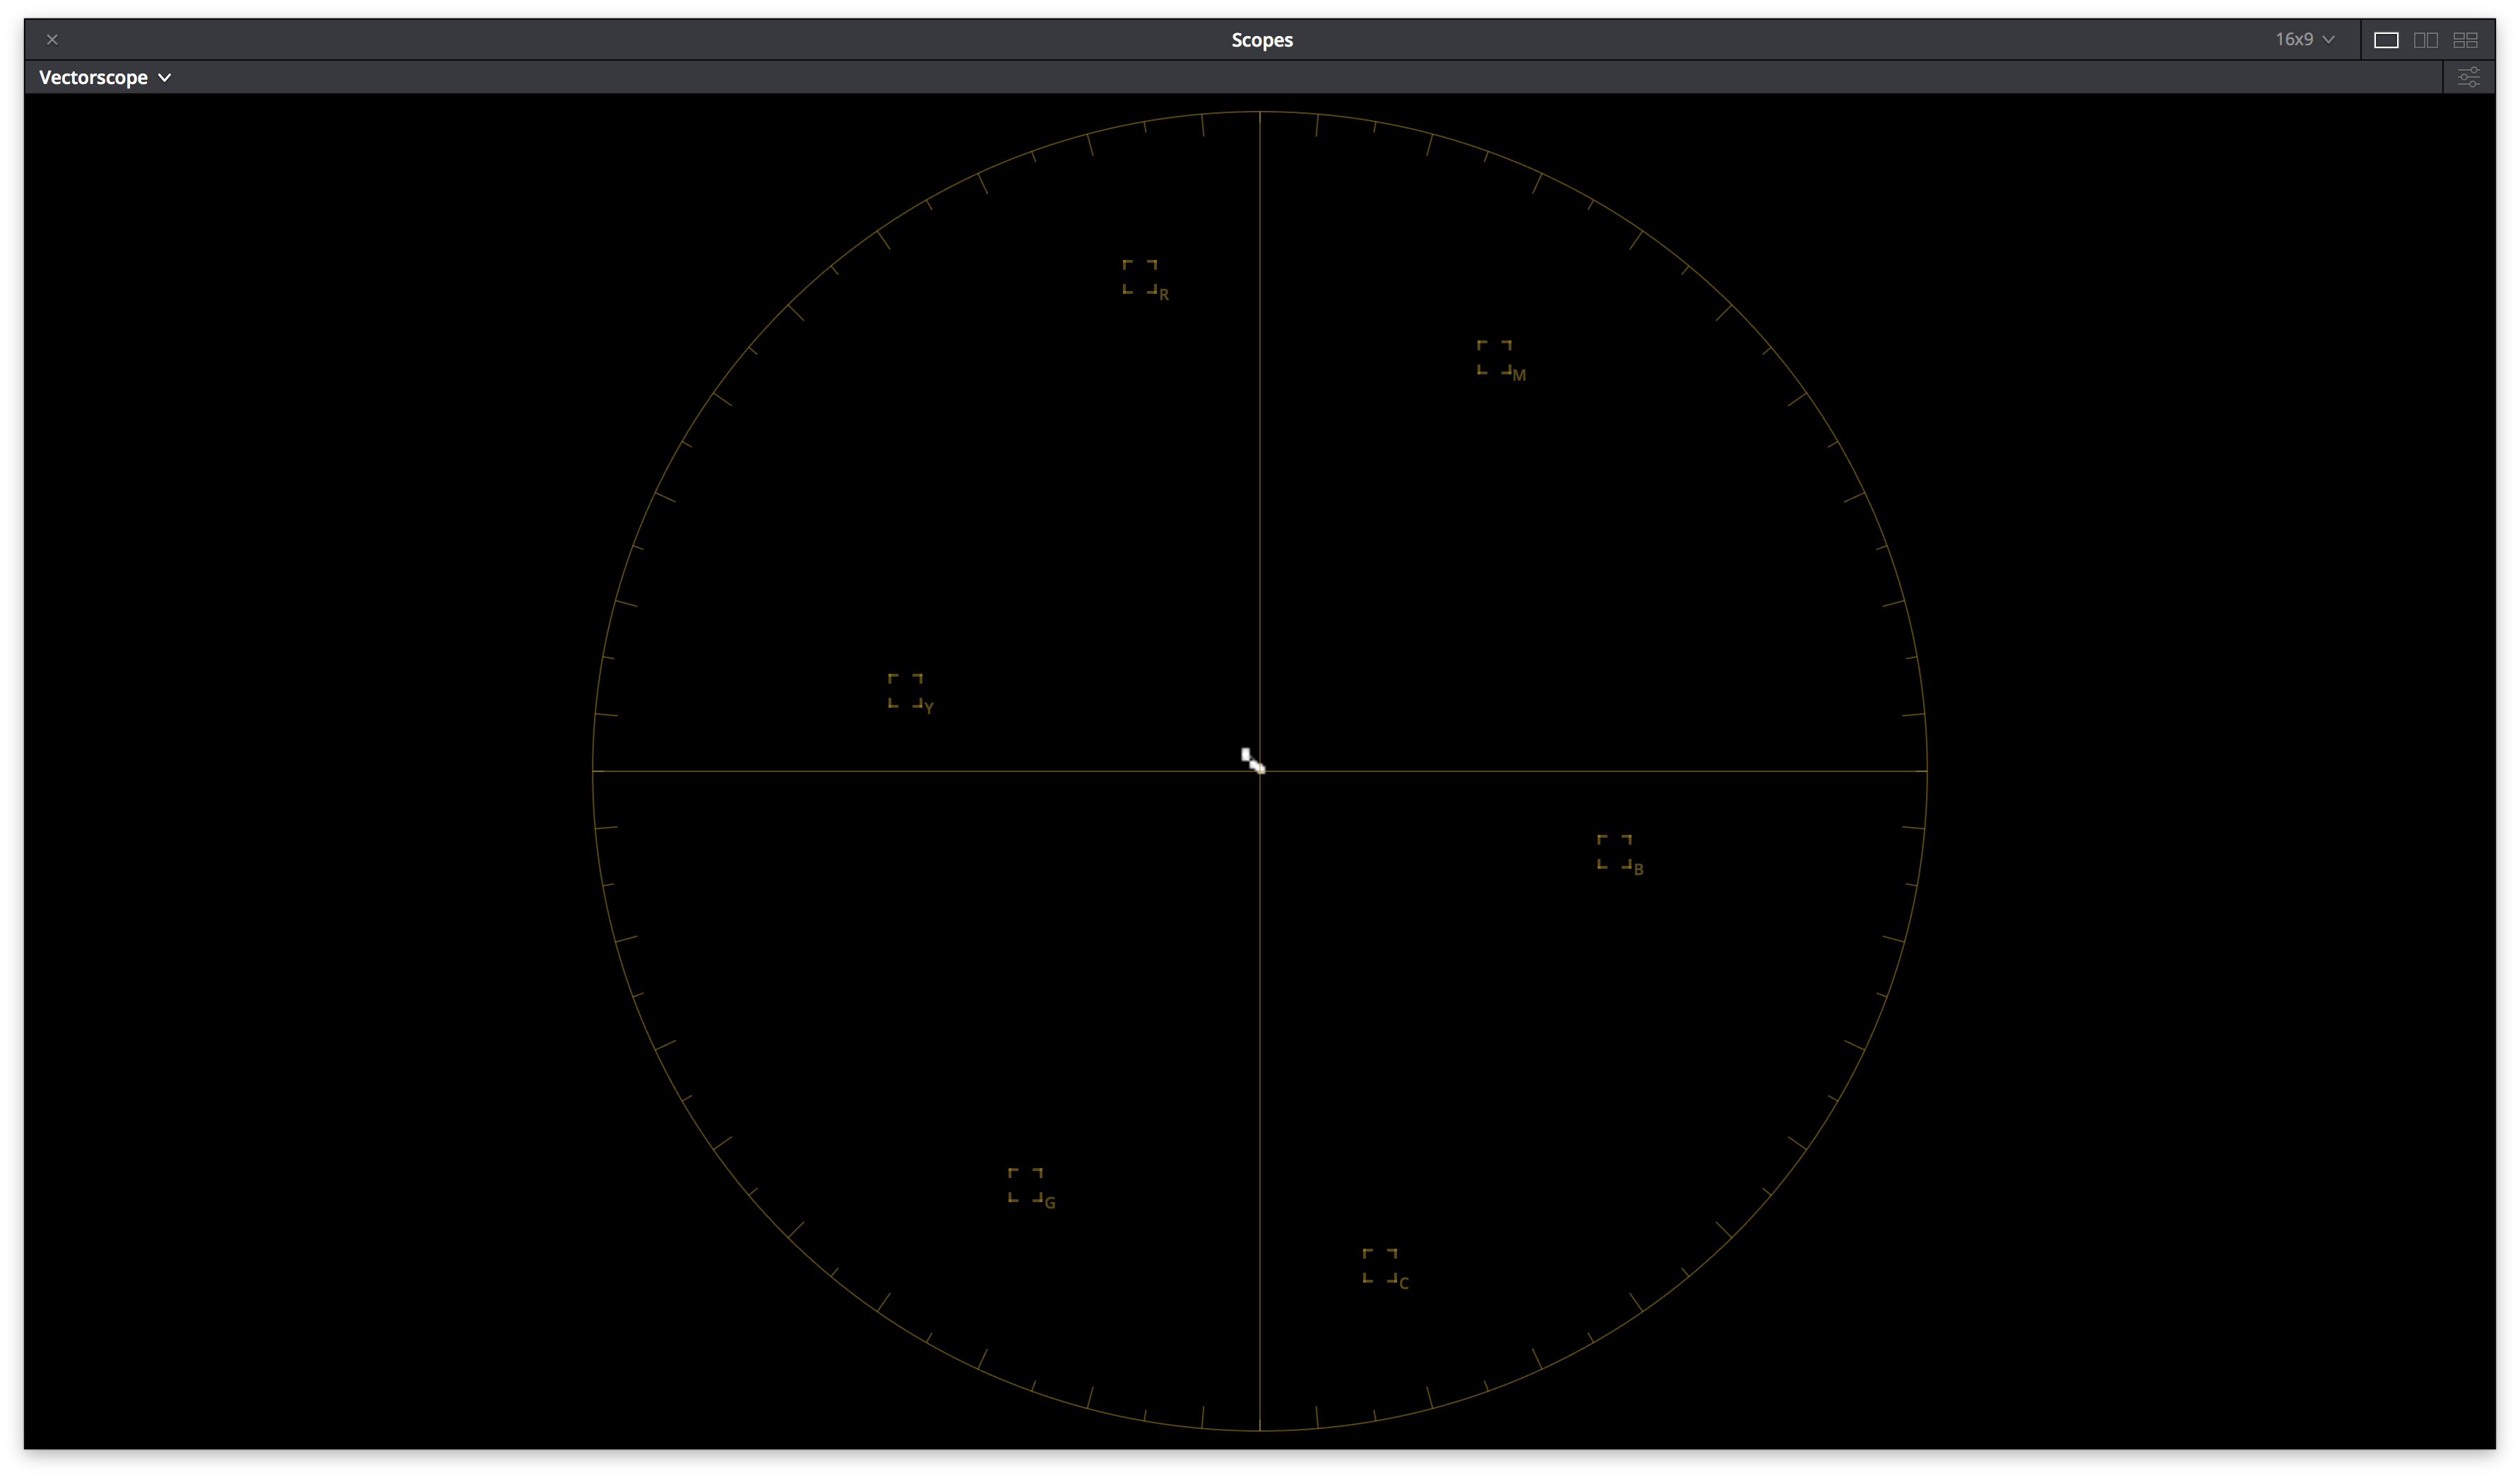
\includegraphics[width=\textwidth]{images/rec709_d60sim/rec709_d60sim_vectorscope}
            \caption[]%
            {{\small vectorscope}}    
            \label{fig:vect-rec709_d60sim}
        \end{subfigure}
        \quad
        \begin{subfigure}[b]{0.475\textwidth}   
            \centering 
            
\includegraphics[width=\textwidth]{images/rec709_d60sim/rec709_d60sim_image}
            \caption[Projector code values as displayed on a D65 calibrated computer monitor]%
            {{\small Projector code values as displayed on a D65 calibrated computer monitor}}    
            \label{fig:cv-rec709_d60sim}
        \end{subfigure}
        \caption[]
        {\small \texttt{\seqsplit{ODT.Academy.Rec709\_100nits\_dim.a1.0.3}} Scope Screenshots} 
        \label{fig:screenshots-rec709_d60sim}
    \end{figure*}


\subsection{Test Values}
\label{subsec:testValues-rec709d60sim}

Table \ref{tab:bestODT-rec709d60sim} contains test values can be used to confirm the proper monitor setup and ODT combination.  Each of the 9 ACES RGB input values should yield the RGB noted display RGB code values (normalized 0-1, full range) when processed through the \texttt{\seqsplit{ODT.Academy.Rec709\_D60sim\_100nits\_dim.a1.0.3}}. When driving a properly setup display with the noted display RGB code values, the light from the display should measure with the noted CIE xyY colorimetry.  

If the display RGB code values do not match those in the table when using the corresponding input ACES RGB code values, it is likely the wrong ODT is being used.  If the proper display RGB code values are being produced by the ODT, but he measured display colorimetry doesn't match the display xyY code values noted, it is likely the display setup is incorrect.

\begin{table}[ht!]
    \centering
    \begin{tabular}{|l|l|l|l|l|l|l|l|l|l|}
        \hline
        \multicolumn{1}{|c|}{\textbf{Patch}} & \multicolumn{3}{c|}{\textbf{ACES RGB}} & \multicolumn{3}{c|}{\textbf{Display RGB}} & \multicolumn{3}{c|}{\textbf{Display xyY}} \\ \hline
        \textbf{N1} & 1.8233 & 1.8233 & 1.8233 & 0.9003 & 0.8812 & 0.8512 & 0.3217 & 0.3377 & 74.2273 \\
        \textbf{N2} & 0.2753 & 0.2753 & 0.2753 & 0.5002 & 0.4896 & 0.4729 & 0.3217 & 0.3377 & 18.1096 \\
        \textbf{N3} & 0.0898 & 0.0898 & 0.0898 & 0.2501 & 0.2448 & 0.2365 & 0.3217 & 0.3377 & 3.4311  \\
        \textbf{R}  & 0.4689 & 0.1193 & 0.0417 & 0.8181 & 0.1449 & 0.1341 & 0.6193 & 0.3312 & 13.8831 \\
        \textbf{G}  & 0.339  & 0.8068 & 0.0936 & 0.2181 & 0.8126 & 0.1111 & 0.3063 & 0.5895 & 44.0469 \\
        \textbf{B}  & 0.2162 & 0.133  & 0.8711 & 0.1642 & 0.1522 & 0.7881 & 0.1587 & 0.0733 & 5.1345  \\
        \textbf{C}  & 0.5187 & 0.9138 & 1.0432 & 0.2268 & 0.8131 & 0.7857 & 0.233  & 0.3397 & 48.1745 \\
        \textbf{M}  & 0.58   & 0.2096 & 0.9086 & 0.8219 & 0.1478 & 0.7874 & 0.3322 & 0.1655 & 18.078  \\
        \textbf{Y}  & 0.8237 & 0.9378 & 0.0855 & 0.8289 & 0.8122 & 0.0999 & 0.422  & 0.5004 & 56.9904 \\
        \hline
        \end{tabular}
        \caption[Theatrical On-Set Preview - Test Values]{\texttt{ODT.Academy.Rec709\_D60sim\_100nits\_dim.a1.0.3} Test Values}
        \label{tab:testValues-rec709d60sim}
\end{table}

%%%% Application - Theatrical On-Set Preview (iPad) %%%% 
\clearpage
\section{Theatrical On-Set Preview (iPad)}
\label{sec:ot-app-iPad-d60sim}

\subsection{Summary}
\label{subsec:summary-iPad-d60sim}

Summarize the application in real world terms

\subsection{Best ODT for application}
\label{subsec:bestODT-iPad-d60sim}

\subsection{Notes}
\label{subsec:notes-iPad-d60sim}

\subsection{Test Values}
\label{subsec:testValues-iPad-d60sim}


%%%% Application -- SDR Broadcast Television Mastering %%%% 
\clearpage
\section{Broadcast Television Mastering (Rec.709 SDR Reference Monitor)}
\label{sec:ot-app-rec709}

\subsection{Summary}
\label{subsec:summary-rec709}

Mastering of episodic television shows and other broadcast content often takes place while viewing images on a standard dynamic range (SDR) Rec.709  Reference Monitor. The display is typically configured such that equal red, green, and blue display code values will produce the chromaticity CIE x=0.3127 y=0.3290 (aka D65) on the screen. With the display
configured in this manner, where the intention is to master content for broadcast, it is recommended that the ACES 1.0 ODT with the transformID \texttt{\seqsplit{ODT.Academy.Rec709\_100nits\_dim.a1.0.3}} be used.

\subsection{Display Setup}
\label{subsec:setup-rec709}

\begin{table}[ht!]
    \centering
        \begin{tabular}{|p{1.25in}|p{3in}|}
            \hline
            \textbf{Parameter} & \textbf{Setting} \\ \hline
            Max Luminance & 100 nits \\ \hline
            Display White Point & D65 \\ \hline
            Primaries & Rec.709  \\ \hline
            EOTF & BT.1886 \\ \hline
            Viewing Environment & dim \\ \hline
            Signal & RGB 4:4:4 (Full range or Legal Range) \\ \hline
            Bit Depth & 10 or 12-bit \\ \hline 
    	\end{tabular}
    \caption[SDR Broadcast Television Mastering - Display Setup]{\small Rec.709 Display Setup} 
    \label{tab:setup-rec709}
\end{table}

\subsection{Best ODT for application} 
\label{subsec:bestODT-rec709}

\begin{table}[ht!]
    \centering
    \begin{tabular}{|p{1.6in}|p{3.1in}|}
        \hline
        \textbf{Simple Name} & \textbf{TransformID} \\ \hline
        ACES 1.0 Output - Rec.709 & \texttt{\seqsplit{ODT.Academy.Rec709\_100nits\_dim.a1.0.3}} \\ \hline
    \end{tabular}
    \caption[SDR Broadcast Television Mastering - Best ODT]{\small Broadcast Television Mastering ODT} 
    \label{tab:bestODT-rec709}
\end{table}

\subsection{Notes}
\label{subsec:notes-rec709}

\texttt{\seqsplit{ODT.Academy.Rec709\_100nits\_dim.a1.0.3}} is intended to be used with a broadcast display that configured such that equal red, green, and blue display code values produce a chromaticity CIE x=0.3127 y=0.3290 (aka D65) on the screen and the content is intended to be viewed in a typical home viewing environment. The output transform is configured such that neutral ACES source file values (ACES R=G=B) will produce equal
projector code values. In this application, the resulting content will inter-cut with content produced using other video workflows.  Care should be taken to configure choose the proper output range as the ODT supports both full and legal range.

It's important to note that the image on display screen should be similar in color balance to content produced with other video workflows. The color corrector scopes should reflect this white balance similarity by producing equal red, green and blue display code values for neutral ACES source file values. The scopes may however appear different in range to some video workflows.  In ACES based workflows dynamic range of the source content is maintained by manipulating the content prior to the output transforms.  The shape of the output transform tone scale may be reflected in the display code values being monitored on the color corrector scopes.  This is common with other video workflows where a look-up table (LUT) is used.

    \begin{figure*}[ht!]
        \centering
        \begin{subfigure}[b]{0.475\textwidth}
            \centering
            
\includegraphics[width=\textwidth]{images/aces}
            \caption[Source ACES Image]%
            {{\small ACES Image}}    
            \label{fig:acesSource-rec709}
        \end{subfigure}
        \hfill
        \begin{subfigure}[b]{0.475\textwidth}  
            \centering 
            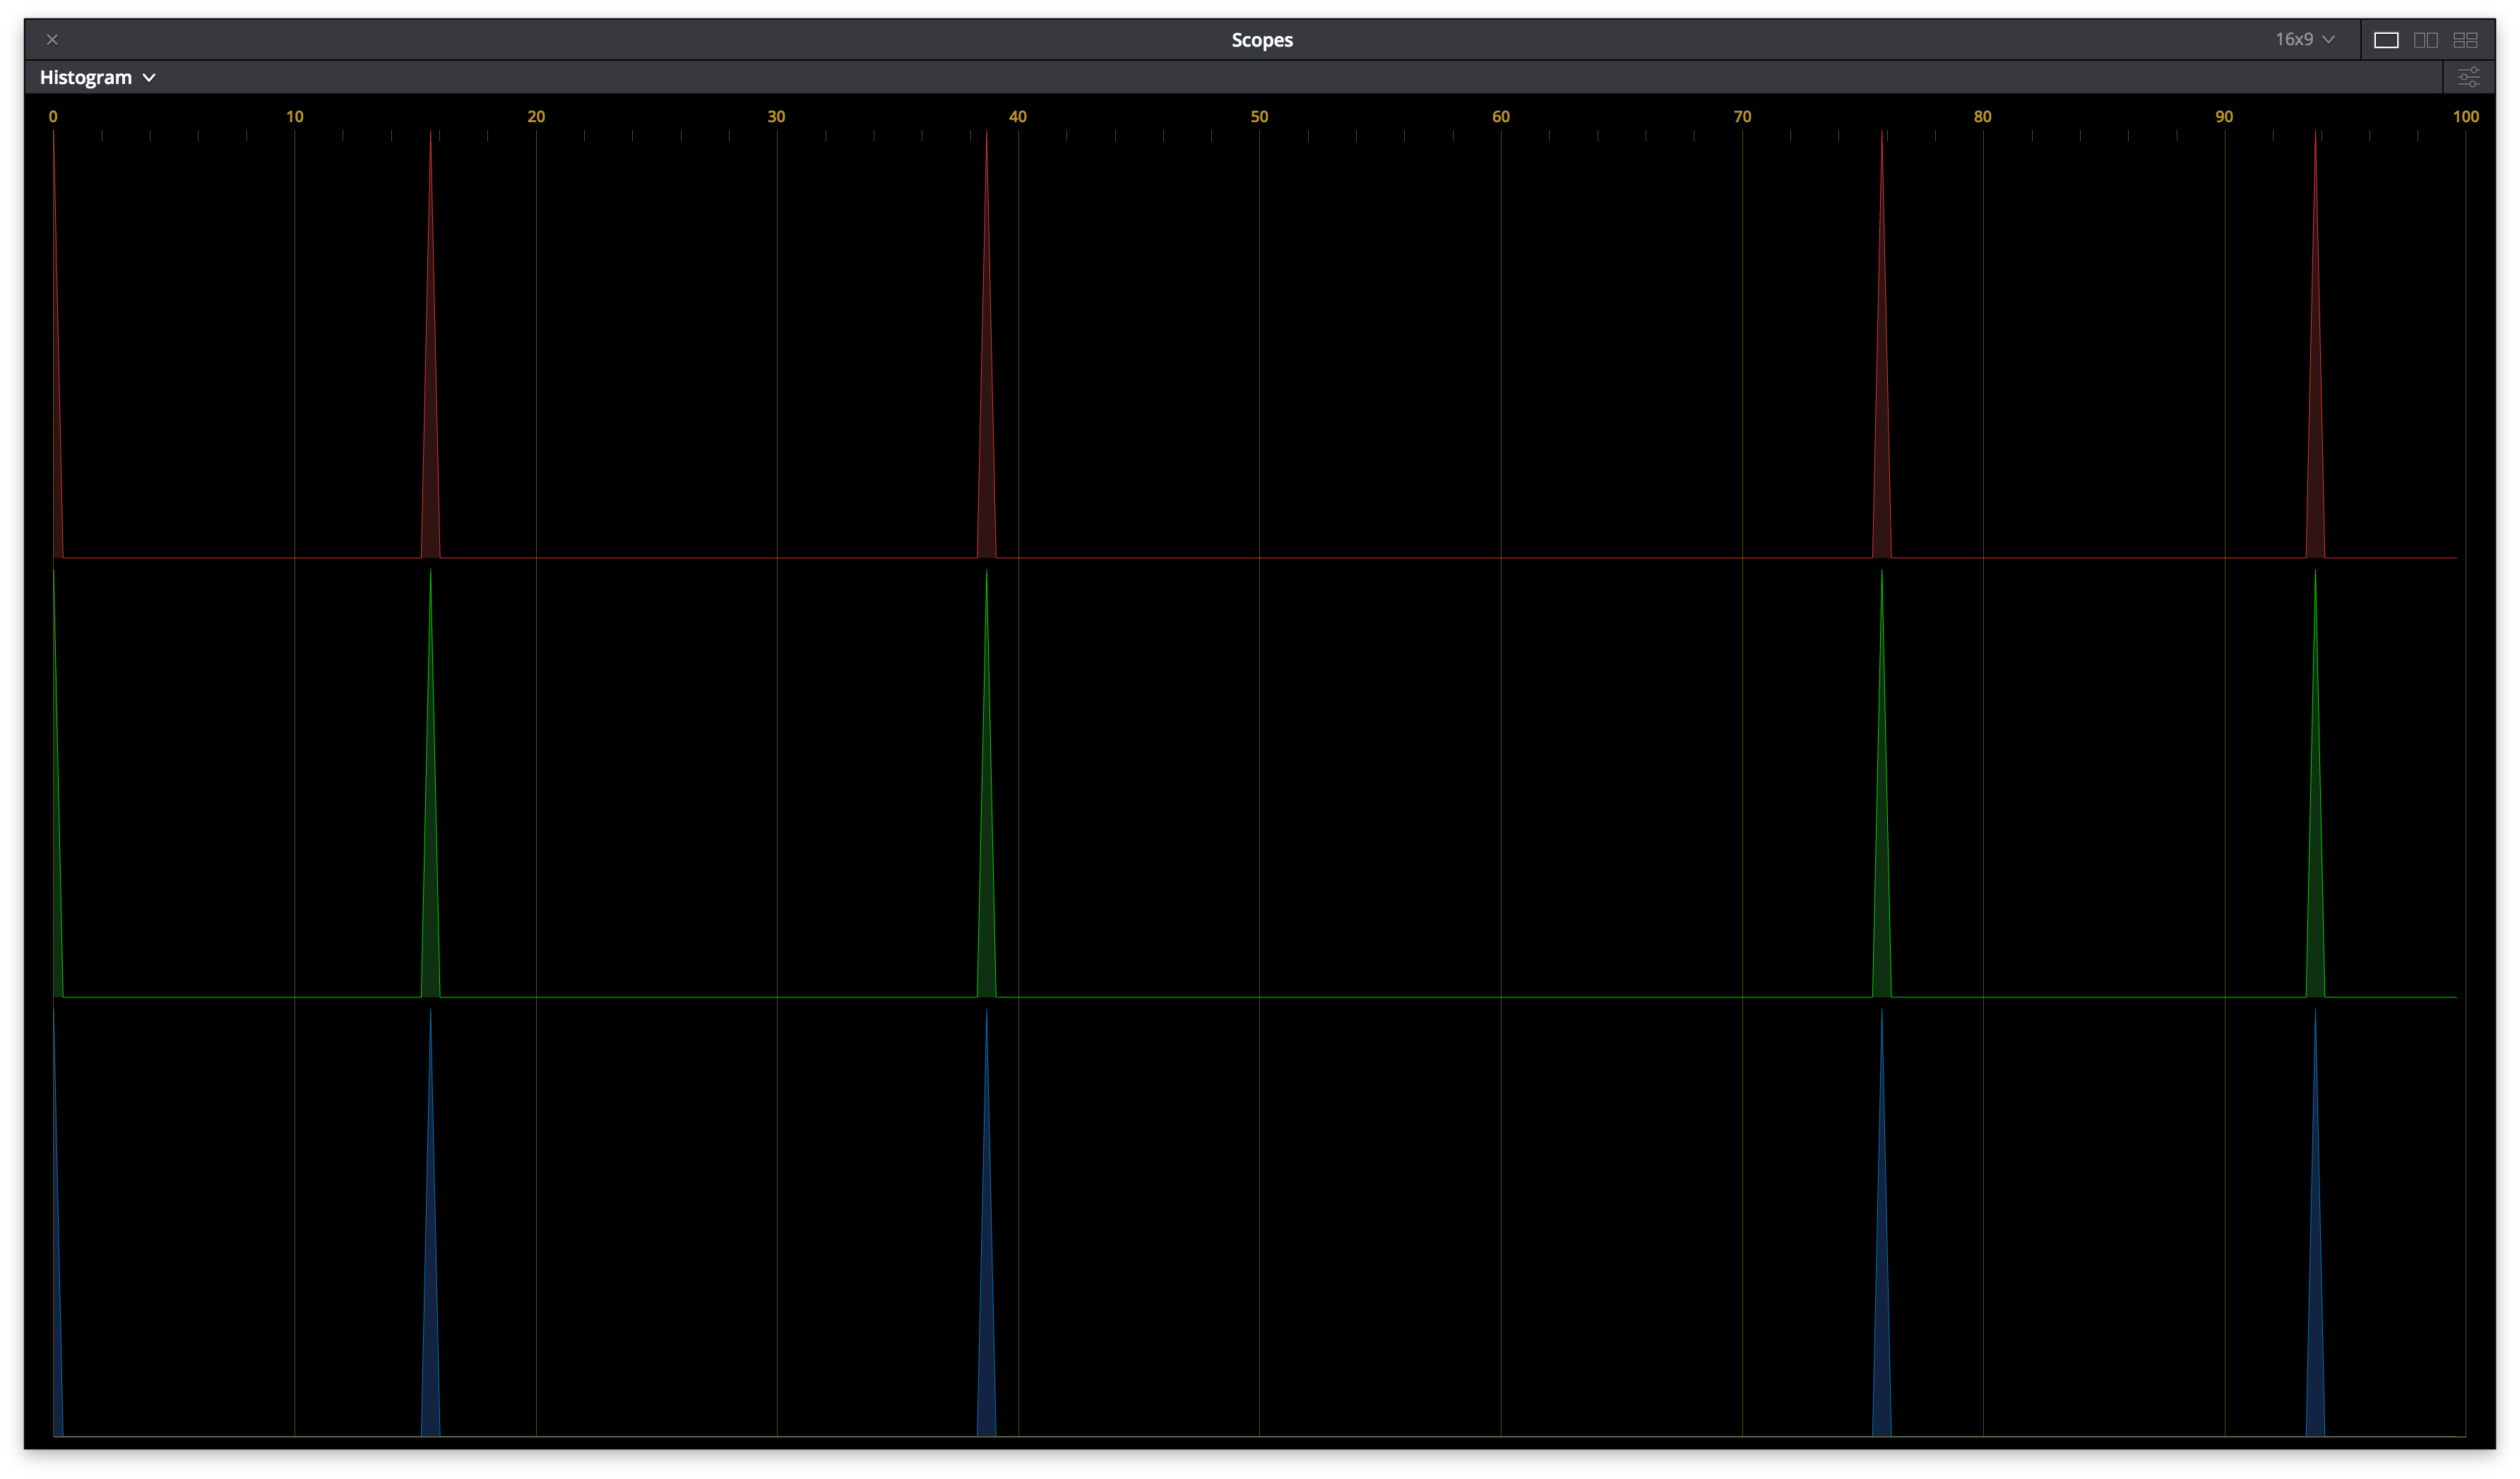
\includegraphics[width=\textwidth]{images/rec709/rec709_histogram}
            \caption[Histogram]%
            {{\small Histogram}}    
            \label{fig:hist-rec709}
        \end{subfigure}
        \vskip\baselineskip
        \begin{subfigure}[b]{0.475\textwidth}   
            \centering 
            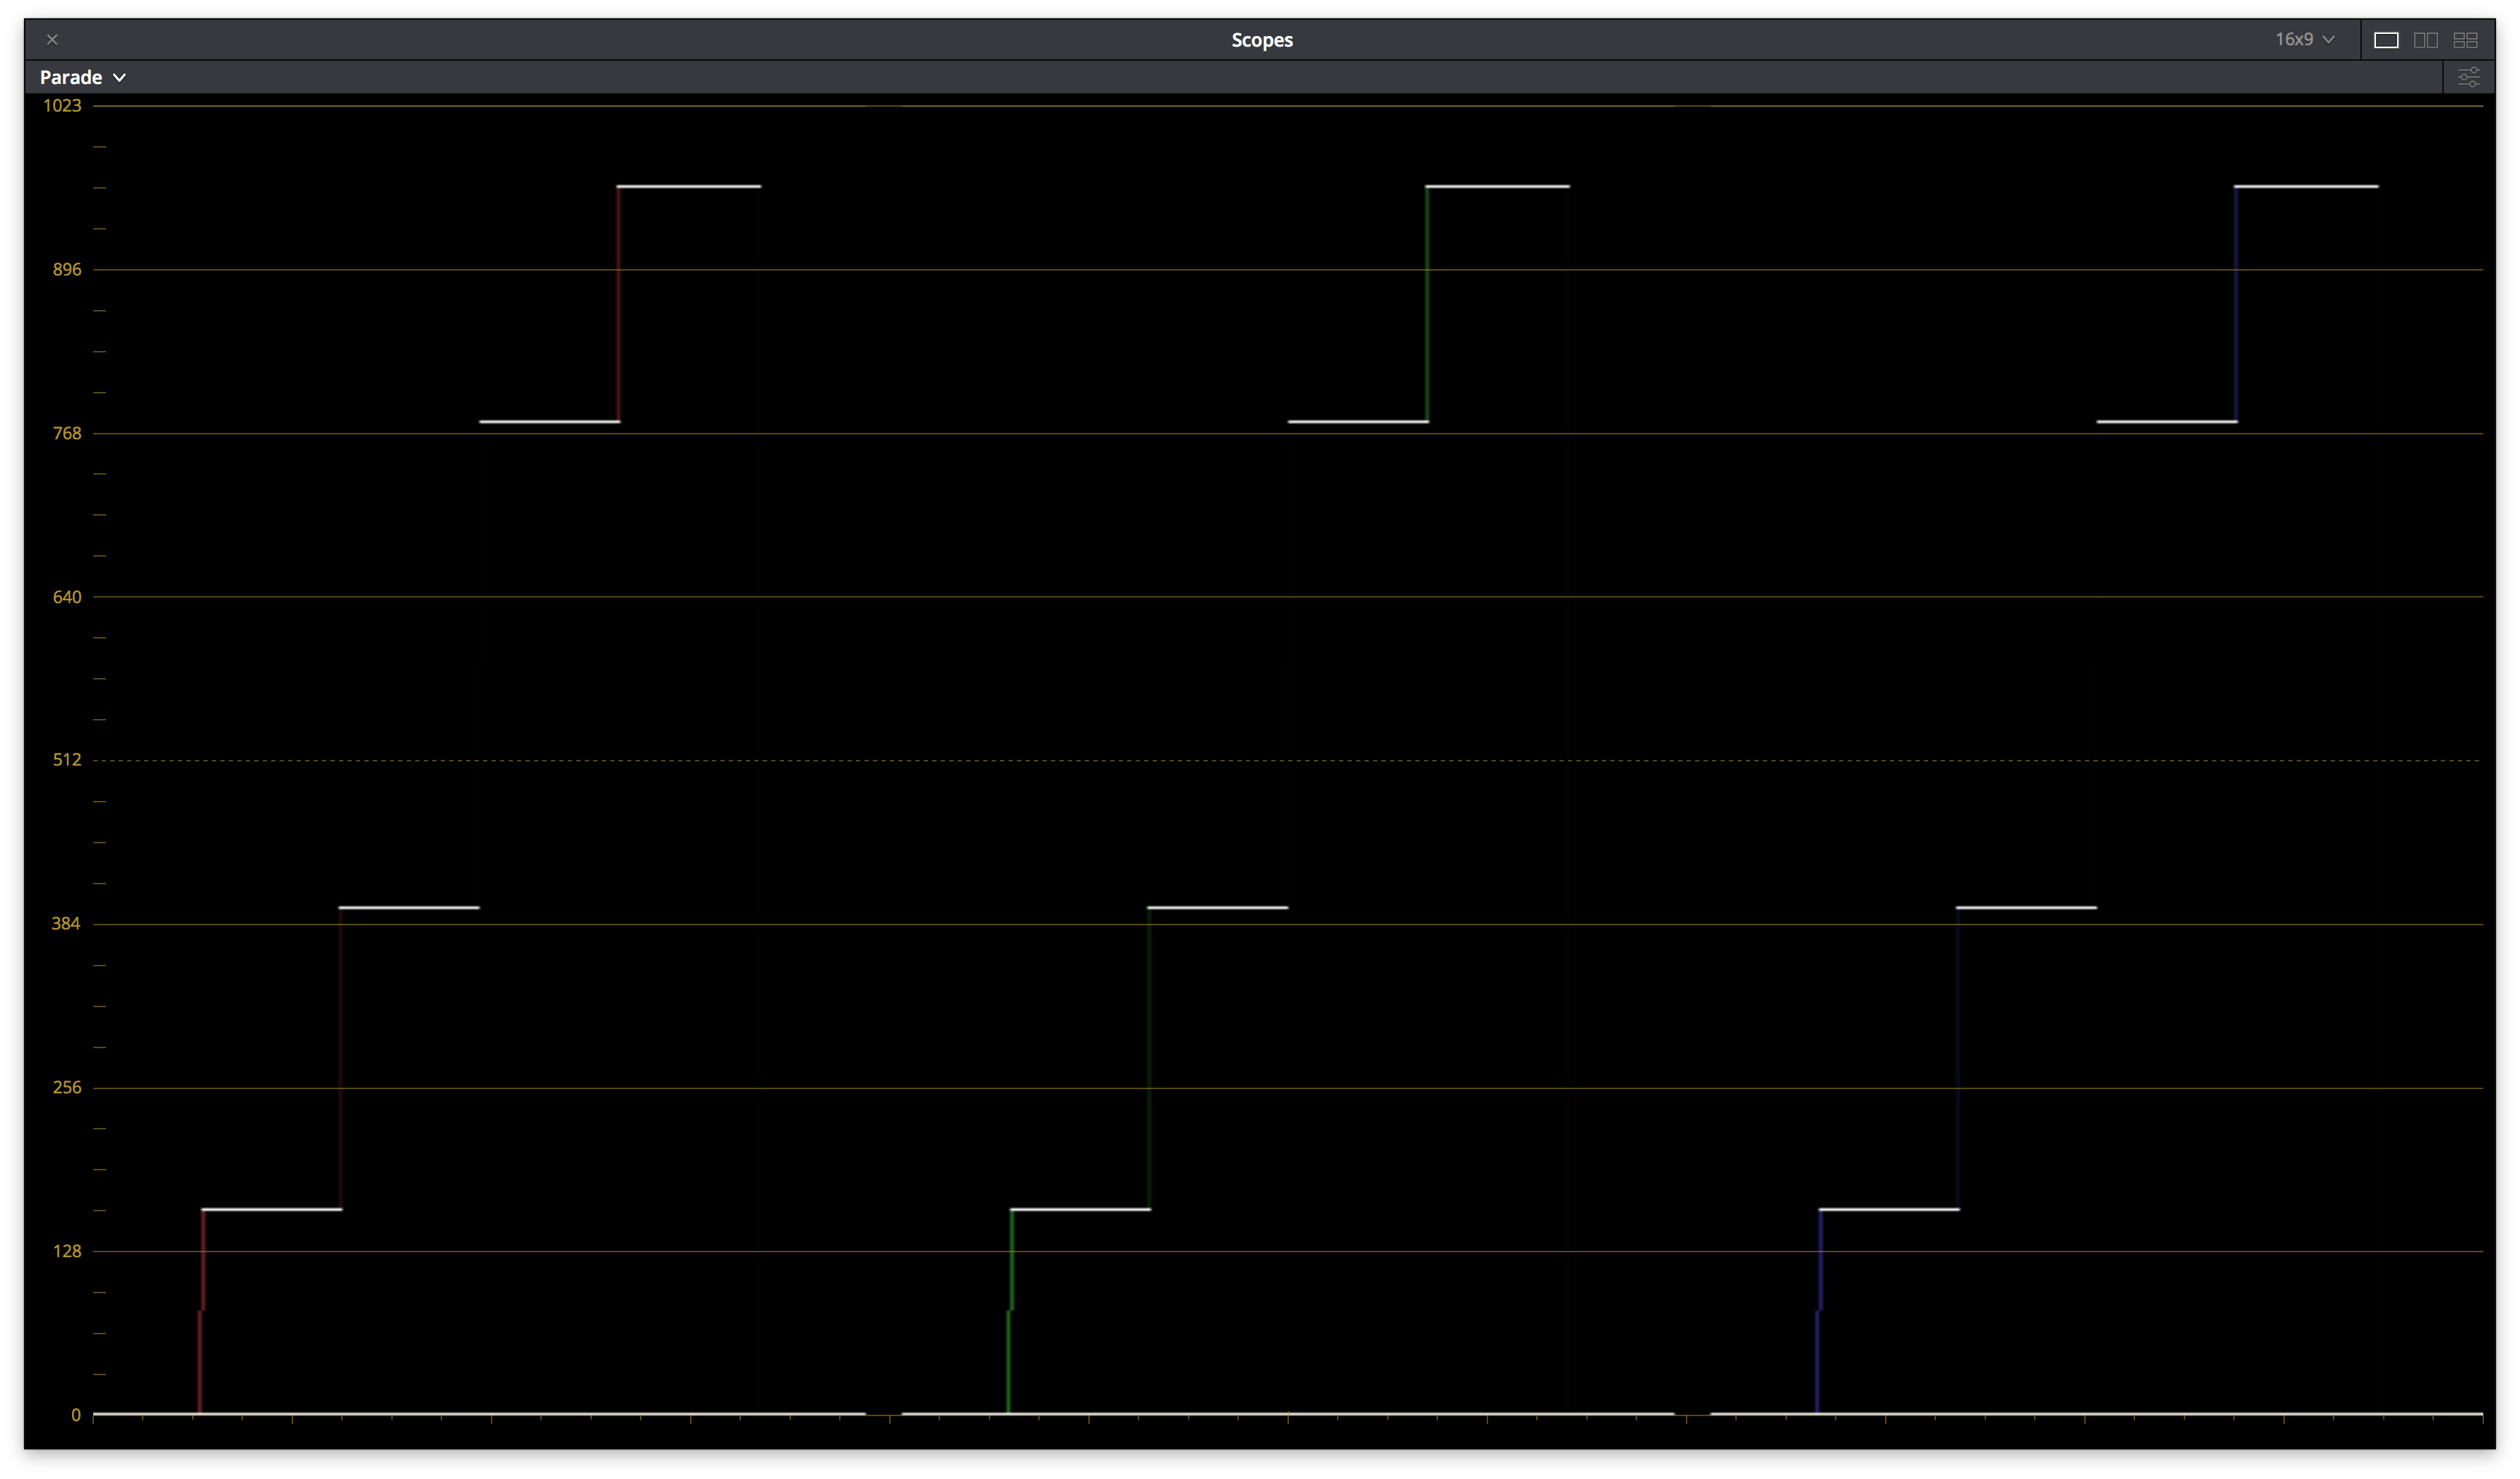
\includegraphics[width=\textwidth]{images/rec709/rec709_parade}
            \caption[Parade]%
            {{\small Parade}}    
            \label{fig:parade-rec709}
        \end{subfigure}
        \quad
        \begin{subfigure}[b]{0.475\textwidth}   
            \centering 
            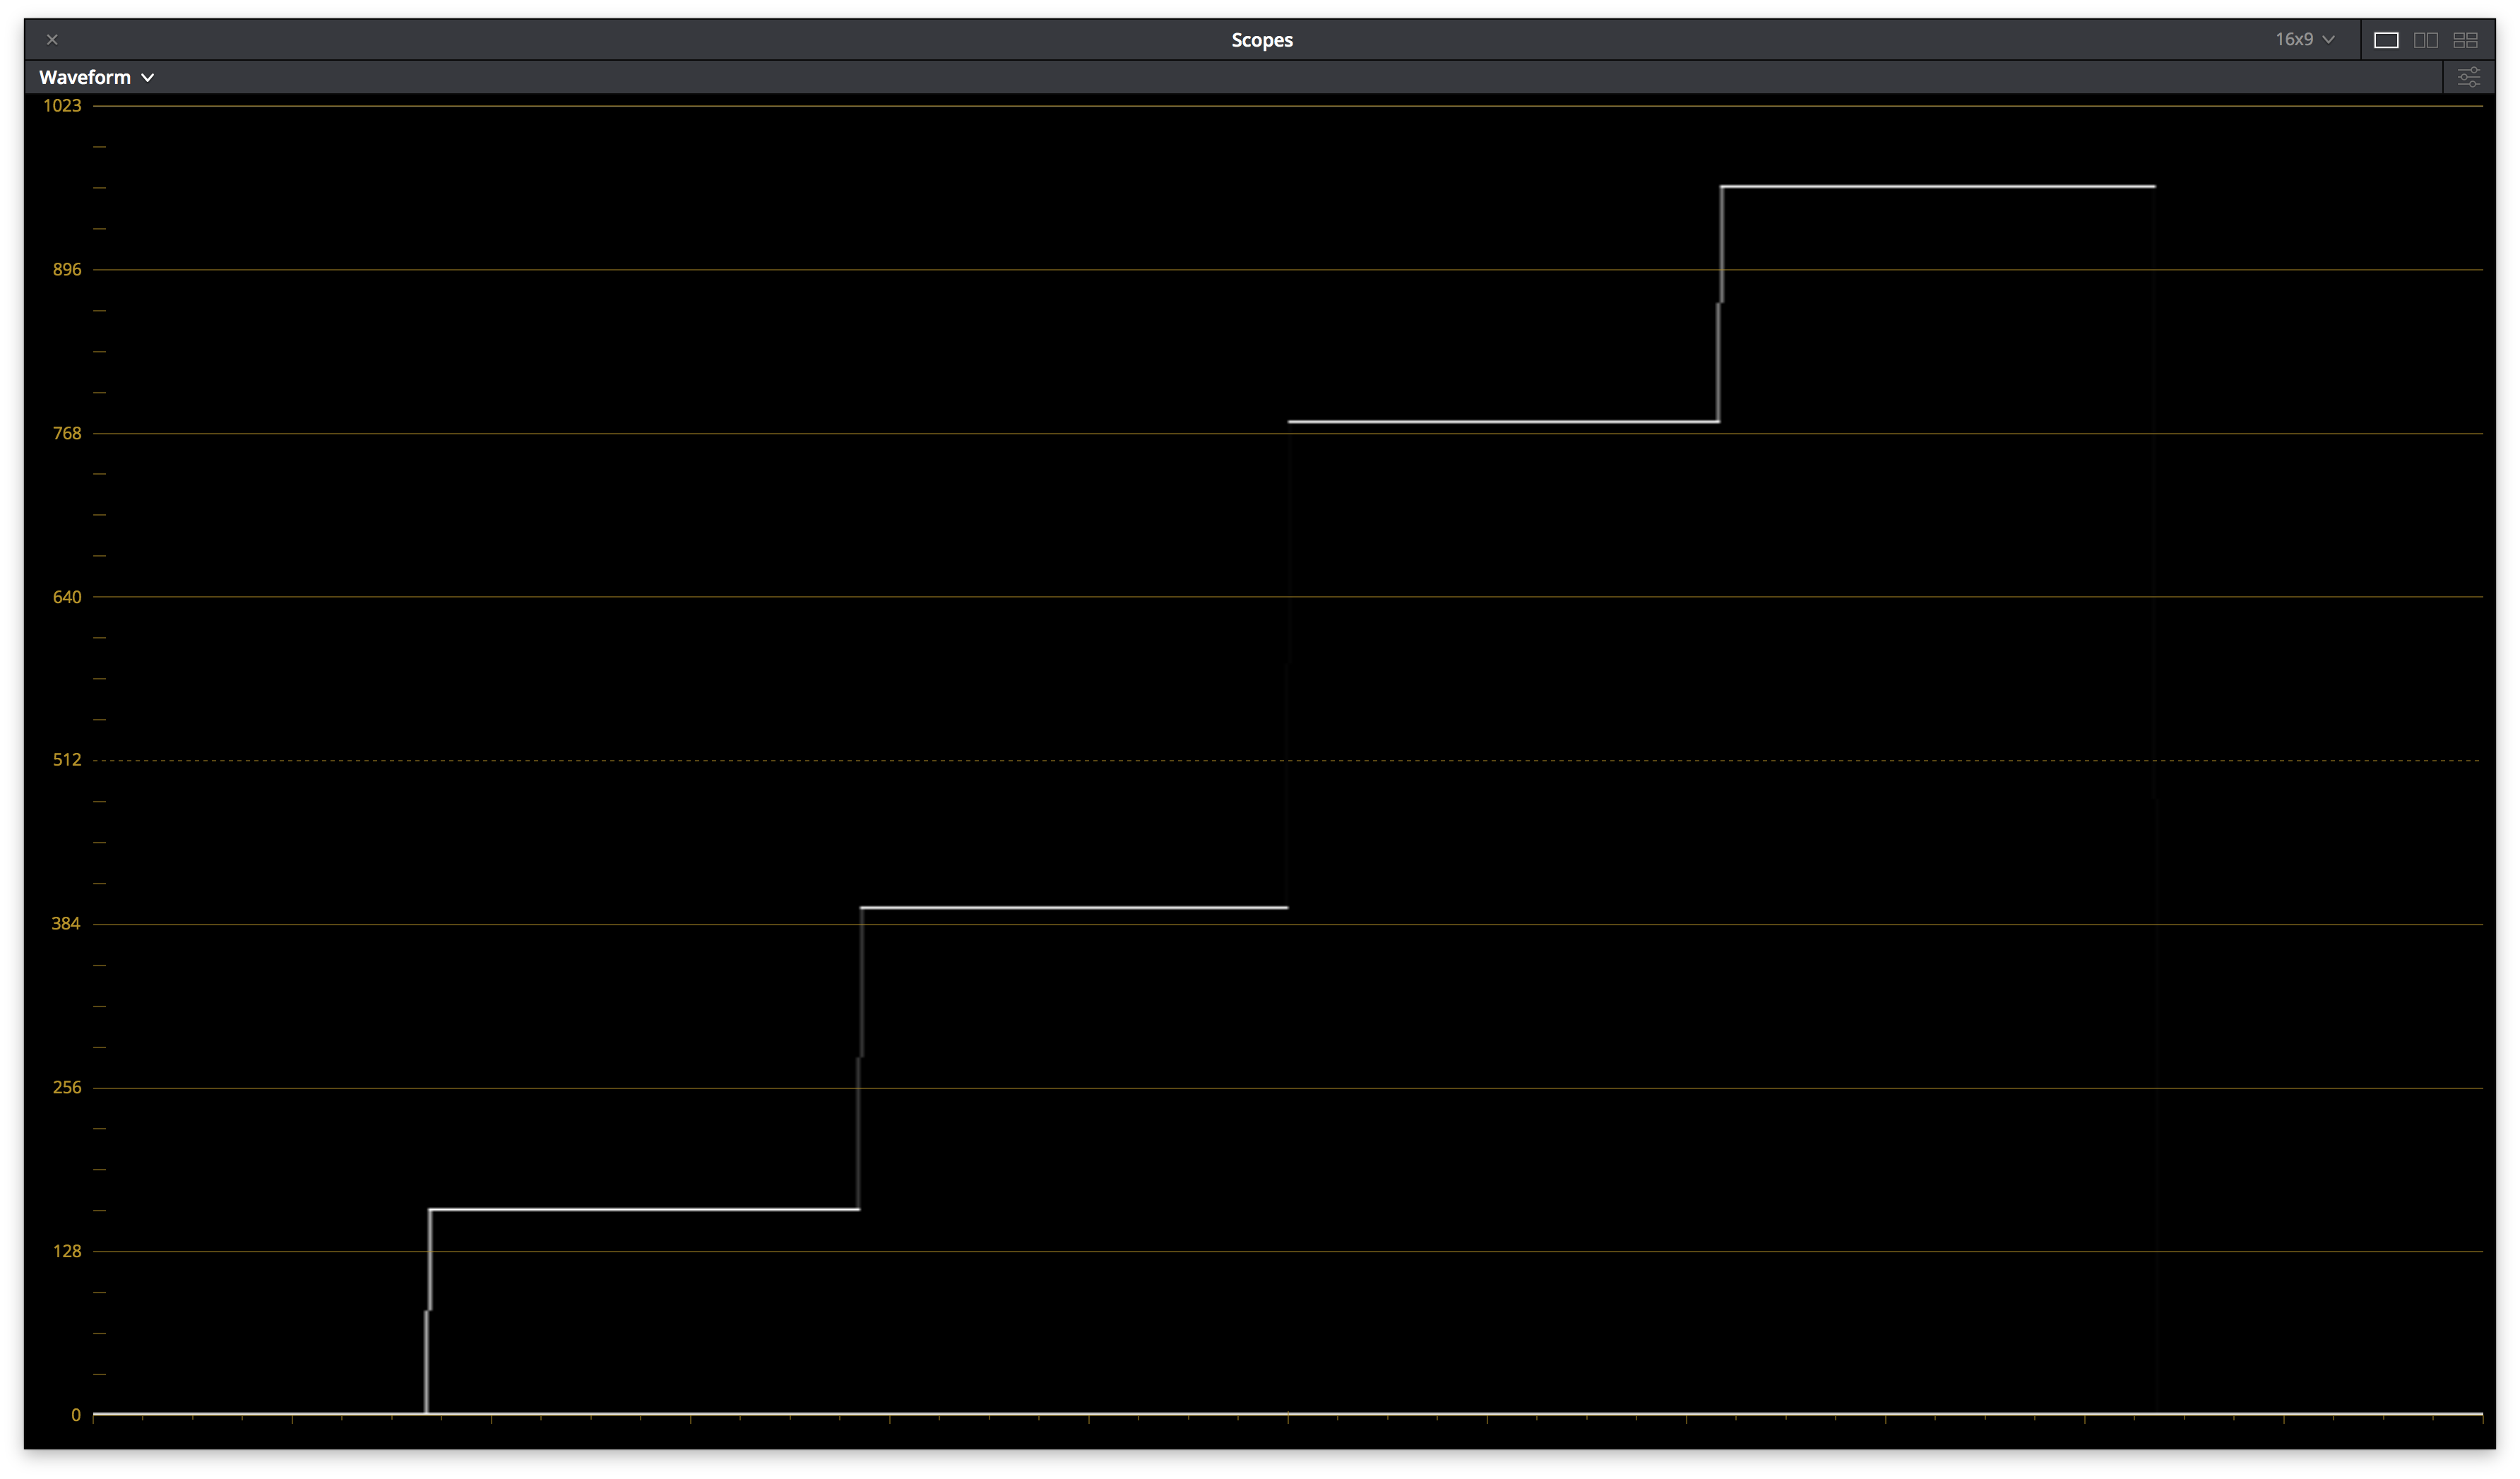
\includegraphics[width=\textwidth]{images/rec709/rec709_waveform}
            \caption[]%
            {{\small Waveform}}    
            \label{fig:wf-rec709}
        \end{subfigure}
        \begin{subfigure}[b]{0.475\textwidth}   
            \centering 
            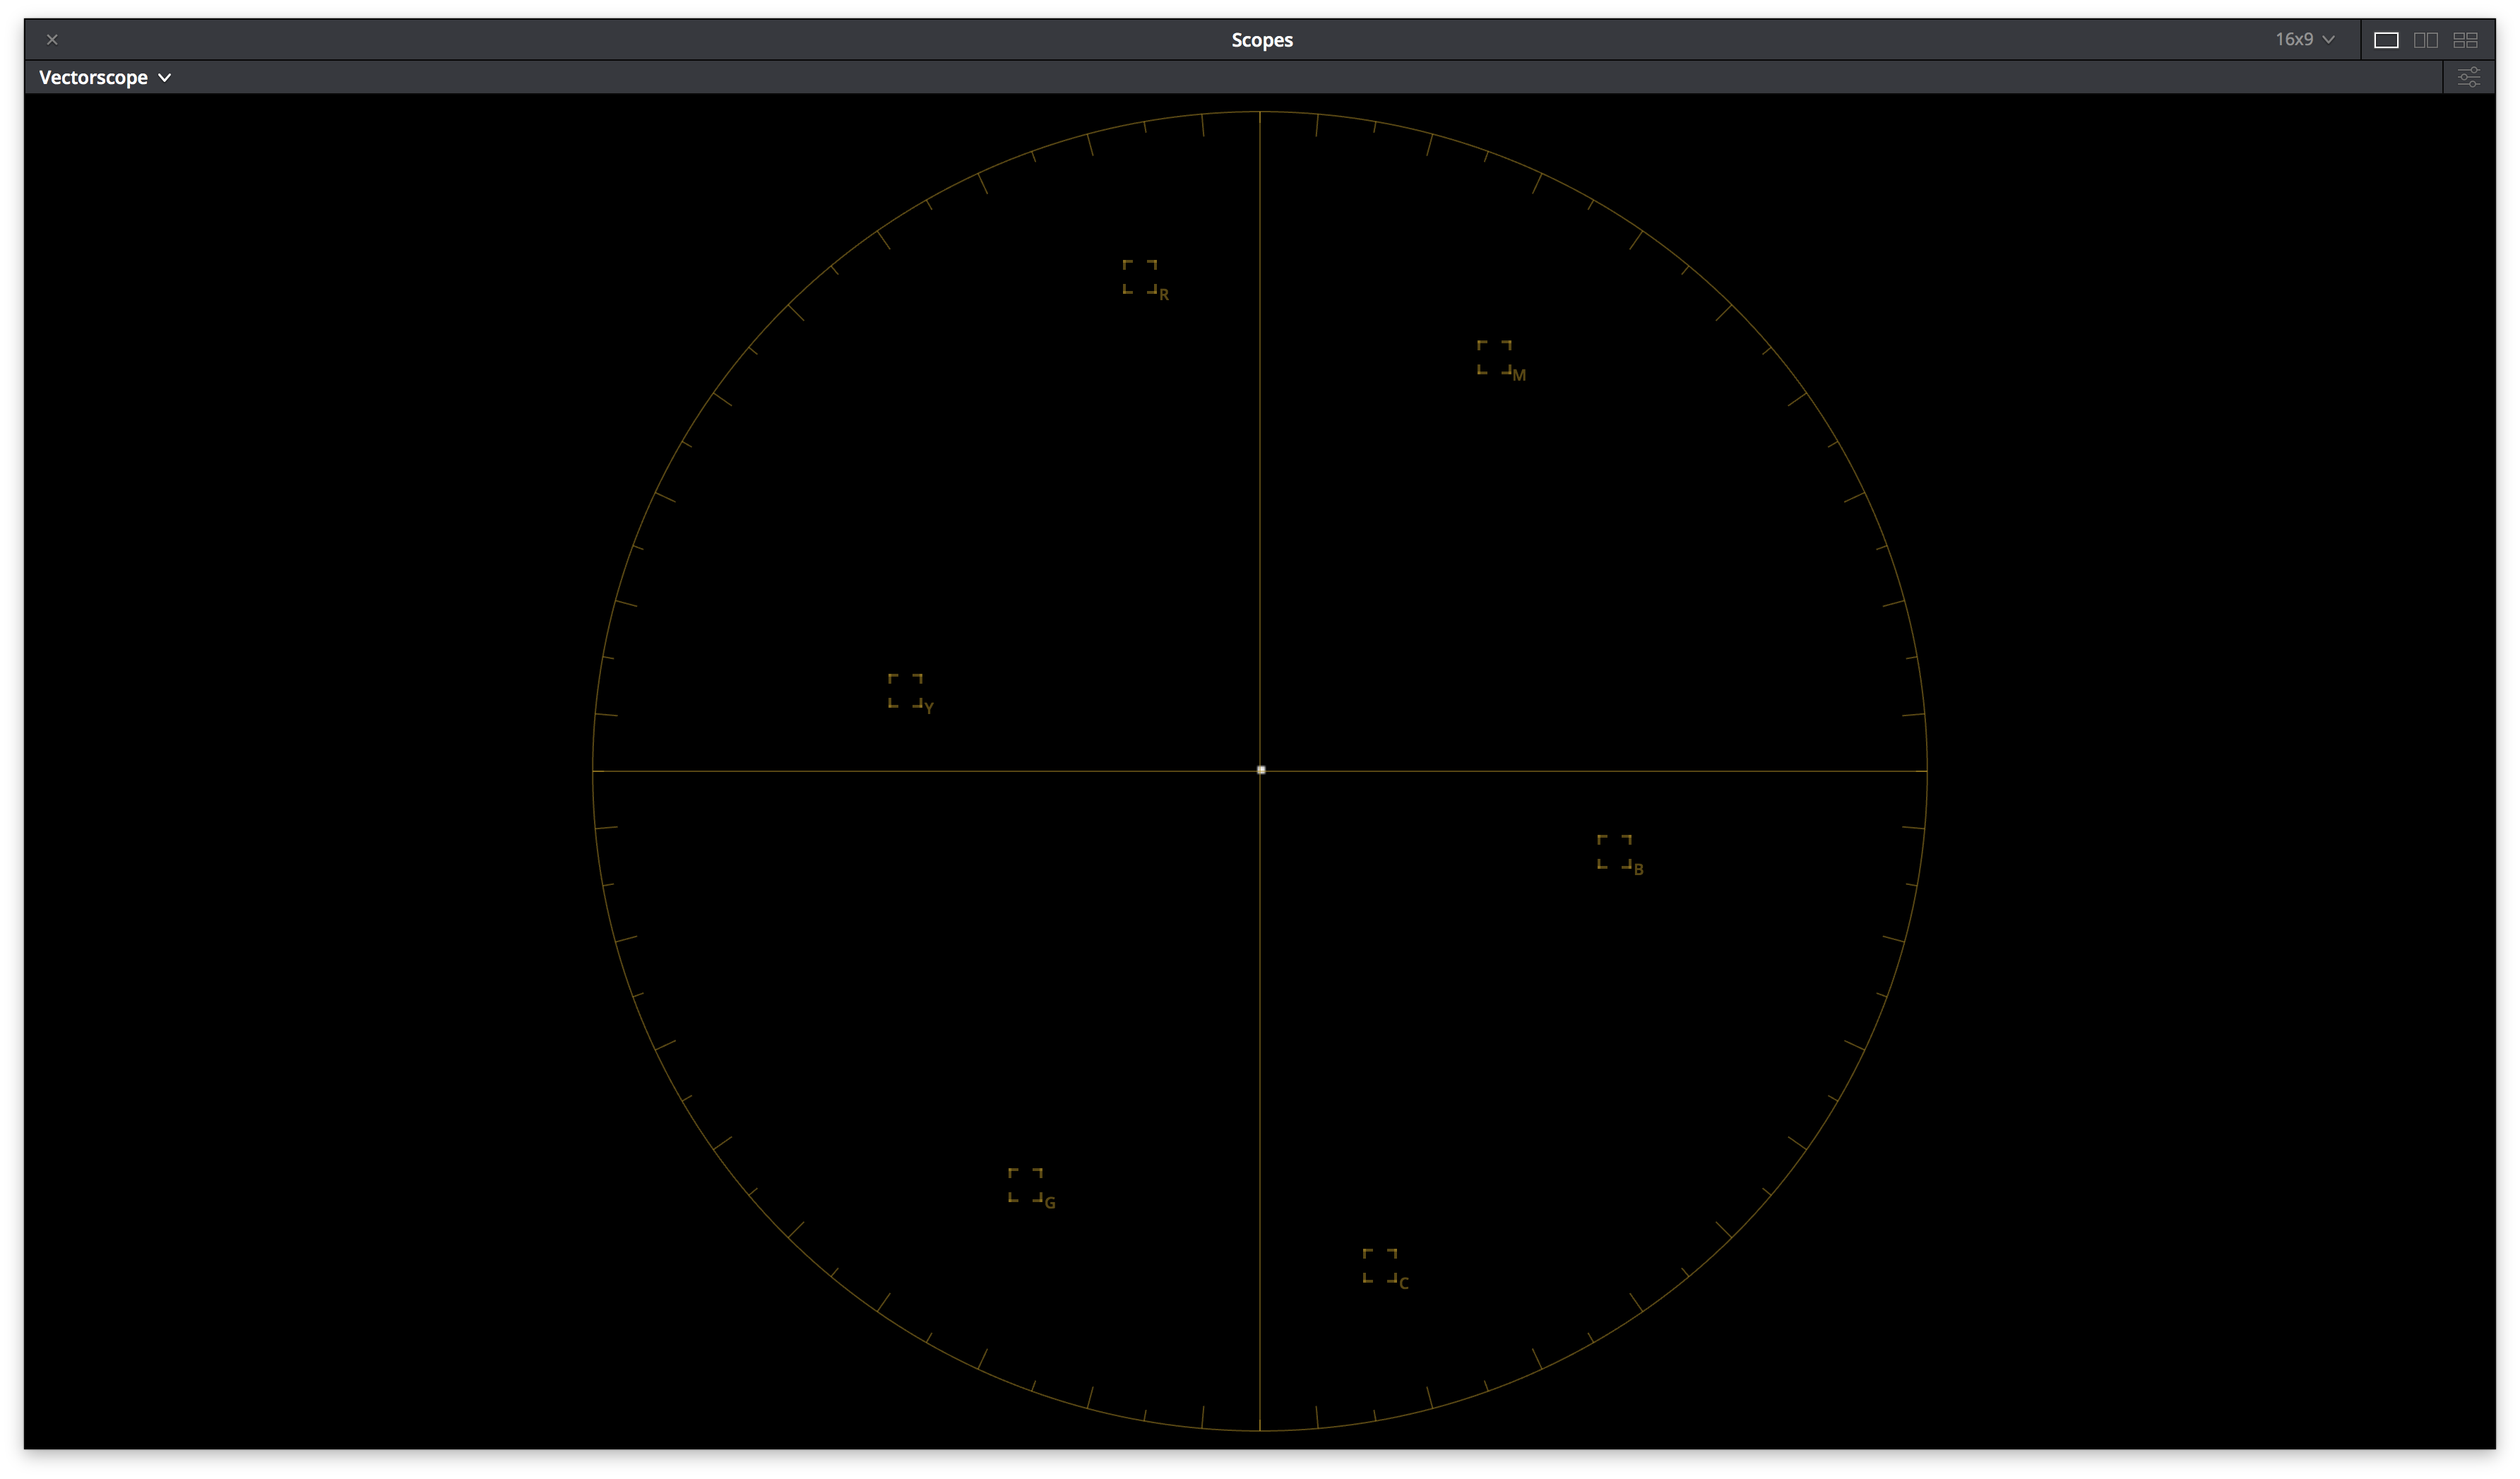
\includegraphics[width=\textwidth]{images/rec709/rec709_vectorscope}
            \caption[]%
            {{\small vectorscope}}    
            \label{fig:vect-rec709}
        \end{subfigure}
        \quad
        \begin{subfigure}[b]{0.475\textwidth}   
            \centering 
            
\includegraphics[width=\textwidth]{images/rec709/rec709_image}
            \caption[Projector code values as displayed on a D65 calibrated computer monitor]%
            {{\small Projector code values as displayed on a D65 calibrated computer monitor}}    
            \label{fig:cv-rec709}
        \end{subfigure}
        \caption[]
        {\small \texttt{\seqsplit{ODT.Academy.Rec709\_100nits\_dim.a1.0.3}} Scope Screenshots} 
        \label{fig:screenshots-rec709}
    \end{figure*}

\subsection{Test Values}
\label{subsec:testValues-rec709}

Table \ref{tab:testValues-rec709} contains test values can be used to confirm the proper monitor setup and ODT combination.  Each of the 9 ACES RGB input values should yield the RGB noted display RGB code values (normalized 0-1, full range) when processed through the \texttt{\seqsplit{ODT.Academy.Rec709\_100nits\_dim.a1.0.3}}. When driving a properly setup display with the noted display RGB code values, the light from the display should measure with the noted CIE xyY colorimetry.  

If the display RGB code values do not match those in the table when using the corresponding input ACES RGB code values, it is likely the wrong ODT is being used.  If the proper display RGB code values are being produced by the ODT, but he measured display colorimetry doesn't match the display xyY code values noted, it is likely the display setup is incorrect.

\begin{table}[ht!]
    \centering
    \begin{tabular}{|l|l|l|l|l|l|l|l|l|l|}
        \hline
        \multicolumn{1}{|c|}{\textbf{Patch}} & \multicolumn{3}{c|}{\textbf{ACES RGB}} & \multicolumn{3}{c|}{\textbf{Display RGB}} & \multicolumn{3}{c|}{\textbf{Display xyY}} \\ \hline
        \textbf{N1} & 1.8233 & 1.8233 & 1.8233 & 0.9000 & 0.9000 & 0.9000 & 0.3127 & 0.3290 & 77.6573 \\ \hline
        \textbf{N2} & 0.2753 & 0.2753 & 0.2753 & 0.5000 & 0.5000 & 0.5000 & 0.3127 & 0.3290 & 18.9465 \\ \hline
        \textbf{N3} & 0.0898 & 0.0898 & 0.0898 & 0.2500 & 0.2500 & 0.2500 & 0.3127 & 0.3290 & 3.5897  \\ \hline
        \textbf{R}  & 0.4689 & 0.1193 & 0.0417 & 0.8275 & 0.1525 & 0.1498 & 0.6155 & 0.3303 & 14.3569 \\ \hline
        \textbf{G}  & 0.3390 & 0.8068 & 0.0936 & 0.1500 & 0.8300 & 0.1500 & 0.3005 & 0.5889 & 46.0295 \\ \hline
        \textbf{B}  & 0.2162 & 0.1330 & 0.8711 & 0.1500 & 0.1500 & 0.8300 & 0.1566 & 0.0709 & 5.5935  \\ \hline
        \textbf{C}  & 0.5187 & 0.9138 & 1.0432 & 0.1500 & 0.8300 & 0.8300 & 0.2265 & 0.3287 & 50.5696 \\ \hline
        \textbf{M}  & 0.5800 & 0.2096 & 0.9086 & 0.8300 & 0.1500 & 0.8300 & 0.3207 & 0.1589 & 18.9661 \\ \hline
        \textbf{Y}  & 0.8237 & 0.9378 & 0.0855 & 0.8300 & 0.8300 & 0.1500 & 0.4164 & 0.5005 & 59.4021 \\ \hline
    \end{tabular}
    \caption[SDR Broadcast Television Mastering - Test Values]{ \texttt{ODT.Academy.Rec709\_100nits\_dim.a1.0.3} Test Values}
    \label{tab:testValues-rec709}
\end{table}

%%%% Application -- Broadcast Television On-Set Preview (Rec.709 SDR Reference Monitor) %%%% 
\clearpage
\section{Broadcast Television On-Set Preview (Rec.709 SDR Reference Monitor)}
\label{sec:ot-app-rec709onset}

\subsection{Summary}
\label{subsec:summary-rec709onset}

It has become common to preview of episodic television production on-set using a standard dynamic range (SDR) Rec.709  Reference Monitor. The display is typically configured such that equal red, green, and blue display code values will produce the chromaticity CIE x=0.3127 y=0.3290 (aka D65) on the screen. With the display configured in this manner, where the intention is to master content for broadcast, it is recommended that the ACES 1.0 ODT with the transformID \texttt{\seqsplit{ODT.Academy.Rec709\_100nits\_dim.a1.0.3}} be used.

\subsection{Display Setup}
\label{subsec:setup-rec709onset}

\begin{table}[ht!]
    \centering
        \begin{tabular}{|p{1.25in}|p{3in}|}
            \hline
            \textbf{Parameter} & \textbf{Setting} \\ \hline
            Max Luminance & 100 nits \\ \hline
            Display White Point & D65 \\ \hline
            Primaries & Rec.709  \\ \hline
            EOTF & BT.1886 \\ \hline
            Viewing Environment & dim \\ \hline
            Signal & RGB 4:4:4 (Full range or Legal Range) \\ \hline
            Bit Depth & 10 or 12-bit \\ \hline 
    \end{tabular}
    \caption[Broadcast Television On-Set Preview - Display Setup]{\small Rec.709 Display Setup} 
    \label{tab:setup-rec709onset}
\end{table}

\subsection{Best ODT for application} 
\label{subsec:bestODT-rec709onset}

\begin{table}[ht!]
    \centering
    \begin{tabular}{|p{1.6in}|p{3.1in}|}
        \hline
        \textbf{Simple Name} & \textbf{TransformID} \\ \hline
        ACES 1.0 Output - Rec.709 & \texttt{\seqsplit{ODT.Academy.Rec709\_100nits\_dim.a1.0.3}} \\ \hline
    \end{tabular}
    \caption[Broadcast Television On-Set Preview - Best ODT]{\small Broadcast Television Mastering ODT} 
    \label{tab:bestODT-rec709onset}
\end{table}

\subsection{Notes}
\label{subsec:notes-rec709onset}

\texttt{\seqsplit{ODT.Academy.Rec709\_100nits\_dim.a1.0.3}} is intended to be used with a broadcast display that configured such that equal red, green, and blue display code values produce a chromaticity CIE x=0.3127 y=0.3290 (aka D65) on the screen and the content is intended to be viewed in a typical home viewing environment. The output transform is configured such that neutral ACES source file values (ACES R=G=B) will produce equal
projector code values. In this application, the image resulting on the display will mimick the content as it will appear in broadcast television mastering.  Care should be taken to configure choose the proper output range as the ODT supports both full and legal range.

It's important to note that the image on display screen should be similar in color balance to content produced with other video workflows. The color corrector scopes should reflect this white balance similarity by producing equal red, green and blue display code values for neutral ACES source file values. The scopes may however appear different in range to some video workflows.  In ACES based workflows dynamic range of the source content is maintained by manipulating the content prior to the output transforms.  The shape of the output transform tone scale may be reflected in the display code values being monitored on the color corrector scopes.  This is common with other video workflows where a look-up table (LUT) is used.

    \begin{figure*}[ht!]
        \centering
        \begin{subfigure}[b]{0.475\textwidth}
            \centering
            
\includegraphics[width=\textwidth]{images/aces}
            \caption[Source ACES Image]%
            {{\small ACES Image}}    
            \label{fig:acesSource-rec709onset}
        \end{subfigure}
        \hfill
        \begin{subfigure}[b]{0.475\textwidth}  
            \centering 
            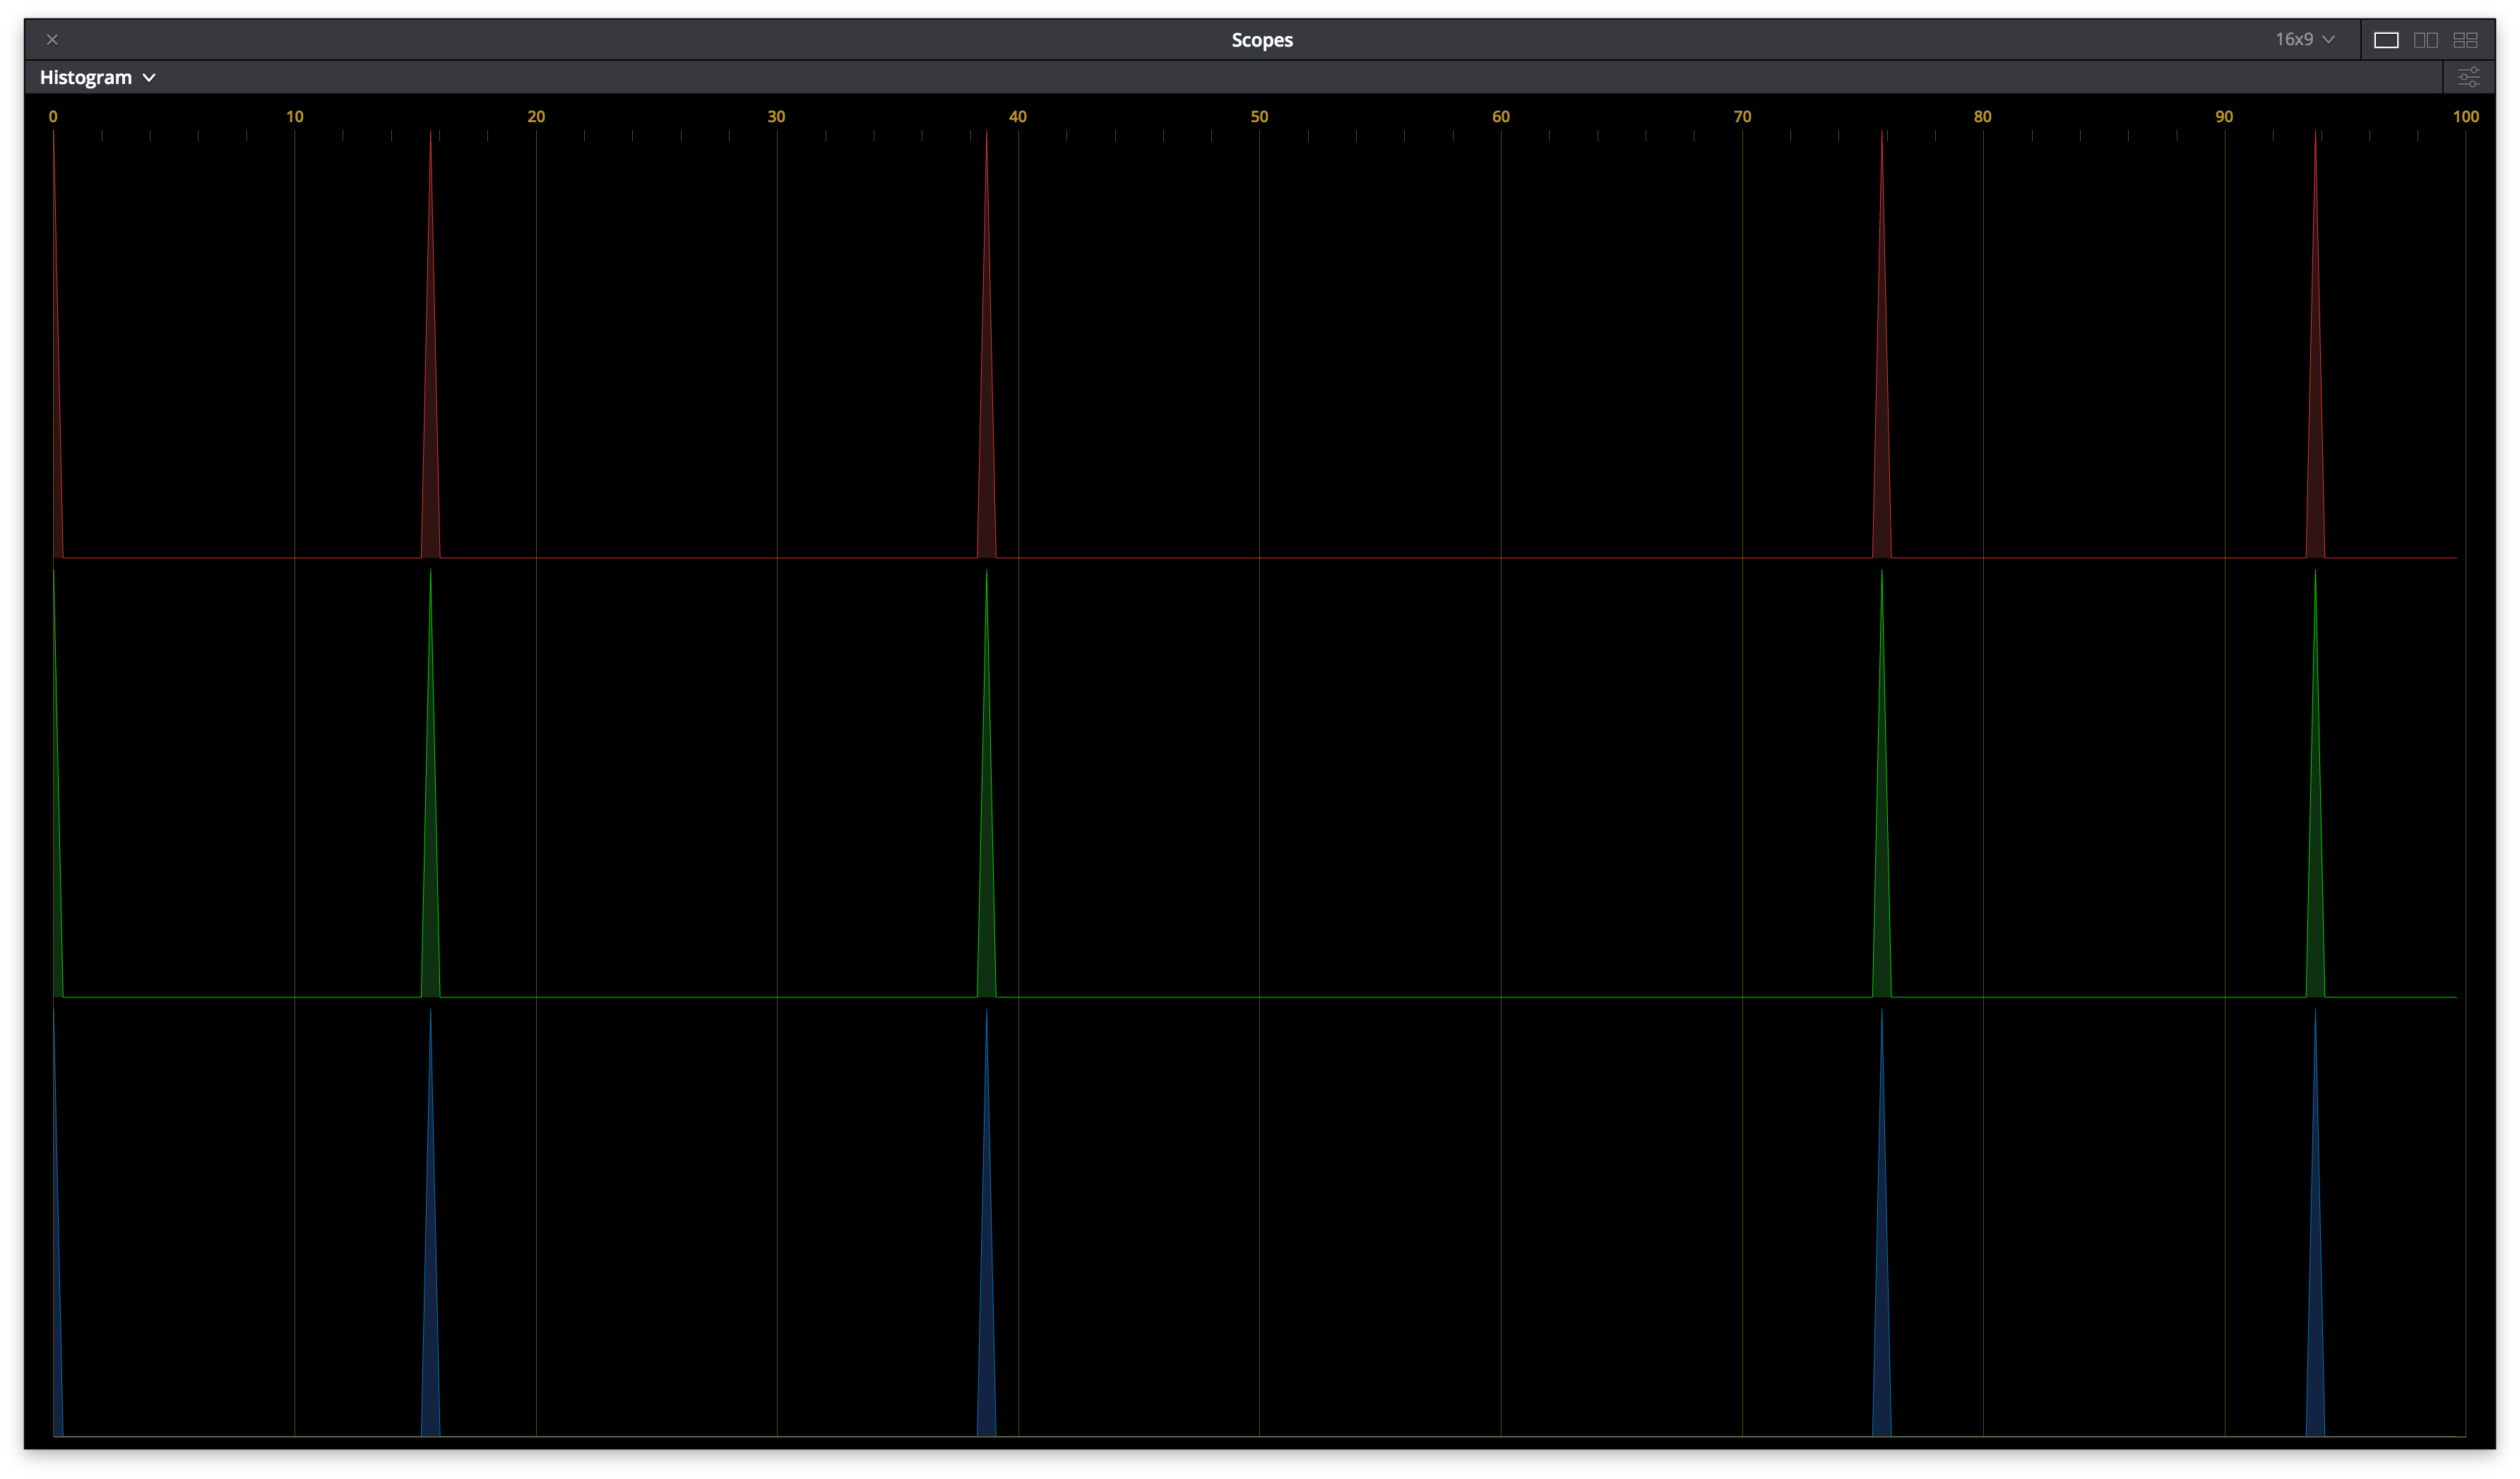
\includegraphics[width=\textwidth]{images/rec709/rec709_histogram}
            \caption[Histogram]%
            {{\small Histogram}}    
            \label{fig:hist-rec709onset}
        \end{subfigure}
        \vskip\baselineskip
        \begin{subfigure}[b]{0.475\textwidth}   
            \centering 
            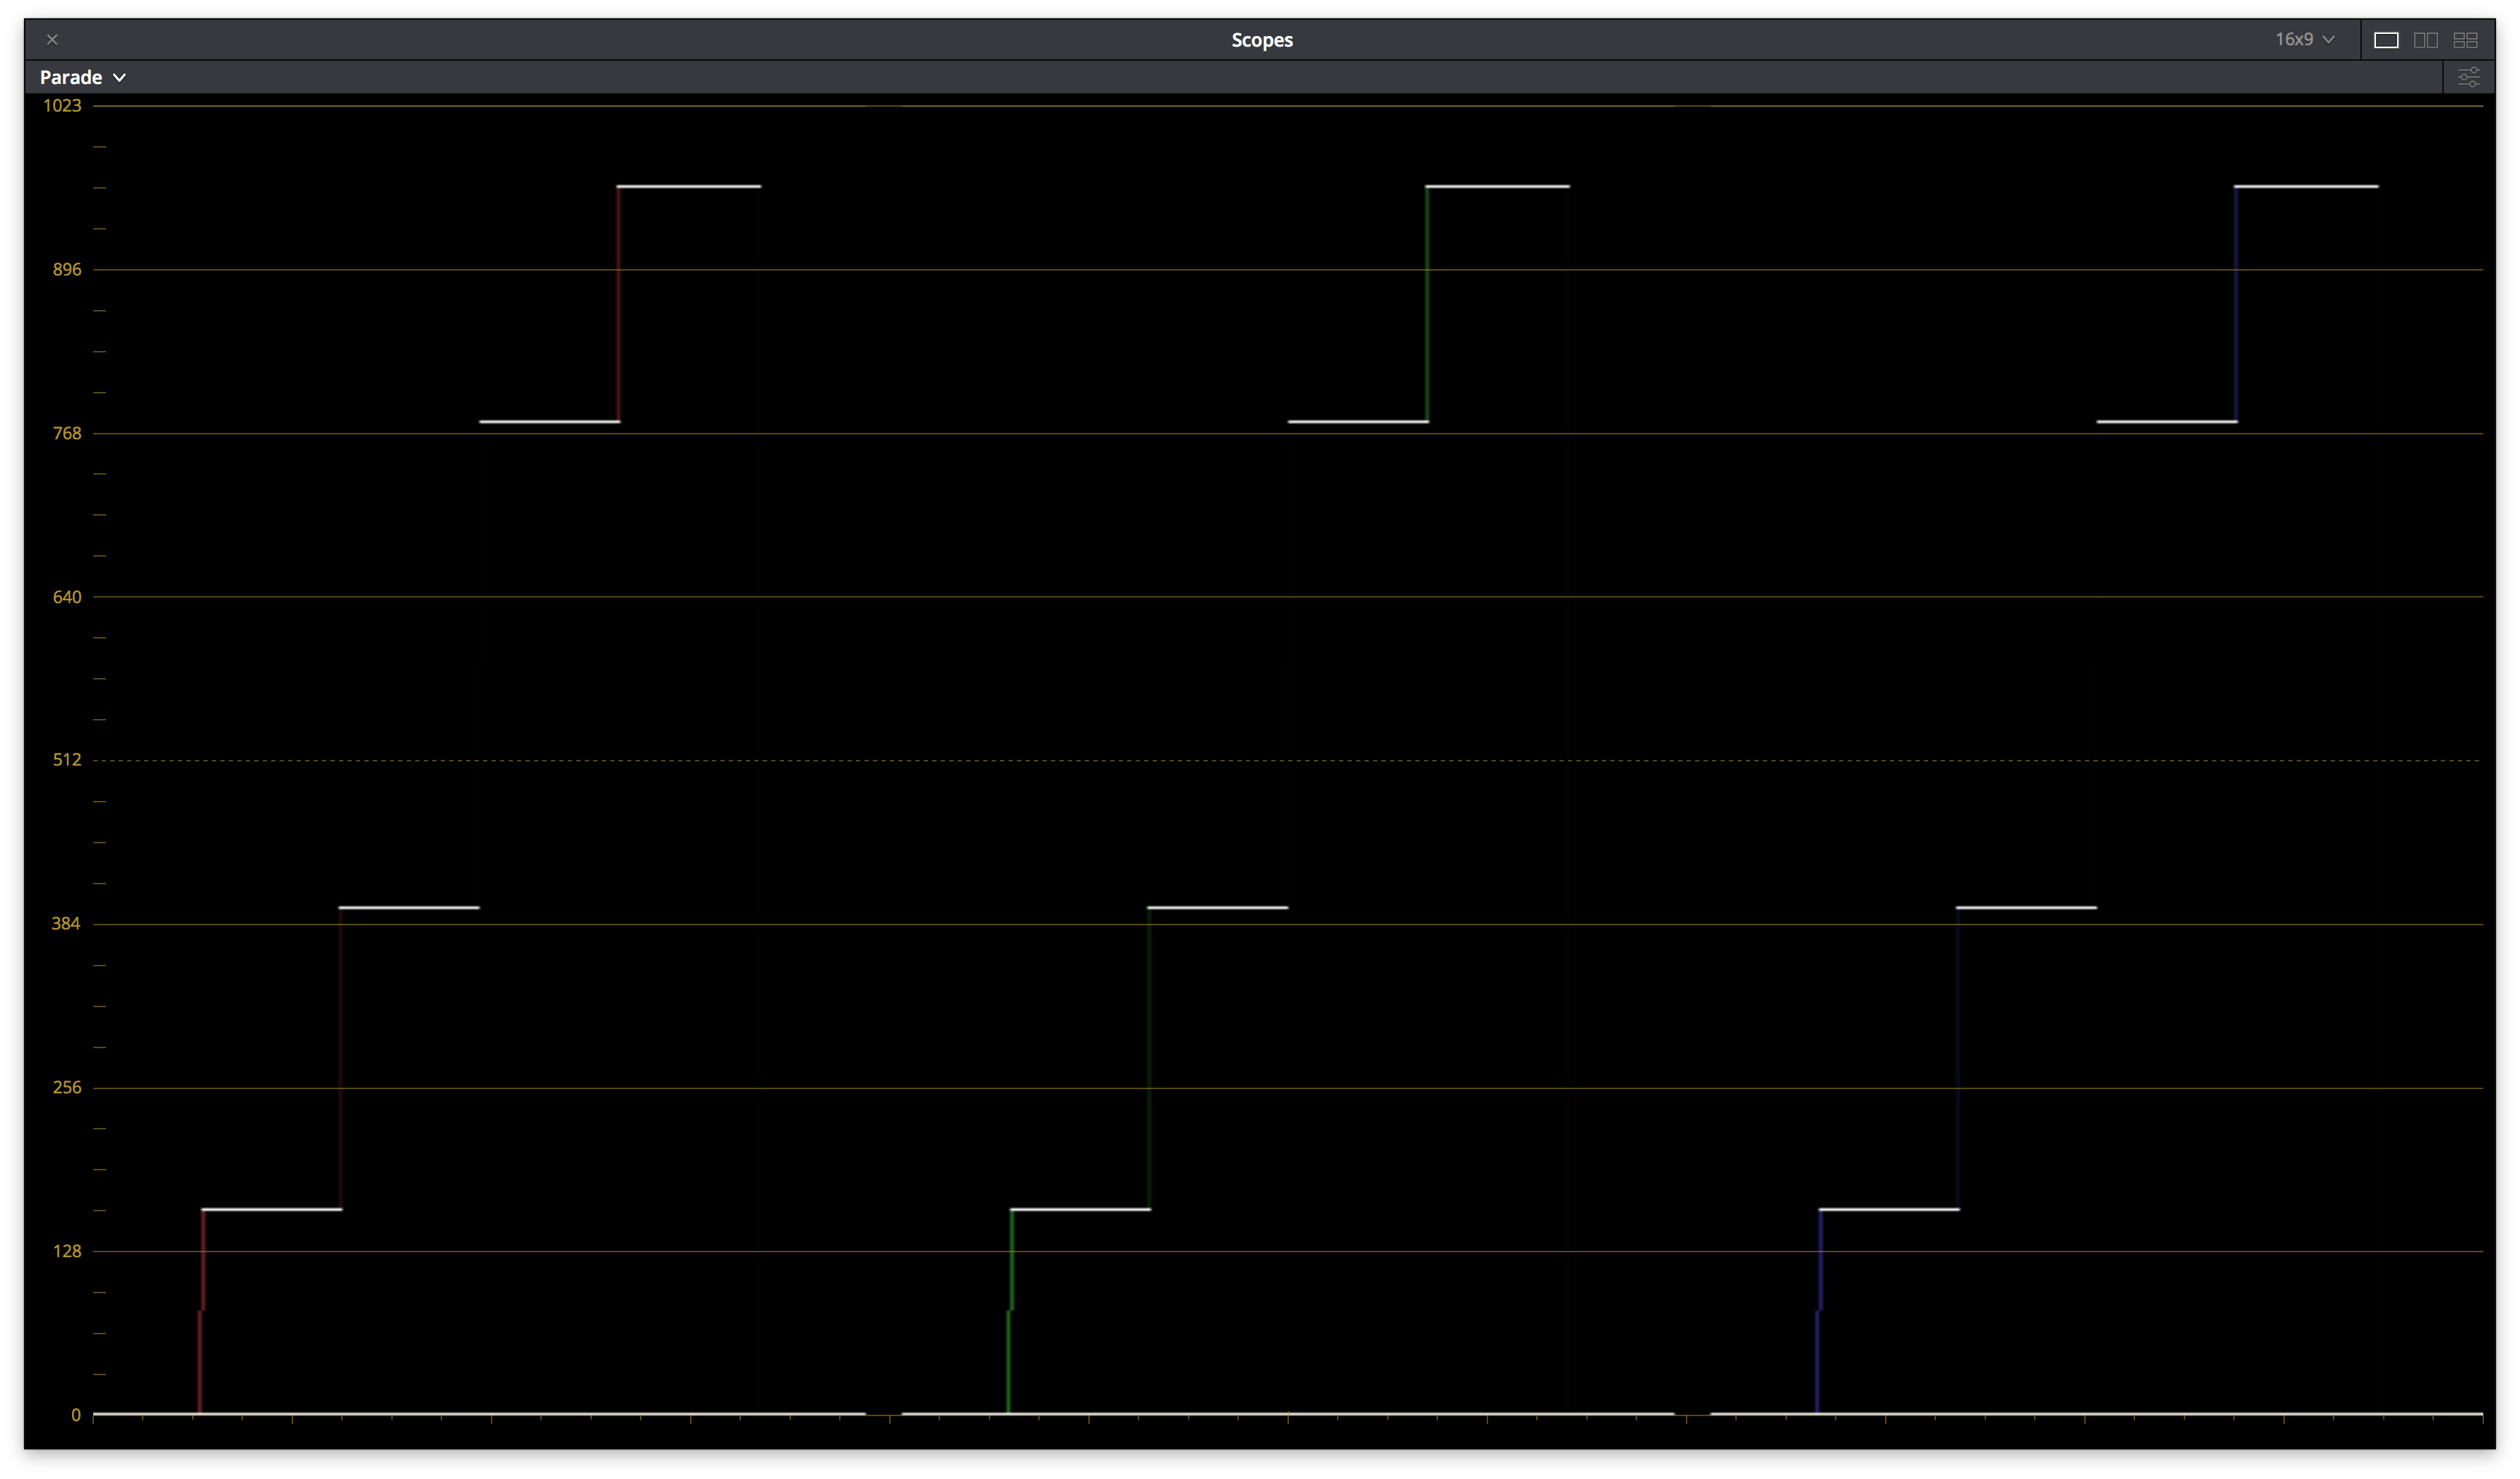
\includegraphics[width=\textwidth]{images/rec709/rec709_parade}
            \caption[Parade]%
            {{\small Parade}}    
            \label{fig:parade-rec709onset}
        \end{subfigure}
        \quad
        \begin{subfigure}[b]{0.475\textwidth}   
            \centering 
            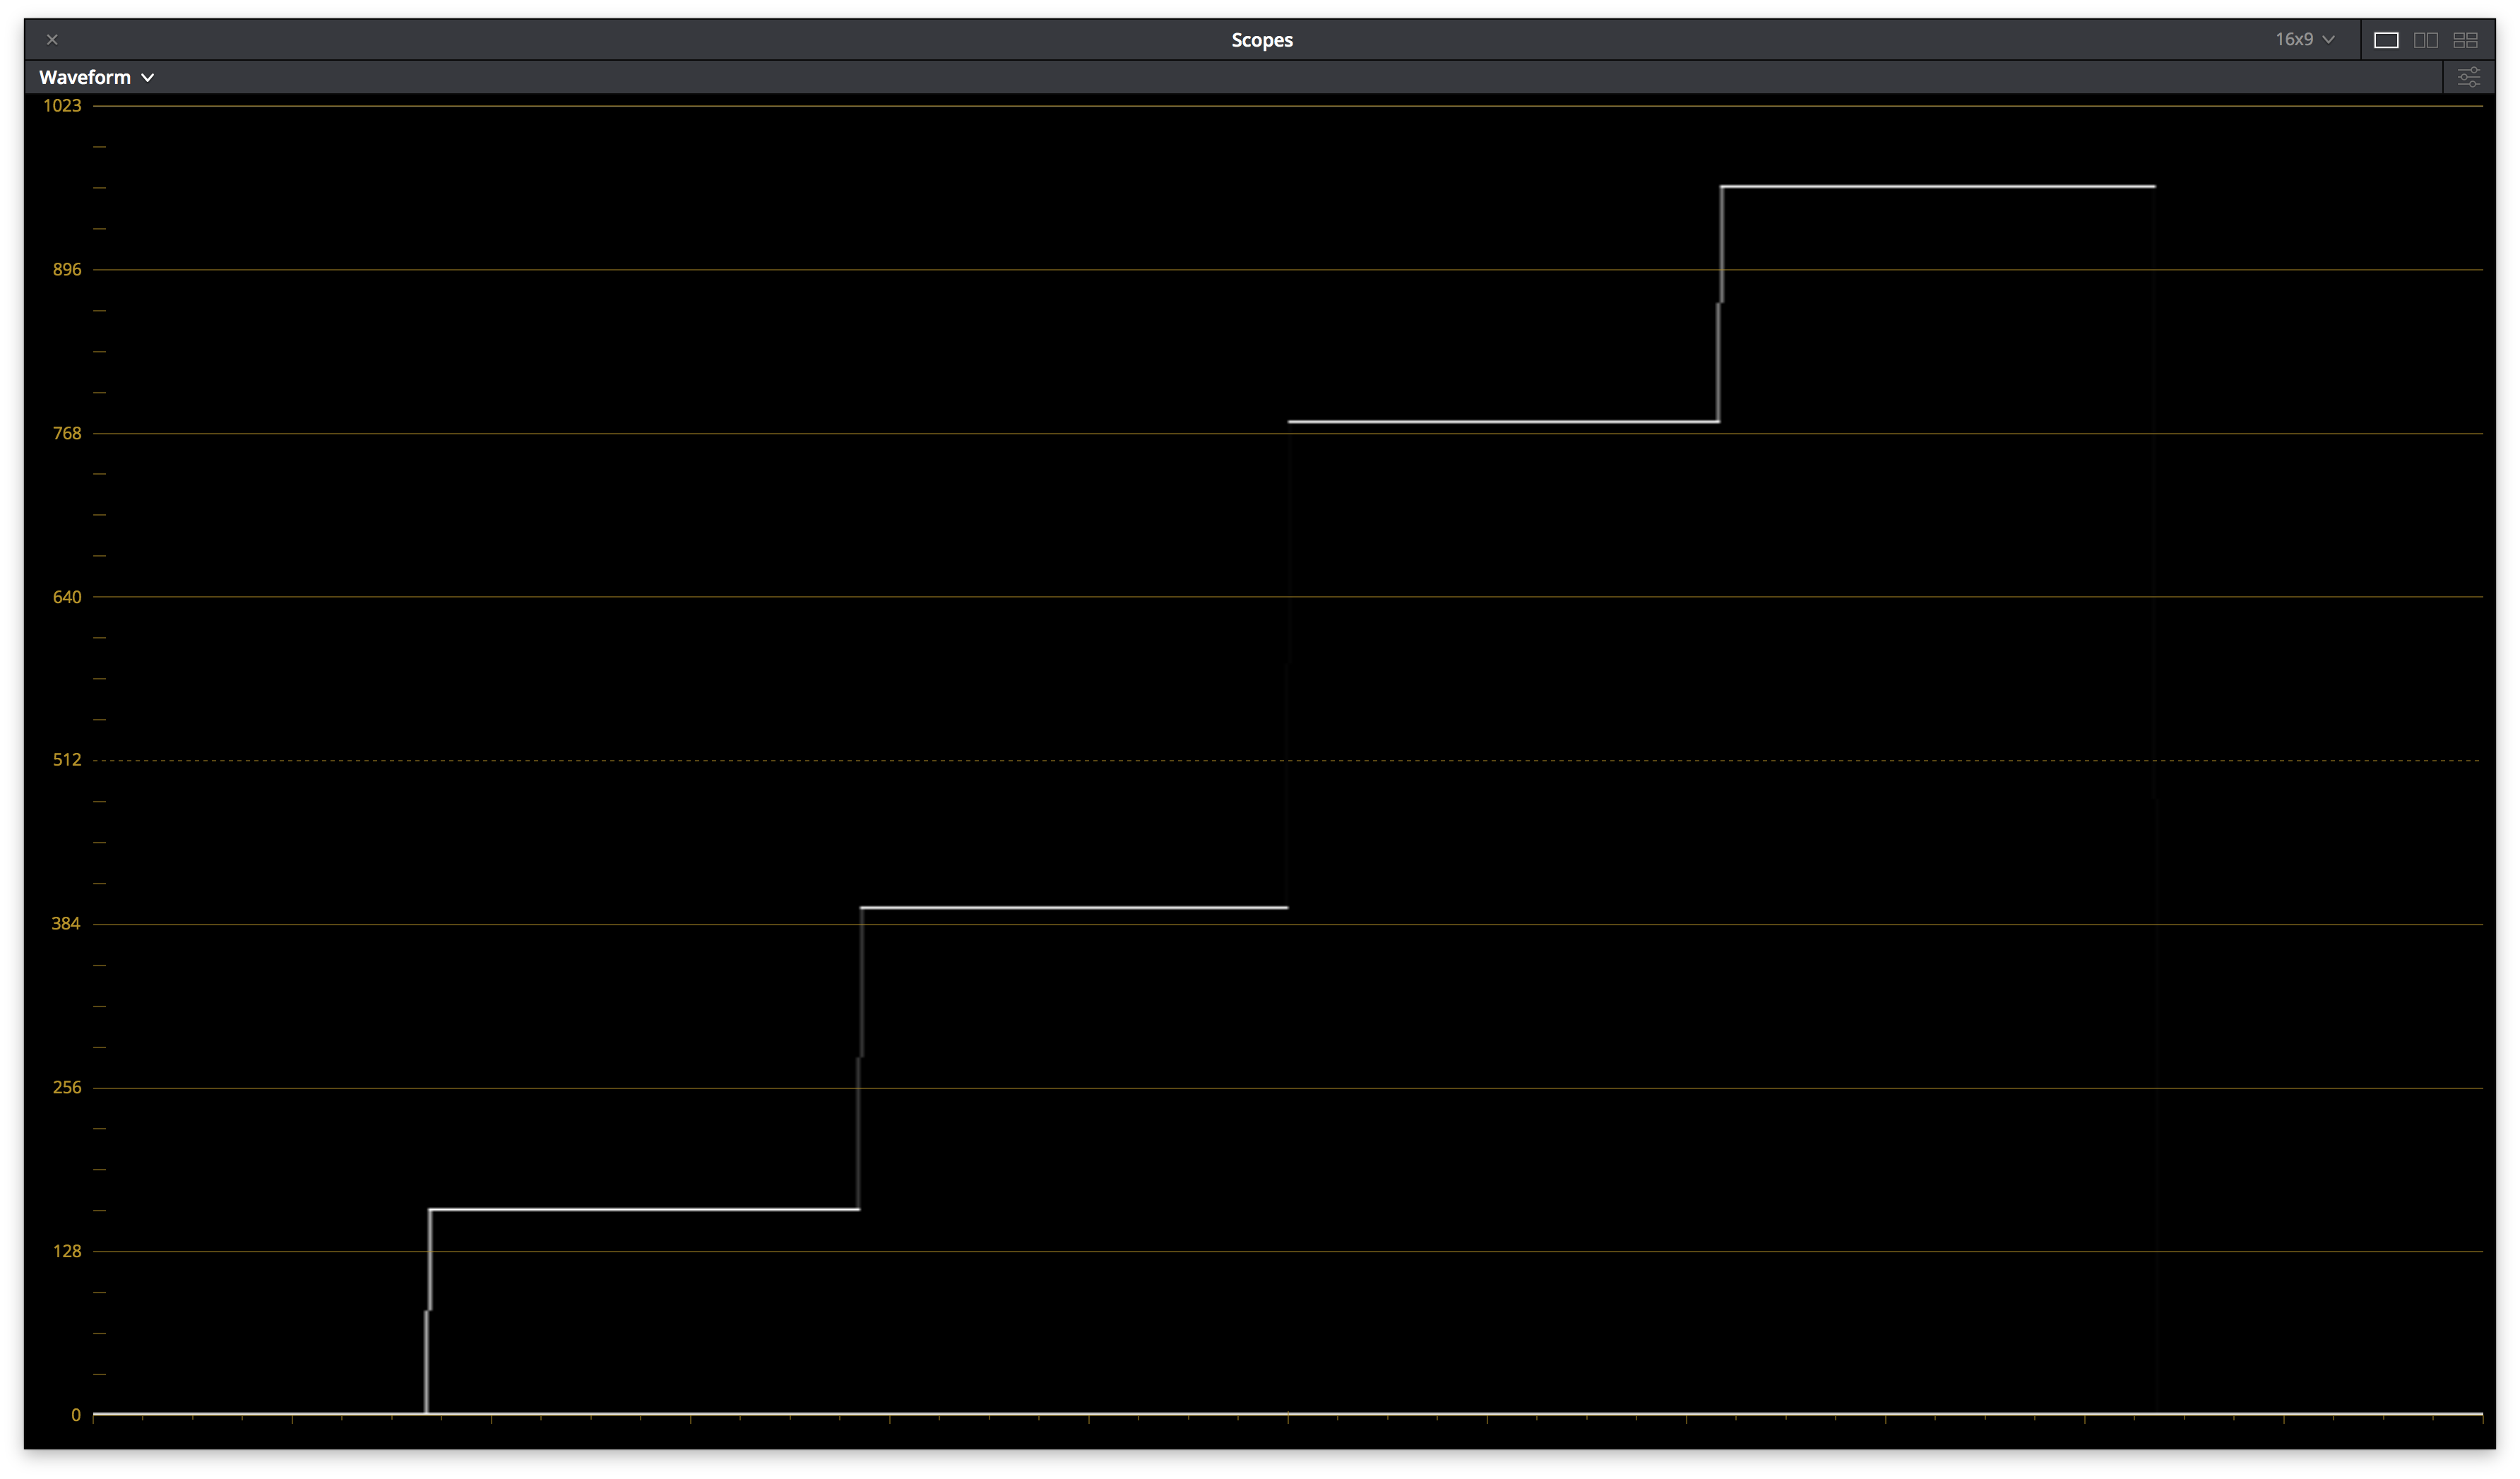
\includegraphics[width=\textwidth]{images/rec709/rec709_waveform}
            \caption[]%
            {{\small Waveform}}    
            \label{fig:wf-rec709onset}
        \end{subfigure}
        \begin{subfigure}[b]{0.475\textwidth}   
            \centering 
            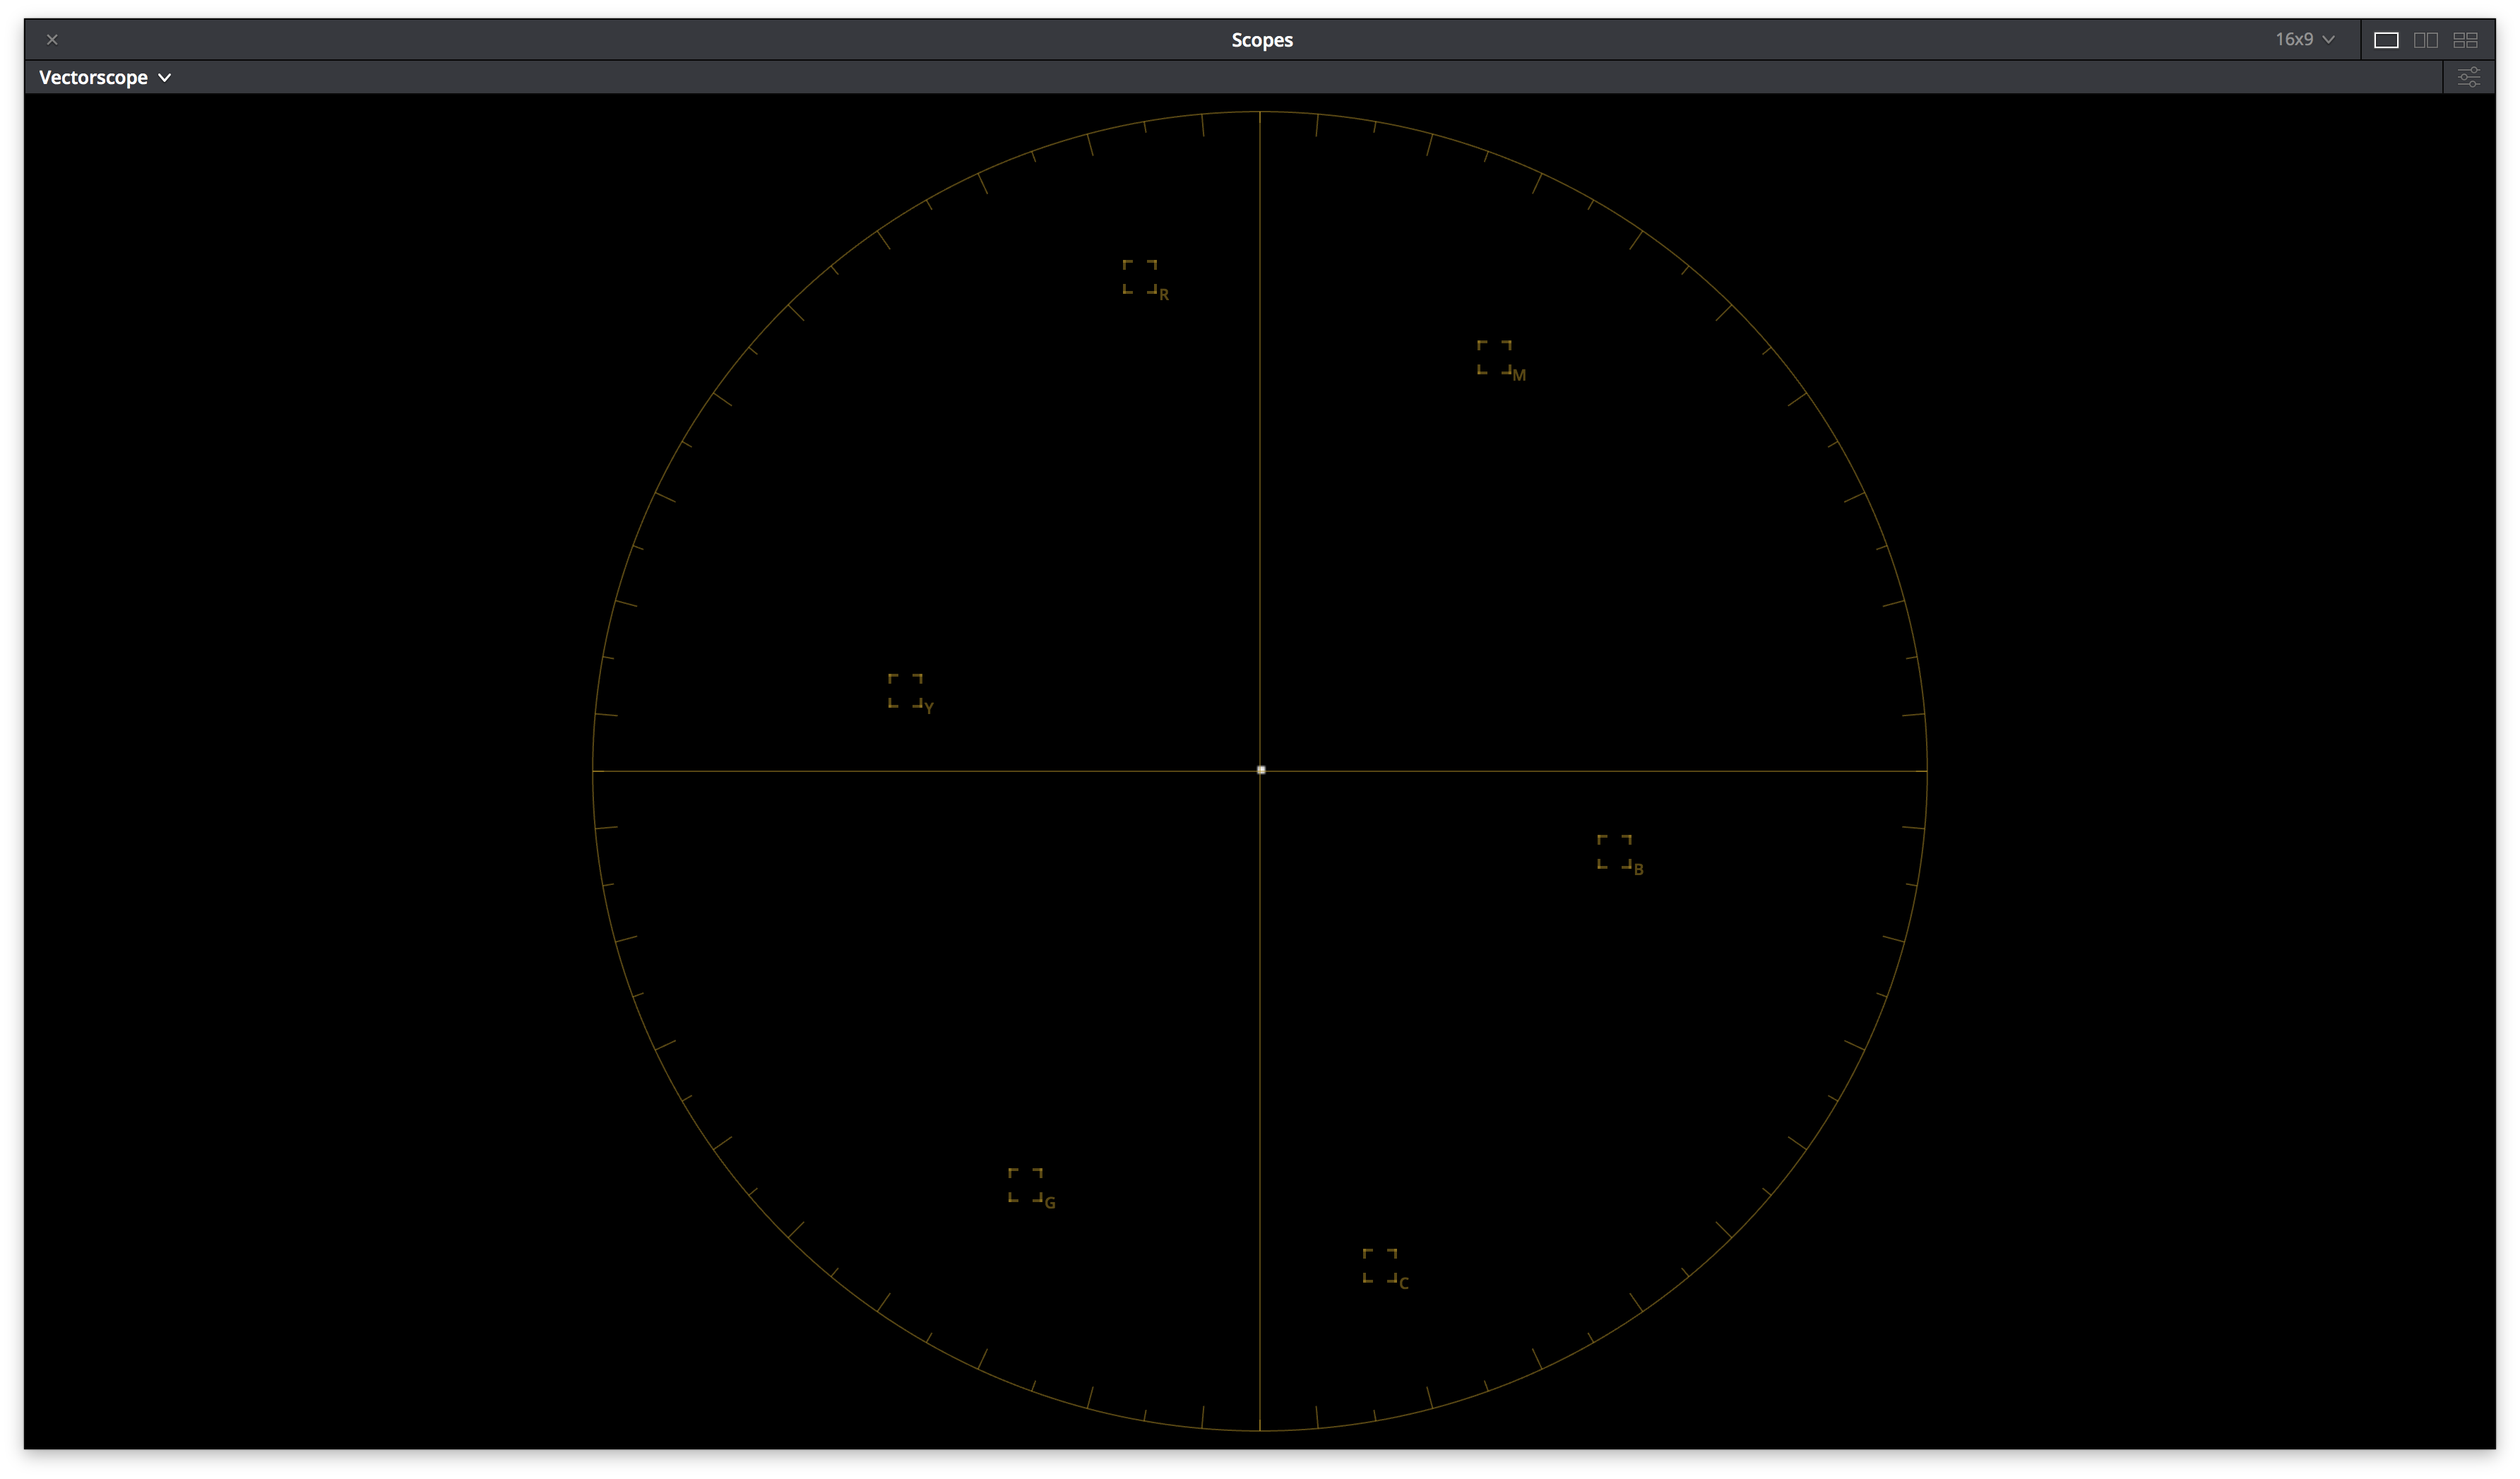
\includegraphics[width=\textwidth]{images/rec709/rec709_vectorscope}
            \caption[]%
            {{\small vectorscope}}    
            \label{fig:vect-rec709onset}
        \end{subfigure}
        \quad
        \begin{subfigure}[b]{0.475\textwidth}   
            \centering 
            
\includegraphics[width=\textwidth]{images/rec709/rec709_image}
            \caption[Projector code values as displayed on a D65 calibrated computer monitor]%
            {{\small Projector code values as displayed on a D65 calibrated computer monitor}}    
            \label{fig:cv-rec709onset}
        \end{subfigure}
        \caption[]
        {\small \texttt{\seqsplit{ODT.Academy.Rec709\_100nits\_dim.a1.0.3}} Scope Screenshots} 
        \label{fig:screenshots-rec709onset}
    \end{figure*}

\subsection{Test Values}
\label{subsec:testValues-rec709onset}

Table \ref{tab:testValues-rec709onset} contains test values can be used to confirm the proper monitor setup and ODT combination.  Each of the 9 ACES RGB input values should yield the RGB noted display RGB code values (normalized 0-1, full range) when processed through the \texttt{\seqsplit{ODT.Academy.Rec709\_100nits\_dim.a1.0.3}}. When driving a properly setup display with the noted display RGB code values, the light from the display should measure with the noted CIE xyY colorimetry.  

If the display RGB code values do not match those in the table when using the corresponding input ACES RGB code values, it is likely the wrong ODT is being used.  If the proper display RGB code values are being produced by the ODT, but he measured display colorimetry doesn't match the display xyY code values noted, it is likely the display setup is incorrect.

\begin{table}[ht!]
    \centering
    \begin{tabular}{|l|l|l|l|l|l|l|l|l|l|}
        \hline
        \multicolumn{1}{|c|}{\textbf{Patch}} & \multicolumn{3}{c|}{\textbf{ACES RGB}} & \multicolumn{3}{c|}{\textbf{Display RGB}} & \multicolumn{3}{c|}{\textbf{Display xyY}} \\ \hline
        \textbf{N1} & 1.8233 & 1.8233 & 1.8233 & 0.9000 & 0.9000 & 0.9000 & 0.3127 & 0.3290 & 77.6573 \\ \hline
        \textbf{N2} & 0.2753 & 0.2753 & 0.2753 & 0.5000 & 0.5000 & 0.5000 & 0.3127 & 0.3290 & 18.9465 \\ \hline
        \textbf{N3} & 0.0898 & 0.0898 & 0.0898 & 0.2500 & 0.2500 & 0.2500 & 0.3127 & 0.3290 & 3.5897  \\ \hline
        \textbf{R}  & 0.4689 & 0.1193 & 0.0417 & 0.8275 & 0.1525 & 0.1498 & 0.6155 & 0.3303 & 14.3569 \\ \hline
        \textbf{G}  & 0.3390 & 0.8068 & 0.0936 & 0.1500 & 0.8300 & 0.1500 & 0.3005 & 0.5889 & 46.0295 \\ \hline
        \textbf{B}  & 0.2162 & 0.1330 & 0.8711 & 0.1500 & 0.1500 & 0.8300 & 0.1566 & 0.0709 & 5.5935  \\ \hline
        \textbf{C}  & 0.5187 & 0.9138 & 1.0432 & 0.1500 & 0.8300 & 0.8300 & 0.2265 & 0.3287 & 50.5696 \\ \hline
        \textbf{M}  & 0.5800 & 0.2096 & 0.9086 & 0.8300 & 0.1500 & 0.8300 & 0.3207 & 0.1589 & 18.9661 \\ \hline
        \textbf{Y}  & 0.8237 & 0.9378 & 0.0855 & 0.8300 & 0.8300 & 0.1500 & 0.4164 & 0.5005 & 59.4021 \\ \hline
    \end{tabular}
    \caption[Broadcast Television On-Set Preview - Test Values]{ \texttt{ODT.Academy.Rec709\_100nits\_dim.a1.0.3} Test Values}
    \label{tab:testValues-rec709onset}
\end{table}

%%%% Application - Broadcast Television On-Set Preview (iPad) %%%% 
\clearpage
\section{Broadcast Television On-Set Preview (iPad)}
\label{sec:ot-app-iPad-d60}

\subsection{Summary}
\label{subsec:summary-iPad-d60}

Summarize the application in real world terms

\subsection{Best ODT for application}
\label{subsec:bestODT-iPad-d60}

\subsection{Notes}
\label{subsec:notes-iPad-d60}

\subsection{Test Values}
\label{subsec:testValues-iPad-d60}

%%%%%%%%%% application -- High Dynamic Range On-Set Preview %%%%%%%%%% 
\clearpage
\section{High Dynamic Range On-Set Preview (Rec.2020 HDR Reference Monitor)}
\label{sec:ot-app-rec2020hdr}

\subsection{Summary}
\label{subsec:summary-rec2020hdr}

Summarize the application in real world terms

\subsection{Best ODT for application}
\label{subsec:bestODT-rec2020hdr}

\subsection{Notes}
\label{subsec:notes-rec2020hdr}

\subsection{Test Values}
\label{subsec:testValues-rec2020hdr}

%%%%%%%%%% application -- Computer Visual Effects (VFX) Generation %%%%%%%%%% 
\clearpage
\section{Computer Visual Effects (VFX) Generation (Desktop Computer Monitor)}
\label{sec:ot-app-rgbMonitor}

\subsection{Summary}
\label{subsec:summary-rgbMonitor}

Summarize the application in real world terms

\subsection{Best ODT for application}
\label{subsec:bestODT-rgbMonitor}

\subsection{Notes}
\label{subsec:notes-rgbMonitor}

\subsection{Test Values}
\label{subsec:testValues-rgbMonitor}


%%%%%%%%%% application -- HDR10 Deliverable Generation %%%%%%%%%% 
\clearpage
\section{HDR10 Deliverable Generation (HDR 1000 nit Rec.2020 ST-2084)}
\label{sec:ot-app-hdr10}

\subsection{Summary}
\label{subsec:summary-hdr10}

Summarize the application in real world terms

\subsection{Best ODT for application}
\label{subsec:bestODT-hdr10}

\subsection{Notes}
\label{subsec:notes-hdr10}

\subsection{Test Values}
\label{subsec:testValues-hdr10}


%%%%%%%%%% application -- Dolby Vision Master %%%%%%%%%% 
\clearpage
\section{Dolby Vision Master (4000 nit Dolby Pulsar PQ Master)}
\label{sec:ot-app-doblyVision}

\subsection{Summary}
\label{subsec:summary-doblyVision}

Summarize the application in real world terms

\subsection{Best ODT for application}
\label{subsec:bestODT-doblyVision}

\subsection{Notes}
\label{subsec:notes-doblyVision}

\subsection{Test Values}
\label{subsec:testValues-dolbyVision}


% This file contains the content for a main section
\numberedformat
%% Modify below this line %%

\clearpage
\chapter{Recommended Workflows}
\label{ch:rec-workflows}
This section is intended to outline the recommended usage of ACES Output Transforms as they apply to common workflows applicable to feature motion picture and episodic television production.

%%%%%%%%%% Workflow %%%%%%%%%% 
\section{Feature Film Workflows}

\subsection{Production and Mastering -- SDR On-Set and Digital Intermediate}

\subsubsection{Summary}
It is common in the production of digital feature films to monitor the output of the camera on-set to check for framing, exposure, and often to create looks.  Looks are often created on-set or near-set using an on-set grading system with the result being a series of ASC-CDL values that are passed to digital intermediate (DI) mastering facility as a starting point for final grading.  In order to insure looks are set and communicated from on-set to the DI master facility as intended, it's important that the correct Output Transforms be used in each location.  The following is a recommendation for the usage of Output transforms for a common on-set to digital intermediate workflow.

\subsubsection{Workflow}
The complete workflow from camera to post is beyond the scope of this document, but Figure \ref{fig:workflow1} shows a typical workflow for the creation and communication of looks during feature film production.

\begin{figure*}[ht!]
\centering
    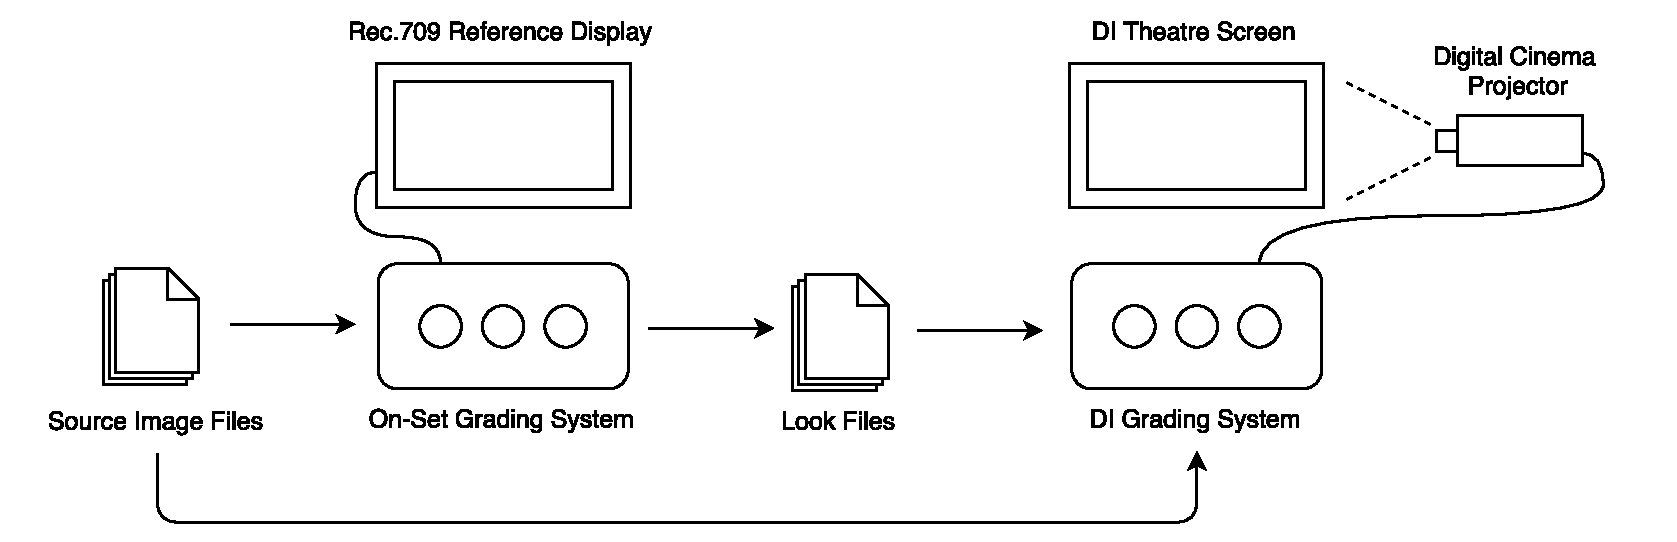
\includegraphics[width=4in]{images/workflows/workflow1.pdf}
    \caption{\small Feature Film On-Set to SDR DI Workflow}
    \label{fig:workflow1}
\end{figure*}

In this on-set to digital intermediate workflow a Rec.709 reference display is connected to the on-set grading system and a digital cinema projector is connected to the DI grading system.  In this workflow it is suggested that the on-set grading system be configured according to the Output Transform Application specified in Section \ref{sec:ot-app-rec709d60sim}.  The DI grading system should be configured according to the Output Transform Application specified in Section \ref{sec:ot-app-p3d60}, or alternatively Section \ref{sec:ot-app-p3dci}.  The recommendations are summarized in Table \ref{tab:sum-ff-os-workflow}.

\begin{table}[ht!]
\centering
\begin{tabular}{|p{0.5in}|p{1.2in}|p{3.75in}|}
\hline
\textbf{System}   & \textbf{Display}            & \textbf{Suggested ODT}                                                  \\ \hline
On-set \newline Grading & Rec.709 Reference Monitor   & \texttt{\seqsplit{ODT.Academy.Rec709\_D60sim\_100nits\_dim.a1.0.3}} \\ \hline
DI \newline Grading & P3 Digital Cinema Projector & \texttt{\seqsplit{ODT.Academy.P3D60\_48nits.a1.0.3}} \newline or \newline \texttt{\seqsplit{ODT.Academy.P3DCI\_48nits.a1.0.3}}           \\ \hline
\end{tabular}
\caption[Workflows - Feature Film (Onset-DI) - Suggested ODTs]{Summary of suggested ODTs}
\label{tab:sum-ff-os-workflow}
\end{table}

\subsubsection{Discussion}
In the On-Set to Digital Intermediate workflow, using the suggested ODT will provide a white point match between the two environments.  The displays will not match to the degree there are colors in the content that would take advantage of the P3 color space in DI since those colors could not be reproduced on-set with the Rec.709 monitor.  It's important to recognize that the colorimetry will not measure as matching due the the surround environment differences associated with the DI grading and On-set ODTs.  The On-set ODT is designed for a dim surround environment where the DI grading ODT is designed for a dark surround environment.  If viewed in their correct respective environments using the suggested ODTs should provide a visual match since the ODTs compensate for perceptual differences imposed by the viewing environments.

\subsection{Production and Mastering -- HDR On-Set and Digital Intermediate}
\subsubsection{Summary}
\subsubsection{Workflow}
\subsubsection{Discussion}

\subsection{On-set and Dailies -- iPad Review}
\subsubsection{Summary}
\subsubsection{Workflow}
\subsubsection{Discussion}

\subsection{Visual Effects}
\subsubsection{Summary}
\subsubsection{Workflow}
\subsubsection{Discussion}


\section{Episodic Television Workflows}

\subsection{Production and Mastering -- SDR On-Set and Digital Intermediate}
\subsubsection{Summary}
\subsubsection{Workflow}
\subsubsection{Discussion}

\subsection{Production and Mastering -- HDR On-Set and Digital Intermediate}
\subsubsection{Summary}
\subsubsection{Workflow}
\subsubsection{Discussion}

\subsection{On-set and Dailies -- iPad Review}
\subsubsection{Summary}
\subsubsection{Workflow}
\subsubsection{Discussion}

\subsection{Visual Effects}
\subsubsection{Summary}
\subsubsection{Workflow}
\subsubsection{Discussion}








\end{document}